\documentclass[12pt]{article}

\usepackage{amssymb,amsmath,amsfonts,eurosym,geometry,ulem,graphicx,caption,color,setspace,sectsty,comment,footmisc,caption,natbib,pdflscape,subfigure,array,hyperref}
\usepackage{hyperref}
\hypersetup{colorlinks,
citecolor=blue,
linkcolor=magenta
}
\usepackage{multirow}
\usepackage{booktabs}
\usepackage{graphicx}
\usepackage{lscape}
\usepackage{setspace}
\usepackage{tabularx} 
\usepackage{rotating}
\usepackage{tablefootnote}
\usepackage{amssymb}
\usepackage{array}
\usepackage{ragged2e}
\usepackage{nicematrix}
\usepackage{enumitem}
\usepackage{array} 
\usepackage{graphicx}
\usepackage{booktabs}
\usepackage{enumitem}
\usepackage{wasysym}
\usepackage{framed}
\usepackage{pgfgantt}
\usepackage{subfloat}
\usepackage{multirow}
\usepackage{blindtext}
\usepackage{graphicx}
\usepackage{lscape}
\usepackage{colortbl}
\usepackage{caption}
\usepackage{palatino}
\usepackage{mathpazo}
\usepackage[flushleft]{threeparttable}
\usepackage[margin=15pt,font=small,labelfont={bf,sf}]{caption}
%\usepackage{sectsty}
%\allsectionsfont{\sffamily}
\usepackage[semibold]{sourcesanspro}
\usepackage{sectsty}
\allsectionsfont{\sffamily}
% Bibliography
%\usepackage[style=alphabetic,sorting=nyt,sortcites=true,maxbibnames=5,autopunct=true,babel=hyphen,hyperref=true,abbreviate=false,backref=true,backend=biber]{biblatex}


\normalem

\doublespacing
\newtheorem{theorem}{Theorem}
\newtheorem{corollary}[theorem]{Corollary}
\newtheorem{proposition}{Proposition}
\newenvironment{proof}[1][Proof]{\noindent\textbf{#1.} }{\ \rule{0.5em}{0.5em}}

\newtheorem{hyp}{Hypothesis}
\newtheorem{subhyp}{Hypothesis}[hyp]
\renewcommand{\thesubhyp}{\thehyp\alph{subhyp}}
%\renewcommand{\familydefault}{\sfdefault} 
%\usepackage{kpfonts}
%\usepackage[T1]{fontenc}


\geometry{left=1.0in,right=1.0in,top=1.0in,bottom=1.0in}
\bibliographystyle{apalike}%aaai-named

\singlespacing
\title{\textbf{Has financialization changed the impact\\ of macroeconomic announcements?}\thanks{The authors thank participants at a seminar in Humboldt University Berlin and at meetings of the Commodity \& Energy Markets Association (2021),  World Finance \& Banking Association (2021), Société canadienne de science  économique (2022), 4th Ethical Finance and Sustainability (EFS) conference (2022), and Multinational Finance Society (2022), as well as Alessandro Melone, Jocelyn Grira and Joseph Marks (discussants). For financial support, the authors thank the Social Sciences and Humanities Research Council and the Chaire Industrielle-Alliance Groupe financier. Any remaining errors are ours alone.}}
%J'arrive pas le centrer dans le titre
\author{Simon-Pierre Boucher\footnote{PhD student in finance, Université Laval, Quebec City QC Canada G1V 0A6, email:   \texttt{simon-pierre.boucher.1@ulaval.ca}}\and Marie-H{\'e}l{\`e}ne Gagnon\footnote{Professor of Finance and Research Fellow, CRREP, Université Laval, email: \texttt{marie-helene.gagnon@fsa.ulaval.ca}}\and Gabriel J. Power\footnote{IG Wealth Management Chairholder, Professor of Finance and Research Fellow, CRREP and CRIB, Université Laval, email:   \texttt{gabriel.power@fsa.ulaval.ca}}
}
%\author{ANONYMOUS VERSION}
\date{ \today \\ First version: June 2021}
\begin{document}
\begin{titlepage}
\maketitle



\singlespacing


\begin{abstract}
\noindent 
%Turmoil in commodity markets can threaten a sustainable energy future.
%The transition to a sustainable energy future requires considerable investments, which can be discouraged by heightened volatility in commodity markets.
 We investigate, using high-frequency data, how financialization has affected the impact of macroeconomic announcements on commodity futures returns and volatility. We find that greater financialization dampens the impact of macroeconomic release surprises on commodity markets, as measured by price drift and volatility changes. This finding is consistent with prior literature suggesting that financial participants improve liquidity and price discovery, while reducing volatility. Since traditional market participants prefer stability, our results suggest a beneficial impact of financialization. However, by disaggregating the results, we also find that the effects of greater participation by swap dealers and money managers differ.%, especially for pro-cyclical commodities such as crude oil and natural gas.

\vspace{0.2in}
\noindent\textbf{Keywords:} commodities, energy, futures,  spillover, financialization, high-frequency, sustainable, commercial, institutional, volatility, macro, announcements, surprise, events.\\


\bigskip
\end{abstract}
\setcounter{page}{0}
\thispagestyle{empty}
\end{titlepage}
\pagebreak \newpage




\doublespacing

\section{Introduction} \label{sec:introduction}


%The financialization of commodities appears to have affected in particular the energy sector \citep{Singleton2014}. This is not surprising, given the dependence of our societies on fossil fuels. However, with the growing need for a green energy transition, it is reasonable to believe that financialization will also affect the metals sector as these commodities are used in new technologies (such as electrical car batteries) to achieve this transition. 
 %%INTRO
%Despite all those concerns financialization could be helpful for the development of sustainable energy market.
%If financialization  decreasing volatility, in commo and energy markets, it could foster greater investment in green energy sustianble transition. In fact, real option theory suggests that volatility disoucrages investment. Real option value theory means that volatility discourages investment because of option value of waiting when volatility is higher. Kellogg reference.
%This implies that fostering commodity market stability should improve investment in green energy sustainable transition.
%As more stable commodity markets would plausibly lead to greater investment in greeen transitition energy, it is relevant to investgiate to whether occurred in recent times and its impact on the underlying price distribution as it  as more widrespread market could be a step towards more  Sustainable, affordable and accessible raw energy markets.
%%Carbon markets could help


Since the early 2000s, commodities have gained popularity among non-traditional market participants such as hedge funds and index traders, mainly for diversification or speculative purposes. Despite investment outflows in 2009 (the Great Recession) and 2014-2016 (a global commodity slump linked to oversupply and weak demand), commodities remain popular on Wall Street. Indeed, 2022 may be a year of record commodity trading profit for firms such as Macquarie Group, Goldman Sachs and JPMorgan Chase, with an estimated \$18 Bn in profit for the top 100 banks.\footnote{See for example the Wall Street Journal, September 9th 2022, ``Wall Street’s Commodity Traders on Track to Break Profit Records''.} What is often called the financialization of commodities consists of several important market and regulatory changes affecting how commodities (futures, options, swaps and physicals) are traded by institutional and other non-traditional investors. Such increases in speculation and long-only index positions in commodity markets have been pointed out by some industry participants as being responsible for, respectively, increases in volatility and correlation between different commodities.\footnote{Helpful surveys of this large literature include \citet{boyd2018update} and \citet{cheng2014financialization}.} In this paper, we investigate financialization in commodity markets through the lens of macroeconomic announcement releases.

The financialization of commodities coincides, however, with a commodity bull cycle \citep*{humphreys2010great} that some refer to as a ``supercycle''.\footnote{Commodity price supercycles are extended periods during which commodity prices are substantially above their long-term trend (or below trend, for a bear cycle). According to the Bank of Canada, the last super cycle started in 1996 with a peak around 2011. This supercycle has not officially ended, but the rapid increase in the price of most commodities following the COVID-19 pandemic could potentially bring this cycle to an end.} During commodity bull cycles, traditional market participants voice concerns that prices may be distorted away from their fundamental values or that volatility is excessive, increasing the cost of hedging. For instance, \citet{masters2009testimony} argued that institutional investors disrupted commodity markets in the mid-2000s with the use of investment strategies typically reserved for financial securities. This claim has been, however, challenged by empirical research \citep*{irwin2011index,irwin2012testing,irwin2012financialization}. 


Financialization could affect commodity futures markets through risk sharing and information discovery \citep*{cheng2014financialization}.  In particular, investors can either provide liquidity to meet the hedging needs of other traders or consume liquidity when they trade for their own needs \citep*{kang2020tale}, thereby influencing liquidity risk. Price discovery in commodity markets is affected by informational frictions in the global supply, demand and inventories of commodities. Indeed, futures markets inform spot or cash markets, which are more decentralized. As a result, financialization could alter how commodity markets incorporate new information.

Given the importance to the economy of commodities and the growing interest of various financial players in this market, it is essential to understand how the information available to investors is propagated in the futures market. To the point of this paper, we can assess the impact of financialization by measuring how information discovery has been affected by the arrival of new players in the commodities market.


%  How do we get there
It is challenging to determine what information investors possess and through which channels prices are discovered. This paper considers macroeconomic announcement releases as a source of economically relevant information. The advantage of using announcements as a proxy for available information is that we know the precise timing of when the information is disclosed to investors.
In this paper, we assess the extent to which financialization affects commodity futures markets through their price reactions to surprises in macroeconomic announcement releases. Indeed, government statistical agencies collect, aggregate and release information about various aspects of the macro-economy, resulting in a substantial media and analyst coverage. We use high frequency data over the period of April 2nd, 2007 to December 29th, 2020 and  an event-study methodology similar to \citet*{andersen2007real} and \citet*{kurov2019price}. Our main empirical analysis focuses on six major commodity futures, with additional commodity results in the online appendix. 

In doing so, we examine the resolution of uncertainty, market efficiency, and how macroeconomic announcements are anticipated. High-frequency data allows for a greater degree of accuracy in measuring the impact of permanent and transitory news shocks on price volatility and returns.  Furthermore, using intraday data allows us to bypass a traditional criticism of event-study methods, which is that at a daily frequency, the effect of an announcement could easily be attributable to another market events \citep*[see e.g., ][]{kothari2007econometrics}. 
%Our paper builds on the financial literature on  information transmission in markets. \citet{goldstein2019commodity} show how financial participants in commodity markets affect futures price informativeness, bias, and comovement. Their model predicts that financialization initially improves, but eventually worsens, price efficiency measured through volatility. This paper also relates to \citet{brunetti2016speculators}, who show evidence on the positions held by different types of speculators. They show that hedge funds aid commodity markets by providing additional liquidity, resulting in more efficient prices. In contrast, merchant positions are positively correlated with volatility in crude oil and natural gas markets. 

%CONCLUSION. 
%This paper and the recent body of research suggests that financialization may contribute to sustanability alongside other instruments such as green bonds and portfolio screens for sustainable invvestments.
%In the coming years, it will be essential to assess whether the gradual shift away from fossil fuels is lessening the impact of financialization on futures contracts, and the link with commodity spot prices \citep{Knuth2018}.

%%CONTRIBUTION
Our main contribution is to present new insights on financialization by bridging this line of research with the macro announcements literature. To better identify the impact of announcements, this literature has moved from daily to high-frequency data, examining bonds  \citep*{andersen2007real, hu2013noise, balduzzi2001economic,lee1995oil, hautsch2011impact, kurov2019price}, stocks \citep*{andersen2007real,bernile2016can,kurov2019price} and foreign exchange rates \citep*{lee1995oil,andersen2003micro}. The use of high frequency data, however, is not widespread in commodity futures research \citep*{couleau2020corn}. We argue that the use of a lower sampling frequency for futures price returns in this literature could explain why no clear answer has emerged concerning the impact on volatility \citep*{tang2012index,brunetti2016speculators,irwin2012testing,stoll2010commodity,alquist2013role}. Since most of these studies use daily or monthly data, the resulting sample size is small, which reduces the power of statistical tests \citep*{irwin2009devil}.  



Our paper also builds on the financial literature on information transmission in markets. \citet*{goldstein2022commodity} develop theory to show how financial participants in commodity markets affect futures price informativeness, bias, and comovement. Their model predicts that financialization (defined as the increase in the number of financial speculators compared to financial hedgers in the commodity futures market) initially improves, but eventually worsens, price efficiency as measured through volatility. In addition, our analysis builds on a line of research on the effect of institutional investors. For instance,  \citet*{brunetti2016speculators} find that hedge funds add  liquidity to commodity markets, which results in more efficient prices. In contrast, merchant positions are positively correlated with volatility in crude oil and natural gas markets. 
%…. Il faudrait dire ce qu’ils entendent ici
%Thus, to better measure the impact of financialization, we look at information diffusion in the setting of high-frequency macro announcement releases. With these data, we can measure separately permanent and transitory, news-related shocks on volatility and price returns.
%Using high-frequency data further allows us to bypass a traditional criticism of event-study methods, namely that at a daily frequency, the effect of an announcement could easily be attributable to another market event \citep{kothari2007econometrics}. We focus on the US market due to the greater availability of high-frequency data on commodity futures as well as the wealth of distinct macro announcements.


Our second contribution is to provide disaggregated results by quantifying separately the involvement of fund managers and swap dealers, and to consider richer measures of financialization than those that are typically used. Prior research usually considers it sufficient to split the sample into pre- and post-financialization periods, with 2004 as the break point \citep*[see e.g., ][]{buyukcsahin2010matters, kilian2014role,brunetti2016speculators,irwin2012financialization,stoll2010commodity,alquist2013role}.\footnote{Although the Commodity Futures Trading Commission passed the Commodity Futures Modernization Act in 2000, the literature generally agrees that 2004 marks the beginning of financialization.} We argue that using this approach could neglect time-varying levels of non-traditional trader activity in the post-financialization period. Therefore, we use several measures of speculation based on the literature that are meant to proxy the time-varying level of financialization of each commodity. These measures are individually available for each commodity and therefore have the advantage of not treating the commodity market as a monolith when it comes to financialization. Indeed, the intensity of financialization measures varies not only over time but also between different commodities.  
%In addition, we provide deeper economic insights by separately quantifying speculation by fund managers and swap dealers. 
%Our second contribution is to consider richer measures of financialization than previously used. Research typically considers sufficient to split the sample into pre- and post-financialization periods, generally using 2004 as the break point \citep{buyukcsahin2010matters, kilian2014role,brunetti2016speculators,irwin2012financialization,stoll2010commodity,alquist2013role}.\footnote{Although the Commodity Futures Trading Commission passed the Commodity Futures Modernization Act in 2000, the literature generally agrees that 2004 marks the beginning of financialization.} While the timing is broadly accepted, using this approach neglects time-varying levels of non-traditional trader activity in the post-financialization period. In addition, we provide deeper economic insights by separately quantifying speculation by fund managers and swap dealers.
%%Most previous studies have assumed that financialization started in the early 2000s and that separating the sample into two groups (pre- and post-financialization) is sufficient to capture the impact of this phenomenon \citep{buyukcsahin2010matters, kilian2014role,brunetti2016speculators,irwin2012financialization,stoll2010commodity,alquist2013role}. 
%%it is well established that the period of financialization seems to have started in the early-to-mid 2000s
%
 %We summarize our findings as follows: First, we show that financialization contributes to information diffusion and price discovery. The impact of macro announcement surprises is typically dampened when  a given commodity is more affected by financialization. This result suggests that commodity markets are better informed--and macro news generate less of a shock--when commodities are financialized. This outcome should be beneficial to traditional commodity market participants.  This dampening effect  is stronger for pro-cyclical commodities such as crude oil or natural gas. In contrast, the evidence is weaker in the case of gold, a safe haven asset. %This result is particularly relevant for the energy commodity sector. 
%Second, we provide a disaggregated analysis by looking at money managers and swap dealers separately. We find that money managers contribute more to price discovery when there is a macro announcement while helping to reduce volatility. This result is consistent with the idea that money managers are more informed investors, given their role in the markets. Swap dealers also contribute to price discovery but are linked to an increase in volatility after macro announcements. Considering all categories of traders, greater levels of financialization overall seem to reduce  volatility in commodity markets. 
%Regarding policy implications, our results reject the \citet{masters2009testimony} hypothesis, according to which  financialization increases commodity price instability.  However, when we separate financial traders into two categories, our results allow us to reject  the \citet{masters2009testimony} hypothesis only for money managers. The evidence points a different way for swap dealers, suggesting they may contribute to commodity price instability. Lastly, the robustness tests we perform show that our main findings are robust to the use of alternative volatility measures and to differences in econometric specification.
%%and systemic risk%Thus, what we find is consistent with a considerable share of the literature.
%Finally, our paper also relates to energy transition shines a new light on financialization as it may prove helpful to develop sustainable energy markets. For instance, if financialization decreases volatility in commodity and energy markets, it could foster greater investment in energy transition. In fact, real option theory predicts that higher volatility discourages investment because the option value of waiting increases when volatility increases \citep{kellogg2014effect}.  Thus, stability in commodity markets may foster more investments in the energy transition. Moreover, analysts argue that the energy transition will initiate a new commodity supercycle.\footnote{See e.g. J.P. Morgan Asset Management,} These issues relate to the impacts of macroeconomics announcements as this transition may prove to alter the relationship between commodity markets and the real economy. 

% recap and summarize of important contributions
We summarize our findings as follows: First, financialization contributes to information diffusion and price discovery. The impact of a surprise following a macroeconomic announcement is generally dampened when a given commodity is more financialized. Therefore, commodity markets are better informed--and macro news generate less of a shock--when commodities are financialized. This outcome should be beneficial to traditional commodity market participants, who typically hold short position in the underlying asset.  This dampening effect is stronger for pro-cyclical commodities such as crude oil or natural gas. In contrast, the evidence is weaker in the case of gold, a safe haven asset that is less affected by macroeconomic announcements. 

Second, we find that money managers contribute more to price discovery and reduce volatility when there is a macro announcement. This result is consistent with the idea that money managers are more informed investors, given their role in the markets. Swap dealers also contribute to price discovery, but are linked to an increase in volatility after macro announcements. If we aggregate all categories of traders, greater levels of financialization overall seem to reduce volatility in commodity markets. Robustness checks show that our main findings remain true if we consider alternative volatility estimators, different econometric specifications, or if we change the financialization proxy. Thus, overall our results suggest that financialization is helpful to commodity markets, although this conclusion is contingent on the market composition of non-traditional traders. %Finally, our results show that financialization in the commodity market improves the overall functioning of this type of market.



%%%%%CE PARAGRAPHE EST MOINS PERTINENT POUR  J F Q A???. ON POURRA LE RAJOUTER POUR  E J.
Beyond implications for market participants and policymakers, the results may also be relevant to research on sustainable energy investments. The green energy transition shines a new light on the relevance of understanding the effects of financialization, as it could influence the development of sustainable energy markets. For instance, if financialization decreases volatility in commodity and energy markets, it could foster greater investment in energy transition. Indeed, real option theory predicts that higher volatility discourages investment as the option value of waiting (i.e., postponing investment) increases when volatility increases \citep*{kellogg2014effect}.  Thus, stability in commodity markets may foster more investments in the energy  transition. While most of the focus so far in this literature has been on energy firms, a large demand is also being created for the metals and minerals needed to build renewable energy infrastructures.\footnote{Moreover, analysts argue that the energy transition will initiate a new commodity supercycle.\footnote{See e.g., J.P. Morgan Asset Management, ``A new supercycle – the clean tech transition and implications for global commodities,'' February 24th, 2022. \url{https://am.jpmorgan.com/lu/en/asset-management/per/insights/market-insights/market-updates/on-the-minds-of-investors/clean-energy-investment/}}} \citet*{knuth2018breakthroughs} emphasizes that the gradual shift away from fossil fuels may lessen the impacts of financialization on futures contracts and their relationship with commodity spot prices. These issues point to the relevance of investigating whether financialization, through a broadening of the investor base, could be a step towards more sustainable, affordable and accessible raw energy markets.
% Taken together, these issues relate to the impacts of macroeconomics announcements as this transition may prove to alter the relationship between commodity markets and the real economy. 
%Carbon markets could help%As more stable commodity markets would plausibly lead to greater investment in  energy transition , i





%%%%%%%%%%%%%%%%%%%%%%%%%%%%%%%%%%%%%%%%%%%%%%%%%%%%%%%%%%%%%%%%%%%%%%%%%%%%%%%%%%%%%%%%%%%
%%%%%%%%%%%%%%%%%%%%%%%%%%%%%%%%%%%%%%%%%%%%%%%%%%%%%%%%%%%%%%%%%%%%%%%%%%%%%%%%%%%%%%%%%%%

%Include the tex file for Litterature review 

\section{Literature Review}
\subsection{Financialization of commodities}
The literature has not reached a consensus concerning the impact of financialization on commodity futures prices and volatility. Table 1 presents a summary of research findings on the influence of financialization and speculation on the volatility of commodity futures returns. On the theoretical side, \citet{basak2016model}’s model  yields four conclusions: (i) Prices of all commodity futures increase with financialization and this increase is more significant for futures belonging to the index than for non-indexed futures. (ii) The volatility of both index and non-index futures returns increases with financialization. (iii) Correlations between commodity futures returns, as well as equity-commodity correlations, increase with financialization. (iv) Only the prices of storable commodities are affected by financialization. 
%The literature has not reached a consensus concerning the impact of financialization on commodity futures prices and volatility. \citet{basak2016model} develop a theoretical model that yields four main findings suggesting a meaningful impact. (i) The prices of all commodity futures increase with financialization and this increase is more significant for futures belonging to the index than for non-indexed futures. (ii) The volatility of both index and non-index futures return increases with financialization. (iii) Correlations between commodity futures returns, as well as equity-commodity correlations, increase with financialization. (iv) Only prices of storable commodities are affected by financialization. Moreover, inventories and prices of storable commodities are higher in the presence of institutional investors than in the benchmark economy, and more so for commodities included in the index.

 The empirical evidence is mixed. On  the one hand, some of the literature provides support for the \citet{basak2016model} predictions. \citet{tang2012index} document increases in the correlations of crude oil and non-energy commodity returns, which they argue are due to the rapid growth of index investments in commodity markets. They argue that when a commodity is included in a benchmark index, its price is no longer determined solely by supply and demand. Rather, it is also determined by other commodities and assets included in the index. Moreover, \citet{singleton2014investor} shows that speculative activity by financial investors creates significant informational frictions, such that commodity prices can quickly move away from a value that is justified by fundamentals. He concludes that financialization can lead to considerable increases in volatility, as a result of information friction and prices deviating from values consistent with the economics of the commodity.
Moreover, \citet*{yang2005futures} show that when commodity futures trading volume increases, so does the volatility of commodity spot prices. 


On the other hand, a line of research finds no evidence that financialization is responsible for distorted prices or higher volatility. \citet*{stoll2010commodity} show that inflows and outflows from commodity index investments do not Granger-cause price or volatility changes. Using a no-arbitrage argument, \citet*{hamilton2014risk} show that the positions of commodity traders included in index funds cannot be used to achieve excess returns in futures markets. In addition, \citet*{kilian2014role} show that several speculative trades can occur in the oil market without seeing a significant change in inventory levels. This would seem to rule out speculation as being responsible for the boom and bust cycle in the oil market between 2003 and 2008. \citet*{bryant2006causality} reject the hypothesis that speculation and uninformed traders affect volatility. They show that the two theories that would predict this hypothesis, hedging pressure and normal backwardation, are empirically rejected and have no explanatory power. Lastly, \citet*{bohl2013does} show that financialization implies no change in conditional variance for daily returns on raw material futures.

\citet*{brunetti2014commodity} use an equilibrium model and data on trader positions in commodity futures markets to show that index traders provide insurance against price risk.   Closer to our paper,  \citet*{brunetti2016speculators}  analyze the impact of particular types of speculators in commodity markets from 2005 to 2009. They find that hedge funds allow for a faster and more efficient price discovery, resulting in a lower volatility. Furthermore, they find that the positions of swap dealers are not correlated with contemporaneous returns and volatility in commodity markets.  


 %Some studies differentiate the impact of different trader types, given their economic motivations. \citet{brunetti2014commodity}  use an equilibrium model and data on trader positions in commodity futures markets to show that index traders provide insurance against price risk.   Closer to this paper, \citet{brunetti2016speculators}  analyze the impact of certain types of speculators in commodity markets from 2005 to 2009. They find that hedge funds allow for faster and more efficient price discovery, resulting in a lower volatility. Furthermore, they find that the positions of swap dealers are not correlated with contemporaneous returns and volatility in the commodity markets.  \textcolor{red}{Table 1} presents a summary of the literature on the influence of financialization and speculation on the volatility of commodity futures returns.
  %%However, a consensus has not been reached in the literature.%   As for financialization linked to speculation,   Moreover,  

\subsection{Macroeconomic announcements}


\subsubsection{Macro announcements and financial markets}
A large empirical literature documents the impact of macroeconomic announcements on stocks \citep*{,scholtus2014speed} and bonds* \citep{fleming1997moves,fleming1999price}. In a seminal study, \citet*{balduzzi2001economic} investigate the effects of scheduled macroeconomic announcements on prices, trading volume, and bid-ask spreads. For each release, they measure the surprise in the announced quantity. Using intraday data from the interdealer government bond market, they find that 17 public news releases have a significant impact on the price of at least one of the following instruments: a three-month bill, a two-year note, a 10-year note, and a 30-year bond. Following a macro announcement, there is a persistent and significant increase in volatility and trade volume. The effects also vary by instrument maturity.

Other research has examined whether economic conditions can explain some of the more heterogeneous responses to announcements across business cycles. \citet*{andersen2003micro} find that the stock market reacts to news differently depending on the stage of the business cycle.  \citet*{boyd2005stock} also shows that the impact of unemployment-related announcements varies according to the economic environment.  Exploiting the fact that high-frequency traders receive the Michigan Consumer Sentiment Index two seconds before its official announcement, \citet*{hu2017early} find evidence of highly concentrated trading and rapid price discovery occurring within 200 milliseconds. Outside this narrow window, the typical investor trades at fully adjusted prices. 






%(see e.g. cite quelques papiers que j’ai enlevé)
\subsubsection{Macro announcements and commodity markets}

In the commodity literature on announcements, the focus so far has been on energy and in particular on OPEC meetings announcements.  \citet*{horan2004implied} find that volatility drifts upward as OPEC meetings draw nearer, then decreases after the first day of the meetings and continues to fall during a 5-day window. \citet*{wirl2004impact} assess the influence of OPEC on world oil markets by looking at fifty meetings from 1984 to 2001. They find little reaction in the markets to these meetings. \citet*{kilian2011energy} run daily frequency regressions of WTI crude oil and U.S. gasoline prices on 30 U.S. macroeconomic announcements from 1983 to 2008. They find no evidence of statistically significant responses for either oil or gasoline.  \citet*{gu2018drives} provide an explanation for the pre-announcement price drift in the natural gas market. They show that inventory surprises can be predicted using the difference between the forecast of the historically highly-accurate median analyst and the consensus forecast. The lack of conclusive results obtained by \citet*{wirl2004impact} and \citet*{kilian2011energy} may be due to the use of daily data for futures returns. We aim to overcome this problem by using high frequency returns. 


% to U.S. macroeconomic news at daily time horizons.
%vol decr by three percent and by five percent over a five-day window period


In an early study of announcement releases and commodities, \citet*{frankel1985commodity} find, using daily data, that a 1 percentage point positive shock in the money supply leads to a 0.7 percent decline in gold prices. \citet*{christie2000macroeconomics} analyzes the sensitivity of gold and silver futures prices over 15-minute intervals to 23 U.S. macroeconomic news announcements from 1992 to 1995. He finds that gold and silver price volatility is higher during days in which there are announcements. \citet*{cai2001moves} capture intraday patterns of 5-minute gold price variation using GARCH models around macro announcements. They find the intraday price effects of announcements to be fewer and less significant for gold than for bonds or currencies.  Likewise, \citet*{hess2008commodity} find that CRB and Goldman Sachs commodity indexes are less sensitive to the impact of 17 U.S. macro announcements than are bonds or stocks.  \citet*{hollstein2020volatility} look at how different economic variables affect the term structure of commodity futures volatility. They show that speculation and jobs-related macro variables have the largest impact on volatility. Lastly, \citet*{ye2021macroeconomic} quantify the impact of expectations about future economic conditions on commodity futures markets. They find that volatility in commodity futures seems to be more affected by macroeconomic forecasts than by current economic conditions. 

So far, the literature shows a clear impact of macroeconomic announcements on the price of stocks and bonds. However, there does not seem to be a consensus on whether announcements impact the price of commodity futures. Our research provides some insight into this issue by expanding the set of announcements beyond those which are normally used, such as OPEC. The other major element that contributed to the significant results and is also at the center of our contribution is the addition of variables quantifying the level of financialization for each of the individual commodities studied.




%Include the tex file for data
%%%%%%%%%%%%%%%%%%%%%%%%%%%%%%%%%%%%%%%%%%%%%
%%%%%%%%%%%%%%%%%%%%%%%%%%%%%%%%%%%%%%%%%%%%%
\section{Data sources, processing and variable definitions}
%We denote $R_t$ as the return over a period of 5 minutes starting exactly at time $t$. %contains, for all 5-minute intervals%of that 5-minute period  %%Subsequently, the return  by using $p_{t}^{Open}$ and $p_{t+\tau}^{Close}$
The publication (or release) of the realized value of a high frequency macroeconomic announcement affects markets \citep*{andersen1998deutsche}. To measure its impact, different methodologies have been considered.
 Here we describe our approach.  First,  to standardize and quantify the unexpected component (i.e., surprise) of a macroeconomic announcement release, we use the standardized surprise of an announcement rather than its realized value. For the calculation of the standardized surprise, we follow the approach detailed by \citet*{balduzzi2001economic}. Then, we use the standardized surprise in a regression model using high-frequency return data. Our regression model is based on frameworks described in \citet*{andersen2007real} for the specification and \citet*{kurov2019price} for modeling the error term.

Our data sources are as follows. For intraday data on commodity futures prices, we use Barchart's API.\footnote{ See the \url{https://www.barchart.com/futures} website.} The CFTC data on money manager and swap dealer positions are obtained from Quandl's API,\footnote{See the \url{https://data.nasdaq.com/data/CFTC-commodity-futures-trading-commission-reports} website.} and the macroannouncement announcement release data are collected from Bloomberg and Refinitiv.

\subsection{Data on macroeconomic announcements}
 
We collect information on 22 important and standard announcements \citep*[see e.g.,][]{andersen1998deutsche,kurov2019price}. The announcements can be broken down into ten categories: Income, Employment, Industrial Activity, Investment, Consumption, Housing Sector, Government, Net Exports, Inflation and Forward-looking. The majority of the announcements are released on a monthly basis. However, there are some exceptions, for which the frequency of release is quarterly or weekly. We provide a summary of the announcements in table \ref{tab:stat1}. Details include number of observations, frequency, source, unit of measure, and time of release. Bloomberg provides analyst forecasts for all macroeconomic announcements, as well as the actual value of the announcement release \citep*[see e.g.,][]{kurov2019price}. 

Following the  macro announcements literature, we do not directly use the value of the announcement release, but rather the resulting surprise. To calculate announcement surprises, we follow \citet*{balduzzi2001economic} as a starting point. The  $A_{kt}$ variable represents the realized value (i.e., release) for macroeconomic announcement $k$ at time $t$, while $E_{kt}$ represents the median value of all analyst forecasts for announcement $k$ at time $t$. In addition, $\sigma_k$ denotes the sample standard deviation of the surprise (in absolute value) for announcement $k$. The full sample period is used to compute $\sigma_k$, as is customary in prior research. Equation (\ref{eqn:SURPRISE}) describes the surprise at time $t$ for a macroeconomic announcement $k$:
%%IL FAUT PRECISER QUELS ANALYSTES, QUEL FORECASTS, QUELLE SOURCE POUR CES FORECASTS
%the entire period of our sample

\begin{equation}\label{eqn:SURPRISE}
S_{kt}=\frac{A_{kt}-E_{kt}}{\sigma_k}
\end{equation}

Our sample for macroeconomic announcements is matched to our high-frequency data and therefore runs from April 2nd, 2007 to December 29th, 2020. The data for all announcements in our study can be obtained from the government organizations that are responsible for publishing them. The data-publishing organizations are the Bureau of Economic Analysis\footnote{Source: \url{https://www.bea.gov}}, the Department of Labor \footnote{Source: \url{https://www.dol.gov}}, the US Census Bureau \footnote{Source: \url{https://www.census.gov}} and the Federal Reserve \footnote{Source: \url{https://www.federalreserve.gov}}
Forecasts or expectations of the value of a macro announcement are those provided by Bloomberg analysts (i.e., the median analyst forecast).

%, data are available from Bloomberg
Table \ref{tab:stat2} presents the minimum, 1st quartile, median, mean, 3rd quartile and maximum of the surprise for each announcement. 



\subsection{Commodity futures price data}

Our dataset for prices contains some of the most economically significant commodity futures contracts traded in the U.S. We use a high frequency price series that runs from April 2nd, 2007 to December 29, 2020. Among these contracts, crude oil and natural gas have a pro-cyclical behavior, while gold and silver behave as a safe haven. High-grade copper and palladium are industrial metals and are used in the manufacturing of consumer products. Results for additional commodities (e.g., agriculturals) are shown in the online appendix.


For each of the commodities in our sample, price returns $R_t$ are calculated as the log return over a period of 5 minutes $(\tau=5)$ beginning at time $t$. For each 5-minute interval, the database provides the futures contract price at the opening ($p_{t}^{Open}$)  and at the close ($p_{t+\tau}^{Close}$). Thus, $R_t$ is obtained  as in equation (\ref{eqn:RETURN}):

\begin{equation}\label{eqn:RETURN}
R_t^{t+\tau}=\ln \left( \frac{p_{t+\tau}^{Close}}{p_{t}^{Open}} \right)=\ln (p_{t+\tau}^{Close})-\ln(p_{t}^{Open})
\end{equation}

Descriptive statistics for the 5-minute log returns are presented in table \ref{tab:stat4}. In one of our robustness checks, we confirm that the main findings are robust to using different window lengths. To this end, we estimate equation \ref{eqn:RETURN}  using 30-minute returns.  The most extreme outlier observations belong to crude oil, while gold has the fewest extreme outliers. Moreover, natural gas is more volatile than other commodities. %linked to the April 20, 2020

%%ICI J'AI REMPLACE EQUATION1 PAR EQN RETURN
%Our last analysis seeks to confirm that the results obtained using 5-minute returns can be confirmed if we use returns calculated over a larger time interval. To do this, we estimate again, but this time
% ICI EST-CE QUE C'<EST UNE PREDICTION THEORIQUE OU C'EST CE QUE RAPPORTE LA LITTERATURE?

\subsection{Measures of commodity financialization}
We argue that financialization is greater when speculative activities increase relative to productive activity. To measure the impact of financialization, we need a measure that captures the intensity of speculation in commodity markets. The indexes we use are constructed using data in the \emph{Commitment of Traders (COT) Report} published weekly by the Commodity Futures Trading Commission (CFTC).  The data provided by the CFTC relates to the number of positions held by different types of participants in commodity markets. The CFTC separates trader types as follows:\footnote{The CFTC defines commercial traders as participants in commodity markets who primarily use futures contracts to hedge their business activities (e.g., buying or selling commodities). All traders who are not classified as Commercial are automatically classified as Non-Commercial traders. To obtain the number of long positions held by Non-Commercial traders, we subtract the total long Commercial Positions from the total open interest. For the number of short positions held by Non-Commercial traders, we subtract the total short Commercial Positions from the total open interest.}
%commodity markets are more financialized %Commodity Futures Trading Commission (CFTC)%The CFTC provides a comprehensive database with weekly observations.%is only related%the types of traders
%PUT HERE THE SOURCE WEBSITE OF THE CFTC COT DATA

\begin{enumerate}
\item \textbf{Commercial}: We classify as commercial all trader reported futures positions for a given commodity if the trader claims to use futures contracts in that commodity for purposes of hedging;
\item \textbf{Non-Commercial:} This value is obtained by subtracting total long and short Commercial Positions from  total open interest.
\end{enumerate}
  
The following information is presented in the CoT report and is used to compute financialization measures:

\begin{itemize}
\item $SS_i$: the number of short positions in commodity $i$ futures held by Non-Commercial traders,
\item $SL_i$: the number of long positions in commodity $i$futures held by Non-Commercial traders,
\item $HS_i$: the number of short positions in commodity $i$ futures held by Commercial traders, 
\item $HL_i$: the number of long positions in commodity $i$ futures held by Commercial traders.
\end{itemize}

\subsubsection{Working's $T$}
To compare levels of speculative and hedging activity, we use a proxy developed by \citet{working1960speculation}. This index compares the activity levels of Non-Commercial commodity futures traders (e.g., speculators) to those of Commercial traders (e.g., hedgers). Typically, Commercial traders take short positions in futures contracts while Non-Commercial traders take long positions.   \citet{shanker2017new} provides an updated definition of Working’s $T$. This proxy measures the extent to which speculation exceeds the level required to offset any unbalanced hedging at the market clearing price. For robustness, we present below two alternative measures of financialization. The Working's $T$ index, $WT_i$, is computed as follows:
%the level of activity of%can be constructed using


\begin{equation} \label{eqn:Working}
WT_i\left\{\begin{matrix}
 1+\frac{SS_i}{HL_i+HS_i} \hspace{0.5cm} \mbox{if} \hspace{0.5cm} HS_i \ge HL_i\\
1+\frac{SL_i}{HL_i+HS_i} \hspace{0.5cm} \mbox{if} \hspace{0.5cm} HS_i < HL_i
\end{matrix}\right.
\end{equation}


\subsubsection{Market share of Non-Commercials (MSCT)}
Instead of Working’s $T$, \citet*{buyukcsahin2014speculators} propose a measure of commodity financialization that emphasizes the market share of Non-Commercial traders (MSCT). This ratio is expressed as  the sum of the short and long positions of Non-Commercial traders over twice the total open interest in a given market: 
%The market share of non-commercial traders%between



\begin{equation} \label{eqn:MSCT}
MSCT_i=\frac{SL_i+SS_i}{2 \times OI_i}
\end{equation}



\subsubsection{Net Long Short (NLS)}
As a further alternative, \citet{hedegaard2011margins} suggests an index of speculative activity defined as the ratio of net long speculative positions over total open interest ($NLS_i$),

\begin{equation} \label{eqn:NLS}
NLS_i=\frac{SL_i-SS_i}{OI_i}
\end{equation}

Descriptive statistics for the three financialization variables are shown in table \ref{tab::stat5}. The measures are computed separately for each of the six commodities in our sample. The three variables are constructed based on the number of open positions for a given futures contract. Unlike the number of open positions, the variables themselves are scale-free. The value of the MSCT variable fluctuates between 0 and 0.5, while the NLS variable varies between -0.4 and 0.8 and the Working's $T$ variable between 1 and 2. Time series plots of the MSCT, NLS and Working's $T$ variables are presented in figures \ref{fig:MSCT}, \ref{fig:NLS} and \ref{fig:WT} respectively. In each figure, values for all six commodities are shown. 
%measuring the extent of speculation%by calculating%present the descriptive statistics for the financialization variables%We can see that%The level of financialization of palladium seems to be very volatile compared to other commodities.%These results suggest that  p
%Furthermore, when we look at the minimum and maximum value, we also see that palladium has the lowest minimum value and the highest maximum value. 
%the most volatile financialization level, having





%%%%%%%%%%%%%%%%%%%%%%%%%%%%%%%%%%%%%%%%%%%%%%%%%%%%%
%%%%%%%%%%%%%%%%%%%%%%%%%%%%%%%%%%%%%%%%%%%%%%%%%%%%%


\section{Econometric framework and methods}
\subsection{Modeling the impact on returns}\label{return}

%. To be consistent with the existing literature, we perform the two procedures for the regression 

Our regression models are based on \citet{kurov2019price} and \citet{andersen2007real}. We run the regressions using the two specifications using the model presented in equation (\ref{eq:Model 1}):
\begin{equation}\label{eq:Model 1}
R_{t}^{t+\tau}=\alpha+\sum_{m=1}^{22} \gamma_m S_{m,t}+ \delta X_{t,i} + \sum_{m=1}^{22} \theta_m (S_{m,t} \times X_t)+\beta R_{t-\tau}^{t}+\epsilon_{t} 
\end{equation}

\subsubsection{Approach based on \citet*{andersen2007real}}

In equation (\ref{eq:Model 1}), $R_{t}^{t+\tau}$ denotes the continuously compounded futures return from time $t$ and $t+\tau$, $S_{mt}$ denotes the surprise for macroeconomic announcement $m$ published at time $t$. $X_{t,i}$ is the proxy for commodity financialization $i$ measured as of time $t$. There are three possible values for the $X_{t,i}$ depending on which proxy is used. We denote as $X_{t,i}$, $i={1,2,3}$ the financialization variables $MSCT_i$, $NLS_i$ and $WT_i$ . %$X_{i = 1}$. exogenous variable are:  $X_{t,1}$, $X_{t,2}$ and $X_{t,3}$ represent the

We estimate the model using a two-step weighted least squares procedure. In the case of \citet{andersen2007real} procedure, we estimate equation (\ref{eq:Model 1}) by OLS. Then, we regress the model's residuals in absolute value on the macro variables as well as 23 time-of-the-day dichotomous variables. This auxiliary regression is shown by equation (\ref{eq:auxiliary 1}).

\begin{equation}\label{eq:auxiliary 1}
\mid \epsilon_{t} \mid=\rho+\sum_{m=1}^{22} \zeta_m S_{m,t}+\sum_{h=1}^{23} \delta_h D^h
\end{equation}


After estimating the model, we use the fitted value of the residuals from equation (\label{eq:auxiliary 1}) to obtain the WLS regression weight $w_t = \hat{\epsilon_t}^{-2}$
%
%\begin{align*}
%\end{align*}

To finish, we multiply each dependent and independent variable in our original model by $w_t$ to estimate the model once again by OLS.

\subsubsection{Approach based on \citet*{kurov2019price}}

Next, we estimate eq.(\ref{eq:Model 1}) using the \citet*{kurov2019price} approach. To account for heteroskedasticity, we construct an estimate for volatility by means of an exponential moving average, using the regression residuals obtained in the first step. This auxiliary regression is represented by equation (\ref{eq:auxiliary 2}), in which the smoothing parameter is $\alpha=0.9$ and the starting parameter is set as $\sigma_1=\epsilon_t$:

\begin{equation}\label{eq:auxiliary 2}
\sigma_t=\alpha \sigma_{t-1}+(1-\alpha) \mid \epsilon_t \mid 
\end{equation} 

After obtaining  $\sigma_t$ for each observation, we transform it to obtain the WLS regression weight $w_t = \hat{\sigma_t}^{-2}$.
%\begin{align*}
%w_t = \hat{\sigma_t}^{-2}
%\end{align*}
As with the previous regression equation, we complete this step by multiplying each variable by  $w_t$ and running an OLS regression to estimate the model.%, to finally estimate the model again by OLS.

 The impact of macro announcements on commodity futures returns  can therefore be assessed by looking at the significance of the $\gamma_m$ coefficient  in the mean equation. As for the impact of financialization on commodity futures returns, we test the significance of the $\delta$ coefficient. Finally, we look at the sign of $\theta_m$ and whether it is significant,  to measure the impact of time-varying financialization on the amplitude of the post-macro announcement drift.
 
\subsection{Modeling the impact on volatility}\label{variance}

It is well known that volatility is unobservable. Different volatility estimators have been provided by the literature. 
Using a GARCH specification is justified by the time-varying and clustered volatility of commodity price returns  \citep*[see e.g.,][]{hammoudeh2008metal}.
The GARCH(1,1) specification is used to quantify the impact of macro announcements and financialization on conditional variance. Estimating the GARCH model is done in two steps. First, we estimate the mean eq. (\ref{eq:Mean}):
\begin{equation}\label{eq:Mean}
R_{t}^{t+\tau}=\alpha+\sum_{m=1}^{22} \gamma_m S_{m,t}+\beta R_{t,-\tau}^{t}+\epsilon_{t}
\end{equation}

Subsequently we estimate  eq. (\ref{eq:Variance}) for the conditional variance:

\begin{equation}\label{eq:Variance}
\sigma_{t}^2=\alpha_0+\alpha_1 \sigma_{t-1}^2+\alpha_2 \epsilon_t^2 +\sum_{m=1}^{22} \Phi_m D_{m,t}+\beta X_{i,t}+\sum_{k=1}^n \phi_k I_{kt}
\end{equation}

where $I_{kt}=D_{m,t} \times X_{i,t}$ and $D_{m,t}$ is a dummy variable for macro announcement $m$. The  latter equals $1$ if an announcement takes place at time $t$ and equals 0 otherwise. $X_{i,t}$  is the financialization variable $i$ as of  time $t$. The impact of macro announcement $m$ on commodity futures volatility is assessed by looking at the significance of the $\Phi_m$ coefficient in the variance eq.(\ref{eq:Variance}). To see the impact of the financialization variable $X_m{i,t}$ on commodity futures volatility, we look at the significance of the  $\beta$ coefficient. Finally, we look at the significance of the  $\phi_k$ coefficient to assess the simultaneous impact on commodity futures volatility of  financialization  and the surprise contained in macro announcement $m$. 

Among the announcements in our sample, all but one are ``good news.'' Only a positive surprise in Initial Jobless Claims indicates a deterioration in economic conditions. Therefore, the surprise coefficient is expected to be positive for all pro-cyclical commodities (i.e., all but gold and silver) for all announcements except Initial Jobless Claims, for which it should be negative (since a positive surprise is ``bad news’’). In the case of gold and silver, which are safe-haven commodities, the reverse is expected for coefficient signs.

\subsection{Types of non-commercial traders}
To better categorize financialization and its effects, we repeat the procedure in equations (\ref{return})  and (\ref{variance}) using only the NLS index for two separate groups of Non-Commercial investors: swap dealers and money managers. 

A swap dealer is an entity that deals primarily in swaps for a commodity and uses the futures markets to manage or hedge the risk associated with those swaps transactions. The swap dealer’s counterparties may be speculative traders, like hedge funds, or traditional commercial clients that are managing risk arising from their dealings in the physical commodity.

 A money manager is a registered commodity trading advisor (CTA), a registered commodity pool operator (CPO), or an unregistered fund identified by the CFTC. These traders are engaged in managing and conducting organized futures trading on behalf of clients. 

For both categories (swap dealers and managed money), the CFTC reports the number of long and short positions. We construct, for each category, the NLS index proposed by Hedegaard (2011). This proxy allows us to quantify the extent of speculation for money managers and swap traders, respectively. For swap traders, we represent the index by $NLS_{swap}$ while for money managers, we represent the index by $NLS_{mm}$.

%%%%%%%%%%%%%%%%%%%%%%%%%%%%%%%%%%%%%%%%%%%%%%%%%%%%%%%%%%%%%%%%%%%%%%%%%%%
%%%%%%%%%%%%%%%%%%%%%%%%%%%%%%%%%%%%%%%%%%%%%%%%%%%%%%%%%%%%%%%%%%%%%%%%%%%

\section{Empirical results} \label{sec:result}
%We now present the results of regressions explaining returns
This section presents and discusses our baseline empirical results. We also refer to additional robustness checks which confirm our main findings. Before describing our results, we review the expectations concerning how to interpret macroeconomic announcements and what they represent for the economy.
\footnote{When a major economic release is issued, market participants examine the details to determine how the information in the report could affect the prices of stocks, bonds or commodity futures. When economic releases are better than expected (i.e., positive surprises),  stock prices should rise while bond prices should fall. Bond (or fixed income) yields rise as they are inversely related to prices. The reverse is true for a worse than expected economic release. Stock prices will fall on this news and bond prices will rise (yields will fall). On the commodity futures side, the impact of a macroeconomic announcement is more heterogeneous and depends on the particular commodity. In the case of some commodities, prices rise when a macroeconomic announcement signals a weak economy, while prices fall for others. It is therefore important to consider what investors think in order to understand how they anticipate the impact of an announcement on the economy.}
%Before we look at the results we have, it is important to consider what expectations we have about the interpretation of a macroeconomic announcement and, more importantly, what it implies for the economy overall.
 
The empirical analysis in  \citet*{boehm2020us} tracks the behavior of different financial assets following releases for different types of announcements in the US market. Using their results, we can explain which particular macroeconomic announcements send a signal of a weak economy when the sign of the surprise variable is positive. In our case, only announcements of the Consumer Price Index \citep*{bryan1993consumer,clark1997us} and Initial Jobless Claims \citep*{fleming1997moves,fleming1999price,getz1990barometer} signal a weaker economy when the surprise is positive. In other words, when the value of the macroeconomic announcement is better than expected, the surprise variable will have a negative sign. For the other announcements in our sample, we expect that a positive surprise will be interpreted by investors as signaling a strong economy. %In other words, a better than expected macroeconomic announcement value will be accompanied by a positive surprise variable.

 
 
 
 


\subsection{Effect of surprises and financialization on returns}
First, we present the results of regressions that explain commodity futures returns in a high-frequency window following a macro announcement. Results for different commodities are presented in table \ref{tab:reg_return}. For brevity, this table presents only results using the NLS financialization variable. The results of this regression when we use either MSCT or Working’s T financialization variables are presented in the online appendix. Our main findings are robust to the choice of proxy.


To better understand how surprises following macro announcements affect commodity futures returns, we look at the sign of the $\gamma_m$ coefficient.  For Initial Jobless Claims, the coefficient is negative for crude oil and positive for gold, as expected. Moreover, for surprises linked to the CB Consumer Confidence, Advance Retail Sales, ADP Employment and Pending Home Sales announcements, the coefficients are positive for crude oil and negative for gold. These results are consistent with claims that crude oil is pro-cyclical while gold is seen as a safe haven \citep[see e.g.,][]{lucey2015precious}. 

As for the other commodities, we find that the effects on copper returns are similar to those of crude oil returns, which is as expected given its role in industrial production. The coefficients have the predicted signs, although they are not significant for all announcements. The results for silver are similar to those for gold. The $\gamma_m$ coefficient is positive and significant for Initial Jobless Claims. For the other announcements, $\gamma_m$ is negative when it is significant. Lastly, the results for natural gas and palladium show that coefficients are significant for fewer announcements. 

Then, we look at the $\theta$ coefficient, which quantifies the interaction effect between the macro surprise variables and the variable measuring financialization. For crude oil, gold and silver, $\theta_m$ has the opposite sign to the sign of the macro surprise coefficient $\gamma_m$. Thus, an increase in financialization reduces the magnitude of the price adjustment due to a macro surprise. The effect of financialization, based on the MSCT proxy, is significant for all commodities when we combine it with surprises for the following macroeconomic announcements: ADP Employment, Durable Goods Orders, and Non-farm Employment. If we use instead the NLS proxy, the effect is significant for surprises in Initial Jobless Claims, ADP Employment, Advance Retail Sales, New Home Sales, and Personal Income. Lastly, using Working's T as a proxy, we have a significant effect for Initial Jobless Claims, ADP Employment, CB Consumer Confidence, Durable Goods Orders, New Home Sales, and Non-farm Employment. 

Thus, for all three financialization proxies, we find significant results in particular for employment- and household income-related macro releases. This finding is consistent with \citet{hordahl2015expectations}, who find that the most important macro announcements are those included in the Employment Report. They are the most likely to affect asset returns and volatility.
  
	\subsection{Effect of surprises and financialization on volatility}
	
	Table \ref{tab:reg_vol} shows the results of eq. \eqref{eq:Variance} estimated for different commodities.  Finally, all the results obtained are robust to the use of a non-parametric variance estimator.  The macro surprise coefficient $\Theta_m$ is significant for several announcements in the case of crude oil, gold, copper and silver. It is nearly always positive when significant, consistent with the claim that macro surprises typically increase futures volatility. However, the financialization interaction coefficient $\phi_k$ is always negative when it is significant (e.g., for crude oil and copper), suggesting that an increase in financialization dampens the volatility reaction to macro surprises. This result is consistent with \citet{brunetti2016speculators}, who argue that speculation tends to lower volatility rather than increase it. 
%%IL FAUDRAIT DIRE QUOI EXACTEMENT, 

For all three financialization proxies, the effect of macro surprises combined with financialization has signs that are economically plausible across commodities. The results are significant for Advance Retail Sales, Construction Spending, Factory Orders and Non-farm announcements. The only macro announcement surprise with an estimated negative and significant coefficient across commodities is Non-farm Employment, which is also reported in \citet{hordahl2015expectations}. These results suggest that information discovery after a surprise in the Employment Report is more efficient when the market is more financialized, across commodity futures in our sample. 





\subsection{Differences in results for two types of non-commercial traders}


 In this section, we present separate results for the two reported category of financial investors, namely swap dealers and fund managers. For this analysis, we use the NLS financialization variable, as this proxy allows for the separate category of financial investors. The financialization variables MSCT and Working's $T$ cannot be computed to separate the different types of financial investors, given the presence of the number of positions of commercial traders in the variable’s calculation.

The upshot of this analysis is to show that our previous finding that a greater participation by financial traders reduces volatility by limiting hedging pressure appears to be attributed to money managers. In contrast, our results suggest that swap dealer activity seems to make hedging pressure worse, which generally leads to higher volatility.

 Note that the regressions presented in this sub-section include a recession indicator variable defined using the NBER's Business Cycle Dating Committee. This variable is not significant in the return regressions, but it is positive and significant in the volatility regressions. This finding is robust to using instead the Aruoba-Diebold-Scotti (ADS) Business Conditions Index, published by the Federal Reserve Bank of Philadelphia. The ADS variable has the advantage of being continuous rather than dichotomous, and it  is updated more frequently. It is not significant in the estimated returns equation, but it is negative and significant in volatility regressions (as a higher value of ADS indicates a better economic state).


 %\vspace{1cm}
 
Table \ref{tab:reg_ret_mm} shows results for the return regression using a financialization proxy defined only for money managers. We find that increased participation by money managers has the same effect as our baseline financialization results. If we take for instance crude oil, the $\gamma_m$ macro surprise coefficient is positive while the  $\theta_m$ financialization coefficient is negative (for significant announcements). Since $\gamma_m$ has the opposite sign of $\theta_m$, we conclude that money managers lower hedging pressure. For swap dealers, table \ref{tab:reg_ret_swap} shows that the signs for $\gamma_m$ and $\theta_m$ are the same.  Thus, it appears that swap dealers, unlike money managers, make hedging pressure worse and may not help as much to improve liquidity in commodity futures. 

Tables \ref{tab:reg_vol_mm} and \ref{tab:reg_vol_swap}  show results for the conditional variance equation using only money managers and swap dealers, respectively, to capture financialization. For money managers, we find that the financialization interaction coefficient $\phi_m$ is negative when significant, while for swap dealers it is positive when significant. Thus, they confirm the above results for the returns equation. These volatility results further support the finding that money managers appear to lower hedging pressure and volatility, while swap dealers seem to worsen hedging pressure and increase volatility.
%These results tell us that in addition to reducing hedging pressure during a macroeconomic announcement, money managers also seem to contribute to a reduction in volatility.  In contrast, swap dealers seem to worsen hedging pressure during a macroeconomic announcement and increase volatility as well. 
%\vspace{1cm}

While our discussion of the results focuses on crude oil, the evidence for the other pro-cyclical commodities supports our argument. That being said, the signs for gold are different. They are instead consistent with a safe haven interpretation \citep{wu2019does}. While gold has characteristics of a commodity and a currency, prior research has focused more on how the value of gold increases with investor risk aversion. Indeed, gold acts as safe haven in periods of economic uncertainty and market turmoil.\footnote{ \citet{baur2010gold} describes the empirical findings that would lead to the conclusion than an asset or asset class has safe haven characteristics. For instance, asset returns should be uncorrelated or negatively correlated with other asset returns, and this property should hold only in times of market stress or turmoil.}
%\vspace{1cm}
%Now knowing this properties of gold, f
Therefore, we would expect that in times of uncertainty or crisis financial traders would increase their net long positions in gold futures for reasons unrelated to the actual economics of the gold market. Given the large proportion of gold futures positions held at all times by financial traders, and since non-financial traders can go long or short depending on their hedging needs, the following two outcomes could occur:
%QUELQUE CHOSE PAS CLAIR DANS CE PARAGRAPHE. RECONCILIER GOING LONG IN CRISIS TIME AVEC GOING LONG POSITIONS INCREASING OVER TIME . ET RECONCILIER BEAUCOUP DE LONG AND FEWER SHORT (CA DOIT ETRE EGAL)

\begin{itemize}
\item When non-financial traders are mostly long in  gold futures, the impact of financial traders is to worsen  hedging pressure  and thus increase volatility;
\item When non-financial traders are mostly short in gold futures, they are more likely to be taking opposite positions to financial traders, which should result in a decrease in hedging pressure and a decrease in volatility.
\end{itemize}





\subsection{Discussion and implications}
%ICI IL Y A DES REFERENCES QUI DOIVENT ETRE MISES EN BIB TEXformat
%GOLDSTEIN C'EST PAS EVIDENCE C;EST UN MODEL
Overall, our contribution is to report new results that provide empirical evidence allowing us to better understand how information can be incorporated into the prices of commodity futures contracts. The increased participation of financial investors appears to improve price accuracy, as measured in terms of ``precision’’.\footnote{Since precision is the inverse of variance, it can be argued that the reduction in variance by financial investors is equivalent to an increase in precision. More rigorously, the more the asset price has realized values that are scattered around the mean (high variance), the less accurate it is (low accuracy) and vice versa.} However, \citet{goldstein2022commodity} show in their model that, under certain circumstances, financial investors can be detrimental to commodity markets, as they also bring noise along with new information. 
 
Our second contribution is to determine which type of financial investors are responsible for the noise in this type of market. Contrary to \citet{goldstein2022commodity}, we find empirically that the noise is not simply due to the greater concentration of financial investors, but rather to the rise of swap dealers in this market.
 

We consider different financial trader types, who need not have the same level of risk aversion, the same economic objectives or the same regulatory restrictions. Based on our results, if financial traders consisted only of money managers, an increase in the proportion of financial traders past the critical threshold point \citep[see the model in ][]{goldstein2022commodity} would continue to improve price accuracy and thereby reduce volatility. On the other hand, if financial traders were composed only of swap dealers, prices would be less accurate and more volatile, whether or not the threshold was exceeded. Overall, we argue that the loss of accuracy (equivalently, the increase in volatility) is not necessarily due to a high concentration of financial traders, but rather to a greater participation by one type of trader, namely swap dealers.

The precision of prices past the model’s threshold point does not decrease to the level before the threshold point. This is consistent with our result showing that overall, financialization reduces volatility following a macroeconomic announcement. That is, price accuracy is still better past the threshold point compared to a situation where we have no financial traders and only commercial traders \citep[see also the model in ][]{kang2020tale}.

As with \citet{brunetti2009speculation}, our first finding is based on using a financialization proxy that includes all financial investors. It is still possible for a specific class of trader to implement trading strategies that move prices and increase volatility. Knowing this, our results would imply that financialization as a whole reduces volatility when there is a macro announcement. We interpret this result as indicating that commodity markets are better informed--and macro news create less of a shock--when they are financialized, which should be beneficial for traditional commodity market participants. 

Subsequently, we examine the impact of different types of traders by breaking down the data. We find that money managers seem to contribute to price discovery when there is a macro announcement, while helping to reduce volatility. This result is consistent with the fact that money managers are more informed investors, given their function in the markets. On the other hand, swap dealers also contribute to price discovery while causing an increase in volatility following macroeconomic announcements. 

Our second result is consistent with \citet{cheng2012convective}, who show that fund managers are clearly more sensitive to market information and fill hedgers’ liquidity needs by taking the opposite position. It is also consistent with  \citet{goldstein2014speculation} who show that financial speculators improve price informativeness, while hedgers decrease it. 



%%%%%%%%%%%%%%%%%%%%%%%%%%%%%%%%%%%%%%%%%%%%%%%%%%%%%%%%%%%%%%%%%%%%%%%%%%%%%%%%%%

\section{Conclusion} \label{sec:conclusion}




This paper investigates the impact of financialization on the real economy through a new angle, namely high-frequency effects linked to macroeconomic announcements. We test empirically whether financialization measured via a time varying and commodity-specific variable has amplified the impact of macro announcement surprises on prices and volatility in commodity markets. Our results suggest that financialization, by reducing volatility and improving price discovery, is beneficial to commodity markets. Indeed, financialization does not appear to amplify the effects of macro announcement surprises on prices or volatility. In fact, the opposite is true: greater financialization in a given commodity has a dampening effect. Our results are consistent with a literature suggesting that non-traditional investors such as hedge funds are beneficial to commodity markets by supplying liquidity, reducing volatility, and improving market efficiency. Our results are robust to the use of a non-parametric variance estimator, different proxies for financialization, and to alternative empirical specifications (e.g., regression model, high-frequency window, etc.). Lastly, by documenting a dampening effect on volatility shocks (thus reducing the real option value of delaying investments), this paper’s findings suggest that financialization may also help with sustainability efforts in financing a green energy transition, alongside other instruments such as green bonds and portfolio screens for sustainable investments.



\bibliography{master}
%\newpage

\newpage
%\bibliography{master}

\section{Tables}
\begin{landscape}
\begin{table}[]
\caption{Summary of the literature: Effect of financialization and speculation on volatility}
\label{tab:fin}
\begin{tabular}{@{}lll@{}}
\toprule
\textbf{References}                   & \textbf{Proxy used for financialization or speculation}          & \textbf{Impact on volatility}      \\ \midrule
\citet{chang1997interday}  & CFTC’s definition of speculators                                 & \multirow{4}{*}{\textbf{Positive}} \\
\citet{daigler1999impact}              & CFTC’s definition of speculators                                 &                                    \\
\citet{irwin2004effect}                 & Set speculators                                                  &                                    \\
\citet{tang2012index}                  & Commodity index trader (CIT) positions                           &                                    \\ \midrule
\citet{irwin1987note}             & Amount of money invested in traded futures funds                 & \multirow{4}{*}{\textbf{Neutral}}  \\
\citet{irwin1999managed}            & Trading volume of large-commodity pool operators                 &                                    \\
\citet{bryant2006causality}     & CFTC’s definition of speculators                                 &                                    \\
\citet{haigh2007hedge} & Number and positions of commodity pool operators and hedge funds &                                    \\ \midrule
\citet{brunetti2016speculators} & The net positions of hedge funds and floor brokers & \multirow{2}{*}{\textbf{Negative}} \\
\citet{aulerich2012bubbles}     & Commodity index trader (CIT) positions                           &                                    \\ \bottomrule
\end{tabular}
\end{table}
\end{landscape}

\begin{table}[] 
\begin{center}
\caption{Details of the macroeconomics announcements used in the study}
\label{tab:stat1}
\begin{tabular}{@{}lcccc@{}}
\toprule
\multicolumn{1}{c}{\textbf{Announcement}} & \textbf{Frequency} & \textbf{Source*} & \textbf{Unit}     & \textbf{Time} \\ \midrule
\textbf{GDP advance}                      & Quarterly          & BEA             & \%                & 8:30          \\
\textbf{GDP preliminary}                  & Quarterly          & BEA             & \%                & 8:30          \\
\textbf{GDP final}                        & Quarterly          & BEA             & \%                & 8:30          \\
\textbf{Personal income}                  & Monthly            & BEA             & \%                & 8:30          \\
\textbf{ADP employment}                   & Monthly            & ADP             & Number of jobs    & 8:15          \\
\textbf{Initial jobless claims}           & Weekly             & ETA             & Number of claims  & 8:30          \\
\textbf{Non-farm employment}              & Monthly            & BLS             & Number of jobs    & 8:30          \\
\textbf{Factory orders}                   & Monthly            & BC              & \%                & 10:00         \\
\textbf{Industrial production}            & Monthly            & FRB             & \%                & 9:15          \\
\textbf{Construction spending}            & Monthly            & BC              & \%                & 10:00         \\
\textbf{Durable goods orders}             & Monthly            & BC              & \%                & 8:30          \\
\textbf{Advance retail sales}             & Monthly            & BC              & \%                & 8:30          \\
\textbf{Consumer credit}                  & Monthly            & FRB             & USD               & 15:00         \\
\textbf{Personal consumption}             & Monthly            & BEA             & \%                & 8:30          \\
\textbf{Building permits}                 & Monthly            & BC              & Number of permits & 8:30          \\
\textbf{Existing home sales}              & Monthly            & NAR             & Number of homes   & 10:00         \\
\textbf{Housing starts}                   & Monthly            & BC              & Number of homes   & 8:30          \\
\textbf{New home sales}                   & Monthly            & BC              & Number of homes   & 10:00         \\
\textbf{Pending home sales}               & Monthly            & NAR             & \%                & 10:00         \\
\textbf{Trade balance}                    & Monthly            & BEA             & USD               & 8:30          \\
\textbf{Consumer price index}             & Monthly            & BLS             & \%                & 8:30          \\
\textbf{Producer price index}             & Monthly            & BLS             & \%                & 8:30          \\
\textbf{CB Consumer confidence index}     & Monthly            & CB              & Index             & 10:00         \\
\textbf{UM Consumer sentiment}            & Monthly            & TR/UM           & Index             & 9:55          \\ \bottomrule
\end{tabular}
\end{center}
\begin{tablenotes}
        \singlespacing
        \footnotesize
Shows the category, frequency, source, unit of measure, and release time for each macroeconomic announcements.  *(Automatic Data Processing, Inc. (ADP), Bureau of the Census (BC), Bureau of Economic Analysis (BEA), Bureau of Labor Statistics (BLS), Conference Board (CB), Employment and Training Administration (ETA), Federal Reserve Board (FRB), Institute for Supply Management (ISM), National Association of Realtors (NAR), Thomson Reuters/University of Michigan (TR/UM), and U.S. Department of the Treasury (USDT).)
\end{tablenotes}
\end{table}


\begin{landscape}
\begin{table}[]
\begin{center}
\caption{Descriptive statistics: Standardized surprises for each of the macroeconomic announcements.}
\label{tab:stat2}
\begin{tabular}{@{}lccccccc@{}}
\toprule
\multicolumn{1}{c}{\textbf{Announcements}} & \textbf{Nb. Obs.} & \textbf{Min.} & \textbf{1st Qu.} & \textbf{Med.} & \textbf{Mean} & \textbf{3rd Qu.} & \textbf{Max.} \\ \midrule
\textbf{Initial jobless claims}            & 672                      & -3.117        & -0.059           & 0.000           & 0.076         & 0.066            & 20.746        \\
\textbf{ADP Employment}                    & 154                      & -2.549        & -0.040           & 0.005           & 0.054         & 0.070            & 11.931        \\
\textbf{CB Consumer}                       & 155                      & -2.590        & -0.638           & -0.018          & 0.053         & 0.821            & 2.371         \\
\textbf{Advance retail sales}              & 154                      & -4.458        & -0.304           & -0.051          & -0.025        & 0.203            & 9.828         \\
\textbf{Building permit}                   & 155                      & -2.065        & -0.589           & 0.000           & 0.117         & 0.743            & 3.496         \\
\textbf{Construction spending}             & 155                      & -2.884        & -0.698           & -0.093          & -0.155        & 0.372            & 4.093         \\
\textbf{Consumer\_credit}                  & 154                      & -6.213        & -0.511           & 0.116           & 0.010         & 0.588            & 1.741         \\
\textbf{Consumer price index}              & 155                      & -3.799        & -0.760           & 0.000           & -0.152        & 0.000            & 3.039         \\
\textbf{Durable goods orders}              & 161                      & -3.479        & -0.467           & 0.042           & 0.051         & 0.551            & 6.406         \\
\textbf{Existing home sales}               & 155                      & -4.586        & -0.449           & 0.000           & 0.007         & 0.598            & 2.393         \\
\textbf{Factory orders}                    & 153                      & -2.978        & -0.496           & 0.000           & 0.015         & 0.496            & 2.647         \\
\textbf{GDP}                               & 153                      & -2.861        & -0.204           & 0.000           & 0.088         & 0.409            & 4.292         \\
\textbf{Housing starts}                    & 154                      & -2.389        & -0.708           & -0.028          & -0.037        & 0.514            & 3.556         \\
\textbf{Industrial production}             & 291                      & -4.486        & -0.641           & -0.214          & -0.186        & 0.427            & 2.563         \\
\textbf{Michigan Sentiment Index}          & 155                      & -3.271        & -0.414           & 0.075           & -0.021        & 0.508            & 2.519         \\
\textbf{New home sales}                    & 154                      & -3.374        & -0.394           & -0.066          & 0.018         & 0.482            & 2.914         \\
\textbf{Non-farm employment}               & 155                      & -0.690        & -0.053           & -0.001          & 0.094         & 0.056            & 12.069        \\
\textbf{Pending home sales}                & 155                      & -3.905        & -0.413           & 0.000           & 0.034         & 0.558            & 5.669         \\
\textbf{Personal consumption}              & 154                      & -9.063        & -0.363           & 0.000           & -0.131        & 0.363            & 2.538         \\
\textbf{Personal income}                   & 154                      & -4.828        & -0.241           & 0.000           & -0.036        & 0.241            & 10.380        \\
\textbf{Producer price index}              & 155                      & -3.138        & -0.571           & 0.000           & 0.011         & 0.571            & 2.853         \\
\textbf{Trade balance}                     & 154                      & -3.010        & -0.417           & -0.027          & 0.036         & 0.466            & 3.878         \\ \bottomrule
\end{tabular}
\end{center}
\begin{tablenotes}
        \singlespacing
        \footnotesize
In this table, we present some descriptive statistics of the standardized surprise for each of the macroeconomic announcements. The column (Nb. Observations) shows the number of individual surprises that can be calculated over the whole analysis period. The columns (Min.), (1st Qu.), (Median), (Mean), (3rd Qu.) and (Max) present respectively the minimum value, the first quartile, the median, the mean, the third quartile and the maximum value for the standardized surprise of each macroeconomic announcement 
\end{tablenotes}
\end{table}
\end{landscape}

\begin{landscape}
\begin{table}[]
\begin{center}
\caption{Details of the commodity futures contracts in the study}
\label{tab:stat3}
\begin{tabular}{lclll}
\hline
\multicolumn{1}{c}{\textbf{Commodity name}} & \textbf{Commodity Ticker} & \multicolumn{1}{c}{\textbf{Commodity Exchange}} & \multicolumn{1}{c}{\textbf{Price quotation}} & \multicolumn{1}{c}{\textbf{Contract unit}} \\ \hline
\textbf{Crude Oil}                          & CL                        & New York Mercantile Exchange                    & U.S. dollars and cents per barrel            & 1,000 barrels                              \\
\textbf{Gold}                               & GC                        & Commodity Exchange Inc.                         & U.S. dollars and cents per troy ounce        & 100 troy ounces                            \\
\textbf{Copper}                             & HG                        & Commodity Exchange Inc.                         & U.S. dollars and cents per pound             & 25,000 pounds                              \\
\textbf{Natural Gas}                        & NG                        & New York Mercantile Exchange                    & U.S. dollars and cents per MMBtu             & 10,000 MMBtu                               \\
\textbf{Palladium}                          & PA                        & New York Mercantile Exchange                    & U.S. dollars and cents per troy ounce        & 100 troy ounces                            \\
\textbf{Silver}                             & SI                        & Commodity Exchange Inc.                         & U.S. dollars and cents per troy ounce        & 5,000 troy ounces                          \\ \hline
\end{tabular}
\end{center}
\begin{tablenotes}
        \singlespacing
        \footnotesize
This table presents information about the futures contracts of the 6 selected commodities: Crude Oil, Gold, (High-Grade) Copper, Natural Gas, Palladium and Silver. For each commodity, the commodity ticker, commodity exchange, price quotation and contract unit are presented.
\end{tablenotes}
\end{table}
\end{landscape}
%%%%%%%%%%%%%%%%%%%%%%%%%%%
\begin{landscape}
\begin{table}[]
\begin{center}
\caption{Descriptive statistics: 5-minute intraday futures price returns}
\label{tab:stat4}
\begin{tabular}{@{}lllllll@{}}
\toprule
\textbf{Commodity Futures}  & \textbf{Min (\%)} & \textbf{1st Qu. (\%)} & \textbf{Med. (\%)} & \textbf{Mean (\%)} & \textbf{3rd Qu. (\%)} & \textbf{Max (\%)} \\ \midrule
\textbf{Crude Oil (CL=F)}   & -33.9081          & -0.0441               & 0.00               & 0.00             & 0.0447                & 41.64134        \\
\textbf{Gold (GC=F)}        & -2.7822           & -0.0241               & 0.00               & 0.0001             & 0.0244                & 3.0641         \\
\textbf{Copper (HG=F)}      & -4.534           & -0.0363               & 0.00               & -0.0001            & 0.0365                & 8.877         \\
\textbf{Natural Gas (NG=F)} & -6.735           & -0.0528               & 0.00               & -0.0003            & 0.0532                & 15.62        \\
\textbf{Palladium (PA=F)}   & -13.35          & -0.034               & 0.00               & 0.0001             & 0.0348                & 9.467         \\
\textbf{Silver (SI=F)}      & -7.504           & -0.0394               & 0.00               & 0.0001             & 0.0415                & 4.242         \\ \bottomrule
\end{tabular}
\end{center}
\begin{tablenotes}
        \singlespacing
        \footnotesize
Shows descriptive statistics of the 5-minute intraday returns, for each commodity futures. The columns (Min.), (1st Qu.), (Median), (Mean), (3rd Qu.) and (Max) present respectively the minimum value, the first quartile, the median, the mean, the third quartile and the maximum value for the 5 minute intraday returns.
\end{tablenotes}
\end{table}
\end{landscape}



\begin{landscape}
\begin{table}[]
\begin{center}
\caption{Descriptive statistics: MSCT, NLS and Working's T financialization variables}
\label{tab:stat5}
\begin{tabular}{@{}lllllll@{}}
\toprule
                 & \textbf{CL} & \textbf{GC} & \textbf{HG} & \textbf{SI} & \textbf{PA} & \textbf{NG} \\ \midrule
\multicolumn{7}{c}{\textbf{MSCT}}                                                                    \\ \midrule
\textbf{Min.}    & 0.062945    & 0.165982    & 0.122262    & 0.155190    & 0.058447    & 0.037411    \\
\textbf{1st Qu.} & 0.147171    & 0.270250    & 0.234365    & 0.207841    & 0.362742    & 0.129146    \\
\textbf{Median}  & 0.165226    & 0.305187    & 0.282629    & 0.252736    & 0.406176    & 0.234401    \\
\textbf{Mean}    & 0.164179    & 0.304460    & 0.291516    & 0.260574    & 0.391650    & 0.216984    \\
\textbf{3rd Qu.} & 0.185501    & 0.341228    & 0.353014    & 0.307877    & 0.438621    & 0.272414    \\
\textbf{Max.}    & 0.243133    & 0.450365    & 0.496837    & 0.459285    & 0.595550    & 0.402280    \\ \midrule
\multicolumn{7}{c}{\textbf{NLS}}                                                                     \\ \midrule
\textbf{Min.}    & -0.112938   & -0.082052   & -0.323828   & -0.136418   & -0.350847   & -0.274505   \\
\textbf{1st Qu.} & 0.035834    & 0.228504    & -0.106675   & 0.154751    & 0.318095    & -0.173095   \\
\textbf{Median}  & 0,108400    & 0,330220    & 0,017086    & 0,245223    & 0,453227    & -0,081458   \\
\textbf{Mean}    & 0,110749    & 0,309760    & 0,020385    & 0,242498    & 0,421290    & -0,094391   \\
\textbf{3rd Qu.} & 0.183409    & 0.401171    & 0.141731    & 0.333416    & 0.565189    & -0.032108   \\
\textbf{Max.}    & 0.294144    & 0.526856    & 0.441333    & 0.574770    & 0.734284    & 0.079358    \\ \midrule
\multicolumn{7}{c}{\textbf{Working-T}}                                                               \\ \midrule
\textbf{Min.}    & 1.021866    & 1.043735    & 1.024398    & 1.014335    & 1.000000    & 1.004389    \\
\textbf{1st Qu.} & 1.076590    & 1.090740    & 1.152226    & 1.076194    & 1.106552    & 1.131993    \\
\textbf{Median}  & 1.100555    & 1.140149    & 1.234470    & 1.117848    & 1.155713    & 1.209708    \\
\textbf{Mean}    & 1.103168    & 1.160994    & 1.254092    & 1.150930    & 1.193110    & 1.237466    \\
\textbf{3rd Qu.} & 1.124351    & 1.197429    & 1.356929    & 1.188077    & 1.234792    & 1.341500    \\
\textbf{Max.}    & 1.247876    & 1.663823    & 1.655362    & 1.604836    & 1.938426    & 1.558946    \\ \bottomrule
\end{tabular}
\end{center}
\begin{tablenotes}
        \singlespacing
        \footnotesize
Shows descriptive statistics of the financialization variables, for each commodity futures. The line (Min.), (1st Qu.), (Median), (Mean), (3rd Qu.) and (Max) present respectively the minimum value, the first quartile, the median, the mean, the third quartile and the maximum value for the 5-minute intraday returns.
\end{tablenotes}
\end{table}

\end{landscape}

\begin{landscape}
\begin{table}[]
\caption{Announcement and financialization effects on futures returns}
\label{tab:reg_return}
\resizebox{\columnwidth}{!}{%
\begin{tabular}{@{}lllllllllllll@{}}
\toprule
\textbf{Commodities}              & \multicolumn{2}{c}{\textbf{Crude Oil}}    & \multicolumn{2}{c}{\textbf{Gold}}         & \multicolumn{2}{c}{\textbf{Copper}}       & \multicolumn{2}{c}{\textbf{Natural Gas}}  & \multicolumn{2}{c}{\textbf{Palladium}}    & \multicolumn{2}{c}{\textbf{Silver}}       \\ \midrule
\textbf{Announcements}            & \textbf{$\gamma_m$} & \textbf{$\theta_m$} & \textbf{$\gamma_m$} & \textbf{$\theta_m$} & \textbf{$\gamma_m$} & \textbf{$\theta_m$} & \textbf{$\gamma_m$} & \textbf{$\theta_m$} & \textbf{$\gamma_m$} & \textbf{$\theta_m$} & \textbf{$\gamma_m$} & \textbf{$\theta_m$} \\ \midrule
\textbf{Initial jobless claims}   & -0.002***           & 0.010***            & 0.007***            & -0.013***           & -0,0001             & -0,001              & 0,0001              & 0,0004              & 0,0001              & 0,0004              & 0.005***            & -0.022***           \\
\textbf{ADP Employment}           & 0.007***            & -0.026***           & -0.017***           & 0.035***            & 0.0003***           & 0,001               & -0.001***           & -0.034***           & -0.001***           & -0.034***           & -0.006***           & 0.027***            \\
\textbf{CB Consumer}              & 0.001***            & -0.005***           & -0.0004***          & 0,0005              & 0,0001              & 0,0004              & 0,0003              & -0,00002            & 0,0003              & -0,00002            & -0.001***           & 0,001               \\
\textbf{Advance retail sales}     & 0.002***            & -0.008***           & -0.003***           & 0.005***            & 0,0001              & -0,001              & -0,0002             & -0,004              & -0,0002             & -0,004              & -0.001***           & 0.005***            \\
\textbf{Building permit}          & -0,0001             & 0,001               & -0.0005***          & 0.001***            & 0,0001              & -0,0002             & 0.001**             & 0.004**             & 0.001**             & 0.004**             & -0.001***           & 0.001**             \\
\textbf{Construction spending}    & 0,0001              & -0,001              & -0.0003*            & 0,001               & -0,00004            & -0.002***           & -0,0003             & -0,001              & -0,0003             & -0,001              & -0,0003             & 0,001               \\
\textbf{Consumer credit}          & -0,0001             & 0,001               & -0,0001             & 0,0003              & 0,00002             & 0,0001              & -0,0001             & -0,001              & -0,0001             & -0,001              & -0,0001             & 0,001               \\
\textbf{Consumer price index}     & -0.0005**           & 0,001               & -0.001***           & 0.003***            & -0,0001             & -0.002***           & 0,0004              & 0,002               & 0,0004              & 0,002               & -0.001***           & 0.004***            \\
\textbf{Durable goods orders}     & 0.002***            & -0.008***           & -0.001***           & 0.002***            & 0.0001**            & 0,0002              & 0,00002             & -0,001              & 0,00002             & -0,001              & -0.001***           & 0,001               \\
\textbf{Existing home sales}      & 0.001***            & -0.006***           & -0,0002             & 0,001               & 0.0003***           & -0,001              & 0,001               & 0,003               & 0,001               & 0,003               & -0,0003             & 0,001               \\
\textbf{Factory orders}           & 0,0002              & -0,001              & -0,0001             & -0,0003             & 0,00003             & -0,0001             & 0.001***            & 0.006**             & 0.001***            & 0.006**             & -0,0003             & 0,0003              \\
\textbf{GDP}                      & 0,0003              & -0,001              & -0.001***           & 0.001***            & 0.0003***           & 0,0002              & -0,0003             & -0.003*             & -0,0003             & -0.003*             & -0.002***           & 0.003***            \\
\textbf{Housing starts}           & 0.001*              & -0,002              & -0.001***           & 0.001***            & 0,00002             & 0,001               & -0,0003             & 0,0005              & -0,0003             & 0,0005              & -0.001***           & 0,001               \\
\textbf{Industrial production}    & 0,0003              & -0,001              & -0,00001            & -0,001              & -0,0001             & 0,0001              & 0,0002              & 0,002               & 0,0002              & 0,002               & -0,0001             & -0,001              \\
\textbf{Michigan Sentiment Index} & 0,0003              & -0,001              & -0,0002             & -0,0002             & 0,0001              & 0,0005              & -0,0003             & -0,002              & -0,0003             & -0,002              & -0.0004***          & 0,0003              \\
\textbf{New home sales}           & 0.001***            & -0.004**            & -0.001***           & 0.001**             & 0.0003***           & -0.001**            & 0,00003             & -0,001              & 0,00003             & -0,001              & -0.0004*            & -0,0003             \\
\textbf{Non-farm employment}      & 0.035***            & -0.132***           & -0.045***           & 0.098***            & -0,0001             & -0,001              & -0.003***           & -0.088***           & -0.003***           & -0.088***           & -0.009***           & 0.040***            \\
\textbf{Pending home sales}       & 0.001***            & -0.004***           & -0,0002             & 0,0001              & 0.0003***           & -0,001              & -0,00002            & -0,003              & -0,00002            & -0,003              & -0,00001            & -0,001              \\
\textbf{Personal consumption}     & 0,0002              & -0,0005             & -0.0003**           & 0.001**             & 0,00001             & 0,0001              & -0,0001             & 0,0001              & -0,0001             & 0,0001              & 0.0002*             & -0,001              \\
\textbf{Personal income}          & 0.006***            & -0.026***           & -0.008***           & 0.017***            & -0.0003**           & -0.002*             & -0,0005             & -0.011***           & -0,0005             & -0.011***           & -0.002***           & 0.010***            \\
\textbf{Producer price index}     & 0.0004**            & -0.003**            & -0.001***           & 0.002***            & -0,00004            & -0,0004             & -0,0004             & -0,002              & -0,0004             & -0,002              & -0,0002             & -0,0001             \\
\textbf{Trade balance}            & -0,0001             & 0,0004              & -0.001***           & 0.002***            & -0,00004            & -0,001              & -0,0001             & -0,002              & -0,0001             & -0,002              & -0,0003             & 0,002               \\ \midrule
\textbf{$R^2$}                    & \multicolumn{2}{c}{0,001}                 & \multicolumn{2}{c}{0,002}                 & \multicolumn{2}{c}{0,0003}                & \multicolumn{2}{c}{0,0004}                & \multicolumn{2}{c}{0,0004}                & \multicolumn{2}{c}{0,001}                 \\
\textbf{Observations}             & \multicolumn{2}{c}{971826}                & \multicolumn{2}{c}{968141}                & \multicolumn{2}{c}{916716}                & \multicolumn{2}{c}{880054}                & \multicolumn{2}{c}{880054}                & \multicolumn{2}{c}{959102}                \\ \bottomrule
\end{tabular}%
}

\begin{tablenotes}
        \singlespacing
        \footnotesize
Presents the estimates of eq. \ref{eq:Model 1}, using the method proposed by \citep{kurov2019price} and financialization variable $X_{t,2}=NLS_t$. The $\gamma_m$ coefficients capture the instantaneous change in return when an announcement has just occurred and especially if that announcement was unanticipated. The coefficients $\theta_m$ capture the instantaneous change in return when an announcement has just occurred in conjunction with the level of financialization.

    \end{tablenotes}
\end{table}
\end{landscape}

\begin{landscape}
\begin{table}[]
\caption{ Announcement and financialization effects on futures conditional variance}
\label{tab:reg_vol}
\resizebox{\columnwidth}{!}{%
\begin{tabular}{@{}lllllllllllll@{}}
\toprule
\textbf{Commodities}              & \multicolumn{2}{c}{\textbf{Crude Oil}} & \multicolumn{2}{c}{\textbf{Gold}}     & \multicolumn{2}{c}{\textbf{Copper}}   & \multicolumn{2}{c}{\textbf{Natural Gas}} & \multicolumn{2}{c}{\textbf{Palladium}} & \multicolumn{2}{c}{\textbf{Silver}}   \\ \midrule
\textbf{Announcements}            & \textbf{$\Phi_m$}  & \textbf{$\phi_m$} & \textbf{$\Phi_m$} & \textbf{$\phi_m$} & \textbf{$\Phi_m$} & \textbf{$\phi_m$} & \textbf{$\Phi_m$}   & \textbf{$\phi_m$}  & \textbf{$\Phi_m$}  & \textbf{$\phi_m$} & \textbf{$\Phi_m$} & \textbf{$\phi_m$} \\ \midrule
\textbf{Initial jobless claims}   & 0.001***           & -0.003***         & 0.0003***         & 0,0002            & 0.0002***         & -0,0003           & -0.0003***          & -0,0003            & 0.001***           & -0.002***         & 0.001***          & -0.001***         \\
\textbf{ADP Employment}           & 0,0003             & -0,002            & 0.001***          & -0.001***         & 0.0002***         & -0,00002          & 0,0002              & 0,0005             & -0.001**           & 0.001*            & 0.001***          & -0,0002           \\
\textbf{CB Consumer}              & 0.001***           & -0.004**          & 0.0003**          & -0,0002           & 0.0003***         & -0.001**          & -0,00002            & 0,0001             & 0,0003             & -0,0003           & 0.0004**          & 0                 \\
\textbf{Advance retail sales}     & 0.002***           & -0.008***         & 0.001***          & -0.001*           & 0.0003***         & -0.002***         & 0.001***            & 0.003**            & -0,0003            & 0,001             & 0.001***          & 0,001             \\
\textbf{Building permit}          & 0,0002             & -0,003            & 0.001**           & -0.002**          & -0,0001           & 0,0004            & 0,0001              & -0,002             & 0.015***           & -0.026***         & 0,001             & -0,003            \\
\textbf{Construction spending}    & 0.001***           & -0.005***         & 0.001***          & -0.001***         & 0.0004***         & -0.002***         & -0.0003*            & -0.004***          & 0.001*             & -0,0003           & 0.001***          & -0,001            \\
\textbf{Consumer credit}          & 0.0005*            & -0,003            & 0,0001            & -0,0001           & 0,0001            & 0,0005            & 0                   & 0,00003            & -0,001             & 0,001             & 0,0002            & -0,0001           \\
\textbf{Consumer price index}     & 0,0002             & -0,001            & 0.001***          & -0,0005           & 0,00003           & 0,0002            & 0,00002             & 0,0003             & -0,0003            & 0,001             & 0.001***          & -0,0001           \\
\textbf{Durable goods orders}     & 0.001***           & -0.003**          & 0,0001            & 0                 & -0,00001          & -0,0003           & -0,00003            & -0,001             & 0,0004             & -0,0001           & -0,00001          & 0,001             \\
\textbf{Existing home sales}      & 0,0004             & 0,00004           & 0.0002*           & 0,0004            & 0.0002***         & -0.002***         & 0,0001              & -0,001             & 0.002***           & -0.003***         & 0.0004**          & -0,0002           \\
\textbf{Factory orders}           & 0.001***           & -0.003**          & -0,0001           & 0.001***          & 0.0002***         & -0.001***         & -0.0004**           & -0.006***          & 0.001***           & -0.002**          & -0,0001           & 0.002**           \\
\textbf{GDP}                      & 0.001***           & -0.005***         & 0.0003**          & 0,0003            & 0.0002***         & 0,0003            & -0.0005**           & -0.003*            & 0.001**            & -0.001*           & 0.001***          & -0,0002           \\
\textbf{Housing starts}           & 0,001              & -0,002            & -0.001*           & 0.002*            & 0,0002            & -0,001            & -0,0002             & 0,001              & -0.015***          & 0.026***          & -0,0002           & 0,001             \\
\textbf{Industrial production}    & 0.001***           & -0.008***         & 0.0002**          & 0,00002           & 0,0001            & -0,001            & -0,0003             & -0,001             & 0.001***           & -0.002***         & 0.0003*           & -0,0001           \\
\textbf{Michigan Sentiment Index} & 0,0003             & -0,001            & -0.0002**         & 0.001***          & 0,00002           & 0,0002            & -0,0001             & 0,001              & 0,0002             & -0,0001           & 0,00005           & 0.001*            \\
\textbf{New home sales}           & 0.001***           & -0.005***         & 0.0004***         & 0,0001            & 0.0002***         & 0,0003            & -0,0002             & -0,001             & 0.001***           & -0.002***         & 0.0004**          & 0,001             \\
\textbf{Non-farm employment}      & 0.004***           & -0.019***         & 0.004***          & -0.004***         & 0.001***          & -0.006***         & -0,0005             & -0.015***          & 0.002***           & -0,001            & 0.003***          & 0,001             \\
\textbf{Pending home sales}       & 0.001**            & -0.003*           & 0.0002*           & -0,0003           & 0.0003***         & 0,0003            & -0,0002             & -0.003*            & 0.001***           & -0.002**          & 0,0002            & 0,001             \\
\textbf{Personal consumption}     & -0,0003            & 0,002             & 0,0001            & 0,0001            & -0,0001           & 0,0004            & -0,0004             & -0.005***          & 0.001*             & -0,001            & -0,00002          & 0,001             \\
\textbf{Personal income}          & 0,001              & 0,004             & -0.001***         & 0.005***          & 0.0005***         & 0.006***          & 0.001***            & 0.014***           & -0.001*            & 0.002*            & 0.001**           & -0.004***         \\
\textbf{Producer price index}     & 0,0002             & 0,0002            & -0,0001           & 0.001**           & -0,00004          & 0,0003            & 0                   & -0,001             & 0.001**            & -0,0003           & 0.001***          & -0,001            \\
\textbf{Trade balance}            & 0,0004             & -0,0001           & -0.001***         & 0.004***          & -0.0002***        & 0,001             & 0,0002              & 0,002              & 0,001              & -0,001            & -0.001***         & 0.006***          \\ \bottomrule
\end{tabular}%
}

\begin{tablenotes}
        \singlespacing
        \footnotesize
        Presents the estimate of eq. \ref{eq:Variance} using financialization variable $X_{2,t}=NLS_t$. The $\Phi_m$ coefficients capture the instantaneous change in the conditional variance when an announcement has just occurred. The $\phi_m$ coefficients capture the conditional variance when an announcement has just occurred in conjunction with the level of financialization.

    \end{tablenotes}
    
\end{table}
\end{landscape}


\begin{landscape}
\begin{table}[]
\caption{Announcement and financialization effects on futures returns: Results based on a financialization variable built using money manager positions }
\label{tab:reg_ret_mm}
\resizebox{\columnwidth}{!}{%
\begin{tabular}{@{}lllllllllllll@{}}
\toprule
\textbf{Commodities}              & \multicolumn{2}{c}{\textbf{Crude Oil}}                                            & \multicolumn{2}{c}{\textbf{Gold}}                                                 & \multicolumn{2}{c}{\textbf{Copper}}                                               & \multicolumn{2}{c}{\textbf{Natural Gas}}                                          & \multicolumn{2}{c}{\textbf{Palladium}}                                            & \multicolumn{2}{c}{\textbf{Silver}}                                               \\ \midrule
\textbf{Announcements}            & \multicolumn{1}{c}{\textbf{$\gamma_m$}} & \multicolumn{1}{c}{\textbf{$\theta_m$}} & \multicolumn{1}{c}{\textbf{$\gamma_m$}} & \multicolumn{1}{c}{\textbf{$\theta_m$}} & \multicolumn{1}{c}{\textbf{$\gamma_m$}} & \multicolumn{1}{c}{\textbf{$\theta_m$}} & \multicolumn{1}{c}{\textbf{$\gamma_m$}} & \multicolumn{1}{c}{\textbf{$\theta_m$}} & \multicolumn{1}{c}{\textbf{$\gamma_m$}} & \multicolumn{1}{c}{\textbf{$\theta_m$}} & \multicolumn{1}{c}{\textbf{$\gamma_m$}} & \multicolumn{1}{c}{\textbf{$\theta_m$}} \\ \midrule
\textbf{Initial jobless claims}   & -0,0003                                 & 0,0002                                  & 0.003***                                & -0.009***                               & -0.0002**                               & -0,0010                                 & 0,0001                                  & 0,0010                                  & -0.001***                               & 0.007***                                & -0,0010                                 & 0.005**                                 \\
\textbf{ADP Employment}           & 0.007***                                & -0.033***                               & 0,0002                                  & -0,0020                                 & 0.0003***                               & 0,0010                                  & -0.0003*                                & -0,0100                                 & 0,0003                                  & -0.003*                                 & -0,0003                                 & -0,0020                                 \\
\textbf{CB Consumer}              & 0.001***                                & -0.006*                                 & -0.0003***                              & -0,0001                                 & 0,0001                                  & 0,0003                                  & 0.0003*                                 & 0,0010                                  & -0.001*                                 & 0,0010                                  & -0.0005***                              & 0,0010                                  \\
\textbf{Advance retail sales}     & 0.002***                                & -0.010***                               & -0.001***                               & 0,0001                                  & 0,0001                                  & -0,0010                                 & 0,0000                                  & -0,0010                                 & 0,0001                                  & -0,0010                                 & -0.001***                               & 0.006***                                \\
\textbf{Building permit}          & -0,0001                                 & 0,0010                                  & -0.0003***                              & 0.001*                                  & 0,0001                                  & -0,0001                                 & 0,0002                                  & 0,0010                                  & 0,0003                                  & -0.001**                                & -0.0004***                              & 0.001*                                  \\
\textbf{Construction spending}    & 0,0003                                  & -0,0030                                 & -0.0004***                              & 0.001***                                & 0,0000                                  & -0.001**                                & -0,0001                                 & -0,0010                                 & 0,0010                                  & -0,0010                                 & -0,0003                                 & 0,0010                                  \\
\textbf{Consumer credit}          & -0,0001                                 & 0,0010                                  & -0,0001                                 & 0,0003                                  & 0,0000                                  & 0,0001                                  & 0,0000                                  & -0,0004                                 & 0,0003                                  & -0,0010                                 & -0,0001                                 & 0,0010                                  \\
\textbf{Consumer price index}     & -0.001**                                & 0,0020                                  & -0.001***                               & 0.002***                                & 0,0000                                  & -0.001*                                 & 0,0002                                  & 0,0010                                  & 0.001***                                & -0.002***                               & -0.001***                               & 0.003***                                \\
\textbf{Durable goods orders}     & 0.001***                                & -0.007***                               & -0.001***                               & 0.002***                                & 0.0002**                                & -0,0004                                 & 0,0001                                  & 0,0003                                  & -0,0005                                 & 0.002**                                 & -0.0005***                              & 0,0010                                  \\
\textbf{Existing home sales}      & 0.001***                                & -0.007**                                & -0,0001                                 & 0,0003                                  & 0.0003***                               & -0,0001                                 & 0,0001                                  & 0,0010                                  & -0,0010                                 & 0,0010                                  & -0,0001                                 & 0,0010                                  \\
\textbf{Factory orders}           & -0,0003                                 & 0,0020                                  & -0,0001                                 & -0,0010                                 & 0,0001                                  & -0,0002                                 & 0.0004*                                 & 0,0030                                  & 0,0000                                  & -0,0003                                 & -0,0003                                 & 0,0004                                  \\
\textbf{GDP}                      & 0,0004                                  & -0,0020                                 & -0.001***                               & -0,0005                                 & 0.0003***                               & 0,0001                                  & 0,0000                                  & -0.003*                                 & -0.002***                               & 0.004***                                & -0.001***                               & 0,0010                                  \\
\textbf{Housing starts}           & -0,0001                                 & 0,0020                                  & -0.0003***                              & 0,0002                                  & 0,0000                                  & 0,0010                                  & -0.0003**                               & 0,0010                                  & -0.0004*                                & 0.001*                                  & -0.0004***                              & 0,0005                                  \\
\textbf{Industrial production}    & 0,0000                                  & 0,0004                                  & -0,0002                                 & -0,0002                                 & 0,0000                                  & -0,0003                                 & 0,0001                                  & 0.003**                                 & -0.001*                                 & 0,0010                                  & -0,0002                                 & -0,0010                                 \\
\textbf{Michigan Sentiment Index} & 0,0003                                  & -0,0010                                 & -0.0002***                              & 0,0000                                  & 0,0000                                  & 0,0003                                  & -0,0001                                 & -0,0010                                 & -0.001**                                & 0.001*                                  & -0.0004***                              & 0,0002                                  \\
\textbf{New home sales}           & 0,0010                                  & -0,0030                                 & -0.0005***                              & 0.001*                                  & 0.0003***                               & -0,0010                                 & 0,0001                                  & -0,0010                                 & -0,0005                                 & 0,0010                                  & -0.0004**                               & -0,0003                                 \\
\textbf{Non-farm employment}      & 0.022***                                & -0.117***                               & 0,0002                                  & -0,0030                                 & -0,0001                                 & 0,0002                                  & -0,0002                                 & -0.030*                                 & 0.001*                                  & -0.006*                                 & -0.003**                                & 0.019**                                 \\
\textbf{Pending home sales}       & 0.001***                                & -0.007**                                & -0,0001                                 & -0,0003                                 & 0.0003***                               & -0,0005                                 & 0,0002                                  & -0,0020                                 & -0,0003                                 & 0,0010                                  & -0,0001                                 & -0,0004                                 \\
\textbf{Personal consumption}     & -0.001*                                 & 0.006**                                 & -0,0001                                 & 0,0003                                  & 0,0000                                  & 0,0003                                  & -0,0001                                 & 0,0010                                  & 0,0004                                  & -0.001*                                 & 0,0001                                  & -0,0010                                 \\
\textbf{Personal income}          & 0.004***                                & -0.027***                               & -0.002***                               & 0.009***                                & -0.0002**                               & -0.002*                                 & 0,0002                                  & -0.011***                               & 0.0005*                                 & -0.002**                                & -0.001**                                & 0,0030                                  \\
\textbf{Producer price index}     & 0,0004                                  & -0.003*                                 & -0.001***                               & 0.002***                                & 0,0000                                  & -0,0010                                 & -0,0002                                 & -0,0010                                 & 0,0000                                  & -0,0003                                 & 0,0000                                  & -0,0010                                 \\
\textbf{Trade balance}            & -0,0001                                 & 0,0010                                  & -0.0004***                              & 0.001**                                 & 0,0000                                  & -0,0004                                 & 0,0001                                  & -0,0010                                 & 0,0001                                  & 0,0000                                  & -0.0003*                                & 0.002**                                 \\ \bottomrule
\end{tabular}%
}

\begin{tablenotes}
        \singlespacing
        \footnotesize
       Presents the estimates of eq. \ref{eq:Model 1}, using the method proposed by \citep{kurov2019price} and financialization variable $X_{t,2}=NLS_t$. Only the positions of the money managers are included in the NLS index. The $\gamma_m$ coefficients capture the instantaneous change in return when an announcement has just occurred and especially if that announcement was unanticipated. The coefficients $\theta_m$ capture the instantaneous change in return when an announcement has just occurred in conjunction with the level of financialization.
For all the regressions estimated in this table, we include the control variable NBER to control for the business cycle. 


    \end{tablenotes}
\end{table}
\end{landscape}

\begin{landscape}
\begin{table}[]
\caption{ Announcement and financialization effects on futures returns: Results based on a financialization variable built using swap dealer positions }
\label{tab:reg_ret_swap}
\resizebox{\columnwidth}{!}{%
\begin{tabular}{@{}lllllllllllll@{}}
\toprule
\textbf{Commodities}              & \multicolumn{2}{c}{\textbf{Crude Oil}}                                            & \multicolumn{2}{c}{\textbf{Gold}}                                                 & \multicolumn{2}{c}{\textbf{Copper}}                                               & \multicolumn{2}{c}{\textbf{Natural Gas}}                                          & \multicolumn{2}{c}{\textbf{Palladium}}                                            & \multicolumn{2}{c}{\textbf{Silver}}                                               \\ \midrule
\textbf{Announcements}            & \multicolumn{1}{c}{\textbf{$\gamma_m$}} & \multicolumn{1}{c}{\textbf{$\theta_m$}} & \multicolumn{1}{c}{\textbf{$\gamma_m$}} & \multicolumn{1}{c}{\textbf{$\theta_m$}} & \multicolumn{1}{c}{\textbf{$\gamma_m$}} & \multicolumn{1}{c}{\textbf{$\theta_m$}} & \multicolumn{1}{c}{\textbf{$\gamma_m$}} & \multicolumn{1}{c}{\textbf{$\theta_m$}} & \multicolumn{1}{c}{\textbf{$\gamma_m$}} & \multicolumn{1}{c}{\textbf{$\theta_m$}} & \multicolumn{1}{c}{\textbf{$\gamma_m$}} & \multicolumn{1}{c}{\textbf{$\theta_m$}} \\ \midrule
\textbf{Initial jobless claims}   & -0.002***                               & -0.009***                               & 0.004***                                & 0.011***                                & 0.001**                                 & -0.006**                                & 0,000                                   & 0,001                                   & 0,0003                                  & -0,002                                  & 0,0001                                  & 0,001                                   \\
\textbf{ADP Employment}           & 0.005***                                & 0.023***                                & -0.009***                               & -0.023***                               & -0,001                                  & 0,005                                   & -0.001***                               & 0.032***                                & -0.001**                                & 0.005**                                 & -0.002***                               & -0.034***                               \\
\textbf{CB Consumer}              & 0.001***                                & 0.005***                                & -0.0003***                              & -0,0002                                 & -0.0005**                               & 0.002***                                & 0,0003                                  & -0,001                                  & -0.0002*                                & -0,001                                  & -0.0003***                              & -0,00001                                \\
\textbf{Advance retail sales}     & 0.002***                                & 0.007***                                & -0.002***                               & -0.005***                               & -0.001**                                & 0.004**                                 & -0,0001                                 & 0,003                                   & -0.0003*                                & 0,001                                   & -0.001***                               & -0,001                                  \\
\textbf{Building permit}          & 0,0001                                  & 0,001                                   & -0.0003***                              & -0.001*                                 & 0,0002                                  & -0,001                                  & 0.001***                                & -0.007***                               & -0.0002**                               & 0,001                                   & -0.0002**                               & 0,0002                                  \\
\textbf{Construction spending}    & 0,00002                                 & 0,001                                   & -0,0001                                 & -0,0004                                 & -0.001**                                & 0.002**                                 & 0,0001                                  & -0,002                                  & 0.0003*                                 & 0.002*                                  & -0,0001                                 & -0,001                                  \\
\textbf{Consumer credit}          & 0,000                                   & -0,0001                                 & 0,000                                   & 0,00001                                 & -0,00003                                & 0,0002                                  & -0,0002                                 & 0,002                                   & 0,0001                                  & 0,001                                   & 0,0000                                  & 0,00003                                 \\
\textbf{Consumer price index}     & -0.0005***                              & -0.002**                                & -0.001***                               & -0.004***                               & -0.001***                               & 0.003***                                & 0,0003                                  & -0,002                                  & -0,0001                                 & 0.002**                                 & -0.001***                               & -0.002**                                \\
\textbf{Durable goods orders}     & 0.001***                                & 0.004***                                & -0.0004***                              & -0.001***                               & -0,0001                                 & 0,001                                   & 0,0002                                  & -0,001                                  & 0.0003**                                & 0,0003                                  & -0,0002                                 & 0.004***                                \\
\textbf{Existing home sales}      & 0.0003**                                & 0.003***                                & -0,0001                                 & -0,0001                                 & -0.001***                               & 0.004***                                & 0.001*                                  & -0.004*                                 & -0.0002*                                & -0,001                                  & -0,00002                                & 0,001                                   \\
\textbf{Factory orders}           & 0,0001                                  & 0,001                                   & -0,0002                                 & 0,0002                                  & 0,0001                                  & -0,0004                                 & 0.001**                                 & -0.006**                                & -0,0002                                 & -0,001                                  & -0.0003**                               & -0,001                                  \\
\textbf{GDP}                      & 0.0003**                                & 0,001                                   & -0.001***                               & 0,0001                                  & 0,0001                                  & 0,001                                   & -0,0003                                 & 0.004*                                  & -0.001***                               & -0.001*                                 & -0.001***                               & -0,001                                  \\
\textbf{Housing starts}           & 0.0003*                                 & 0,001                                   & -0.001***                               & -0.002***                               & -0,0002                                 & 0.001*                                  & -0,0003                                 & -0,0001                                 & -0,0001                                 & -0.001**                                & -0.0004***                              & -0.002**                                \\
\textbf{Industrial production}    & 0,0003                                  & 0,001                                   & 0,00004                                 & 0.002***                                & -0,0001                                 & 0,0004                                  & 0,000                                   & -0,001                                  & -0,0002                                 & -0,0004                                 & -0.0003**                               & 0,001                                   \\
\textbf{Michigan Sentiment Index} & 0.0003**                                & 0,0003                                  & -0.0001**                               & 0,001                                   & 0,0002                                  & -0,001                                  & -0,0003                                 & 0,002                                   & -0,0001                                 & -0,001                                  & -0.0003***                              & 0,001                                   \\
\textbf{New home sales}           & 0.001***                                & 0.003***                                & -0.0003***                              & 0,0003                                  & -0.0004**                               & 0.003***                                & 0,0002                                  & -0,0004                                 & -0,0001                                 & -0,001                                  & -0.0004***                              & 0,001                                   \\
\textbf{Non-farm employment}      & 0.022***                                & 0.108***                                & -0.033***                               & -0.090***                               & -0.012***                               & 0.064***                                & -0.002***                               & 0.069***                                & -0.002**                                & 0.010**                                 & -0,001                                  & -0,012                                  \\
\textbf{Pending home sales}       & 0.001***                                & 0.003***                                & -0.0002*                                & -0,0003                                 & -0,0002                                 & 0,002                                   & 0,0002                                  & 0,001                                   & 0,00003                                 & -0,0003                                 & -0,0001                                 & 0,001                                   \\
\textbf{Personal consumption}     & 0,0002                                  & 0,001                                   & -0.0003**                               & -0.001**                                & -0,0004                                 & 0,002                                   & -0,0001                                 & 0,001                                   & -0,00003                                & 0.001**                                 & 0,0001                                  & 0.004***                                \\
\textbf{Personal income}          & 0.003***                                & 0.017***                                & -0.005***                               & -0.015***                               & -0.003***                               & 0.011***                                & -0,0002                                 & 0,006                                   & -0.0005**                               & 0.003***                                & -0.0003**                               & -0.019***                               \\
\textbf{Producer price index}     & 0,0001                                  & 0,001                                   & -0.0002**                               & -0,0002                                 & -0.0005*                                & 0.002*                                  & -0,0002                                 & 0,001                                   & -0,0001                                 & 0,001                                   & -0.0002**                               & 0,001                                   \\
\textbf{Trade balance}            & -0,0001                                 & -0,0001                                 & -0.0003*                                & -0,001                                  & -0,0003                                 & 0,001                                   & 0,0001                                  & 0,0004                                  & -0,00003                                & -0,001                                  & 0,00003                                 & -0.002*                                 \\ \bottomrule
\end{tabular}%
}

\begin{tablenotes}
        \singlespacing
        \footnotesize
       Presents the estimates of eq. \ref{eq:Model 1}, using the method proposed by \citep{kurov2019price} and financialization variable $X_{t,2}=NLS_t$. Only the positions of the swap dealers are included in the NLS index. The $\gamma_m$ coefficients capture the instantaneous change in return when an announcement has just occurred and especially if that announcement was unanticipated. The coefficients $\theta_m$ capture the instantaneous change in return when an announcement has just occurred in conjunction with the level of financialization.
For all the regressions estimated in this table, we include the control variable NBER to control for the business cycle. 


    \end{tablenotes}
    
\end{table}
\end{landscape}


\begin{landscape}
\begin{table}[]
\caption{Announcement and financialization effects on commodity futures conditional variance: Results  based on a financialization variable built using money manager positions }
\label{tab:reg_vol_mm}
\resizebox{\columnwidth}{!}{%
\begin{tabular}{@{}lllllllllllll@{}}
\toprule
\textbf{Commodities}              & \multicolumn{2}{c}{\textbf{Crude Oil}}                                        & \multicolumn{2}{c}{\textbf{Gold}}                                             & \multicolumn{2}{c}{\textbf{Copper}}                                           & \multicolumn{2}{c}{\textbf{Natural Gas}}                                      & \multicolumn{2}{c}{\textbf{Palladium}}                                        & \multicolumn{2}{c}{\textbf{Silver}}                                           \\ \midrule
\textbf{Announcements}            & \multicolumn{1}{c}{\textbf{$\Phi_m$}} & \multicolumn{1}{c}{\textbf{$\phi_m$}} & \multicolumn{1}{c}{\textbf{$\Phi_m$}} & \multicolumn{1}{c}{\textbf{$\phi_m$}} & \multicolumn{1}{c}{\textbf{$\Phi_m$}} & \multicolumn{1}{c}{\textbf{$\phi_m$}} & \multicolumn{1}{c}{\textbf{$\Phi_m$}} & \multicolumn{1}{c}{\textbf{$\phi_m$}} & \multicolumn{1}{c}{\textbf{$\Phi_m$}} & \multicolumn{1}{c}{\textbf{$\phi_m$}} & \multicolumn{1}{c}{\textbf{$\Phi_m$}} & \multicolumn{1}{c}{\textbf{$\phi_m$}} \\ \midrule
\textbf{Initial jobless claims}   & 0.001***                              & -0.003***                             & 0.0003***                             & 0,0002                                & 0.0002***                             & -0,0003                               & -0.0003***                            & -0,001                                & 0.002***                              & -0.002***                             & 0.001***                              & -0.001***                             \\
\textbf{ADP Employment}           & -0,0001                               & 0,0005                                & 0.0005***                             & -0,0005                               & 0.0002***                             & 0,0004                                & 0,0001                                & 0,0005                                & -0.001*                               & 0.001                                 & 0.001***                              & -0,00002                              \\
\textbf{CB Consumer}              & 0.001***                              & -0.007**                              & 0.0002**                              & 0,0001                                & 0.0003***                             & -0,0005                               & -0,00004                              & 0,00004                               & 0.0001                                & 0.00002                               & 0.0004***                             & 0,00004                               \\
\textbf{Advance retail sales}     & 0.001***                              & -0.009***                             & 0.001***                              & -0,0003                               & 0.0003***                             & -0.001***                             & 0.0003***                             & 0.004***                              & -0.0003                               & 0.001                                 & 0.001***                              & 0,001                                 \\
\textbf{Building permit}          & 0,001                                 & -0,013                                & 0.001**                               & -0.002*                               & -0,0002                               & -0,0001                               & 0,001                                 & 0,002                                 & 0.015***                              & -0.029***                             & 0,001                                 & -0,005                                \\
\textbf{Construction spending}    & 0.001***                              & -0.006**                              & 0.001***                              & -0,0004                               & 0.0004***                             & -0.002***                             & -0,00003                              & -0.003***                             & 0.001***                              & -0.001*                               & 0.001***                              & -0,0003                               \\
\textbf{Consumer credit}          & 0,0004                                & -0,003                                & 0,0001                                & 0,0001                                & 0,00004                               & 0,0004                                & 0                                     & 0,0001                                & -0.001                                & 0.001                                 & 0,0001                                & 0,0004                                \\
\textbf{Consumer price index}     & 0,00002                               & -0,0003                               & 0.0005***                             & 0,0004                                & 0,00001                               & 0,0005                                & -0,00003                              & 0,00004                               & -0.001                                & 0.002*                                & 0.001***                              & -0,001                                \\
\textbf{Durable goods orders}     & 0,0003                                & -0,0002                               & 0,0001                                & 0,0001                                & 0,000                                 & -0,0003                               & 0,0001                                & -0,0002                               & 0.0005                                & -0.0004                               & 0,0001                                & 0,0004                                \\
\textbf{Existing home sales}      & 0.001***                              & -0.007***                             & 0.0003***                             & 0,0002                                & 0.0002***                             & -0.002***                             & 0,0002                                & -0,001                                & 0.002***                              & -0.003***                             & 0.0004***                             & -0,0003                               \\
\textbf{Factory orders}           & 0.002***                              & -0.013***                             & 0,0001                                & 0.001***                              & 0.0003***                             & -0.001***                             & 0,0001                                & -0.005***                             & 0.001***                              & -0.002*                               & 0,0001                                & 0.001*                                \\
\textbf{GDP}                      & 0.001**                               & -0.006**                              & 0.0003***                             & 0.001*                                & 0.0002***                             & 0,0002                                & -0.0003*                              & -0.002**                              & 0.001***                              & -0.002***                             & 0.001***                              & -0,00004                              \\
\textbf{Housing starts}           & -0,0001                               & 0,006                                 & -0.0005*                              & 0.002*                                & 0,0002                                & -0,0004                               & -0,001                                & -0,003                                & -0.014***                             & 0.028***                              & -0,0005                               & 0,004                                 \\
\textbf{Industrial production}    & 0.001***                              & -0.012***                             & 0.0002**                              & 0,0002                                & 0,0001                                & -0.001*                               & -0.0002*                              & -0,002                                & 0.001***                              & -0.003***                             & 0.0004***                             & -0,001                                \\
\textbf{Michigan Sentiment Index} & 0.001***                              & -0.006***                             & -0,00004                              & 0.001***                              & 0,00003                               & 0,0001                                & -0.0002*                              & 0,001                                 & 0.0001                                & 0.0002                                & 0,0001                                & 0,001                                 \\
\textbf{New home sales}           & 0.001**                               & -0.005*                               & 0.0004***                             & 0,0001                                & 0.0002***                             & 0,0001                                & -0,0001                               & -0,001                                & 0.001***                              & -0.002***                             & 0.001***                              & -0,0002                               \\
\textbf{Non-farm employment}      & 0.003***                              & -0.017***                             & 0.002***                              & 0,0003                                & 0.001***                              & -0.004***                             & 0.001***                              & -0.010***                             & 0.002***                              & -0.001                                & 0.004***                              & -0,001                                \\
\textbf{Pending home sales}       & 0.001***                              & -0.006**                              & 0.0002***                             & -0.001*                               & 0.0003***                             & 0,0003                                & -0,0001                               & -0.003***                             & 0.001**                               & -0.001                                & 0,0002                                & 0,001                                 \\
\textbf{Personal consumption}     & 0,00002                               & -0,0005                               & 0.0002*                               & -0,0003                               & -0,0001                               & 0,00002                               & 0,0001                                & -0.003***                             & 0.001**                               & -0.001                                & 0,00001                               & 0,001                                 \\
\textbf{Personal income}          & 0.001*                                & 0,002                                 & -0,0001                               & 0.001**                               & 0.0004***                             & 0.003***                              & -0,0002                               & 0.009***                              & -0.001                                & 0.002*                                & -0.0004*                              & 0,002                                 \\
\textbf{Producer price index}     & 0,001                                 & -0,003                                & 0.0002**                              & -0,0001                               & -0,0001                               & 0,0001                                & 0,0001                                & -0,0003                               & 0.001***                              & -0.001                                & 0.001***                              & -0,001                                \\
\textbf{Trade balance}            & 0,0004                                & -0,001                                & -0.001***                             & 0.003***                              & -0.0002***                            & 0,001                                 & 0,0001                                & 0,001                                 & 0.0004                                & -0.0004                               & -0.001***                             & 0.004***                              \\ \bottomrule
\end{tabular}%
}

\begin{tablenotes}
        \singlespacing
        \footnotesize
       Presents the estimate of eq. \ref{eq:Variance} using financialization variable NLS (for Money Manager positions). The $\Phi_m$ coefficients capture the instantaneous change in the conditional variance when an announcement has just occurred. The $\phi_m$ coefficients capture the conditional variance when an announcement has just occurred in conjunction with the level of financialization.  For all the regressions estimated in this table, we include the control variable NBER to control for the business cycle. 


    \end{tablenotes}
    
\end{table}
\end{landscape}

\begin{landscape}
\begin{table}[]
\caption{ Announcement and financialization effects on commodity futures conditional variance: Results based on a financialization variable built using swap dealer positions }
\label{tab:reg_vol_swap}
\resizebox{\columnwidth}{!}{%
\begin{tabular}{@{}lllllllllllll@{}}
\toprule
\textbf{Commodities}              & \multicolumn{2}{c}{\textbf{Crude Oil}}                                        & \multicolumn{2}{c}{\textbf{Gold}}                                             & \multicolumn{2}{c}{\textbf{Copper}}                                           & \multicolumn{2}{c}{\textbf{Natural Gas}}                                      & \multicolumn{2}{c}{\textbf{Palladium}}                                        & \multicolumn{2}{c}{\textbf{Silver}}                                           \\ \midrule
\textbf{Announcements}            & \multicolumn{1}{c}{\textbf{$\Phi_m$}} & \multicolumn{1}{c}{\textbf{$\phi_m$}} & \multicolumn{1}{c}{\textbf{$\Phi_m$}} & \multicolumn{1}{c}{\textbf{$\phi_m$}} & \multicolumn{1}{c}{\textbf{$\Phi_m$}} & \multicolumn{1}{c}{\textbf{$\phi_m$}} & \multicolumn{1}{c}{\textbf{$\Phi_m$}} & \multicolumn{1}{c}{\textbf{$\phi_m$}} & \multicolumn{1}{c}{\textbf{$\Phi_m$}} & \multicolumn{1}{c}{\textbf{$\phi_m$}} & \multicolumn{1}{c}{\textbf{$\Phi_m$}} & \multicolumn{1}{c}{\textbf{$\phi_m$}} \\ \midrule
\textbf{Initial jobless claims}   & 0.0004***                             & 0.002***                              & 0.0003***                             & -0.0005**                             & -0.0002*                              & 0.001***                              & -0.0002*                              & -0,001                                & 0.001***                              & 0.002***                              & 0.001***                              & 0.002***                              \\
\textbf{ADP Employment}           & 0,0001                                & 0,001                                 & 0.0004***                             & 0,0003                                & -0,0002                               & 0.002**                               & 0,0002                                & -0,001                                & -0.0002*                              & -0.002*                               & 0.0005***                             & -0,001                                \\
\textbf{CB Consumer}              & 0.001***                              & 0.002**                               & 0.0003***                             & 0,0004                                & -0.001***                             & 0.003***                              & 0,00002                               & -0,001                                & 0,0001                                & -0,0003                               & 0.0004***                             & 0.001*                                \\
\textbf{Advance retail sales}     & 0.001***                              & 0.006***                              & 0.001***                              & 0,0003                                & -0.001***                             & 0.005***                              & 0.001***                              & -0.004**                              & 0,0001                                & -0,001                                & 0.001***                              & -0,0005                               \\
\textbf{Building permit}          & -0,0001                               & 0,003                                 & 0,0004                                & 0,002                                 & 0                                     & 0,0001                                & 0,001                                 & -0,003                                & 0.004***                              & 0.041***                              & 0,0001                                & 0,002                                 \\
\textbf{Construction spending}    & 0.001***                              & 0.002**                               & 0.001***                              & -0,0003                               & -0.001***                             & 0.005***                              & 0,00003                               & 0,001                                 & 0.001***                              & 0.002*                                & 0.001***                              & 0.002**                               \\
\textbf{Consumer credit}          & 0,0002                                & 0.002*                                & 0,0001                                & 0,0002                                & 0,0002                                & -0,001                                & -0,0001                               & 0,0005                                & -0,0002                               & -0.002**                              & 0.0002**                              & -0,001                                \\
\textbf{Consumer price index}     & 0,00003                               & 0,001                                 & 0.001***                              & 0.002***                              & 0,0002                                & -0,001                                & -0,00003                              & 0,0001                                & 0,00001                               & -0,001                                & 0.001***                              & -0.002*                               \\
\textbf{Durable goods orders}     & 0.0005***                             & 0.002**                               & 0,0001                                & -0,0002                               & -0.0003*                              & 0.001*                                & -0,0001                               & 0,002                                 & 0.0004***                             & 0,001                                 & 0.0002**                              & 0.002**                               \\
\textbf{Existing home sales}      & 0.0003**                              & -0.002*                               & 0.0003***                             & -0,001                                & -0.0003*                              & 0.002***                              & 0,0003                                & -0,001                                & 0.001***                              & 0.004***                              & 0.0004***                             & 0,001                                 \\
\textbf{Factory orders}           & 0.001***                              & 0,001                                 & 0.0002***                             & -0.001***                             & -0.0004**                             & 0.002***                              & -0,0002                               & 0.005***                              & 0.0004***                             & 0.002**                               & 0.0002***                             & -0.002*                               \\
\textbf{GDP}                      & 0.0004***                             & 0.004***                              & 0,0001                                & -0.002***                             & -0,00001                              & 0,001                                 & -0,0003                               & 0,001                                 & 0.0005***                             & 0,002                                 & 0.001***                              & 0,001                                 \\
\textbf{Housing starts}           & 0,0004                                & 0,001                                 & -0,0003                               & -0,002                                & -0,001                                & 0,003                                 & -0,001                                & 0,004                                 & -0.003***                             & -0.040***                             & 0,00002                               & -0,001                                \\
\textbf{Industrial production}    & 0.0003**                              & 0.004***                              & 0.0004***                             & 0.001*                                & -0,0001                               & 0,0005                                & -0,0002                               & 0,0002                                & 0,0002                                & 0.002***                              & 0.0003***                             & 0,001                                 \\
\textbf{Michigan Sentiment Index} & 0,0001                                & 0,001                                 & 0,00002                               & -0.001***                             & 0,0001                                & -0,0003                               & 0,00001                               & -0,002                                & 0,0001                                & -0,001                                & 0.0003***                             & -0,0003                               \\
\textbf{New home sales}           & 0.0004***                             & 0.003***                              & 0.0004***                             & 0,0001                                & -0,00004                              & 0,001                                 & -0,0002                               & 0,002                                 & 0.0004***                             & 0.003***                              & 0.001***                              & 0.002**                               \\
\textbf{Non-farm employment}      & 0.002***                              & 0.013***                              & 0.003***                              & 0.002***                              & -0.002***                             & 0.011***                              & 0.001**                               & 0,003                                 & 0.002***                              & 0.004***                              & 0.003***                              & 0.007***                              \\
\textbf{Pending home sales}       & 0.0004***                             & 0.002*                                & 0.0001*                               & 0,0001                                & -0,0002                               & 0.002**                               & 0,0002                                & -0,001                                & 0.0003**                              & 0,001                                 & 0.0003***                             & -0,0003                               \\
\textbf{Personal consumption}     & -0,0001                               & -0,001                                & 0.0004***                             & 0.002***                              & 0,0001                                & -0,001                                & -0.0004*                              & 0.006***                              & 0.0004***                             & 0.002**                               & 0,0001                                & -0,001                                \\
\textbf{Personal income}          & 0.001**                               & -0.004**                              & -0.0005***                            & -0.004***                             & 0.001***                              & -0.003**                              & 0,0001                                & -0,004                                & 0,0001                                & -0,002                                & -0,00002                              & 0,0002                                \\
\textbf{Producer price index}     & 0,0001                                & -0,0003                               & 0,0001                                & -0.001**                              & -0,00002                              & -0,0003                               & 0,0001                                & -0,0001                               & 0.001***                              & 0.002**                               & 0.0004***                             & -0,001                                \\
\textbf{Trade balance}            & 0.0004***                             & 0,0002                                & -0.0004***                            & -0.004***                             & 0,0001                                & -0,001                                & 0,0001                                & -0,001                                & 0,0001                                & -0,001                                & 0,00002                               & -0.009***                             \\ \bottomrule
\end{tabular}%
}

\begin{tablenotes}
        \singlespacing
        \footnotesize
       Presents the estimate of eq. \ref{eq:Variance} using financialization variable NLS (for swap dealers positions). The $\Phi_m$ coefficients capture the instantaneous change in the conditional variance when an announcement has just occurred. The $\phi_m$ coefficients capture the conditional variance when an announcement has just occurred in conjunction with the level of financialization.For all the regressions estimated in this table, we include the control variable NBER to control for the business cycle. 


    \end{tablenotes}
    
\end{table}
\end{landscape}









\section{Figures}


	\begin{figure}[h]
	\centering
		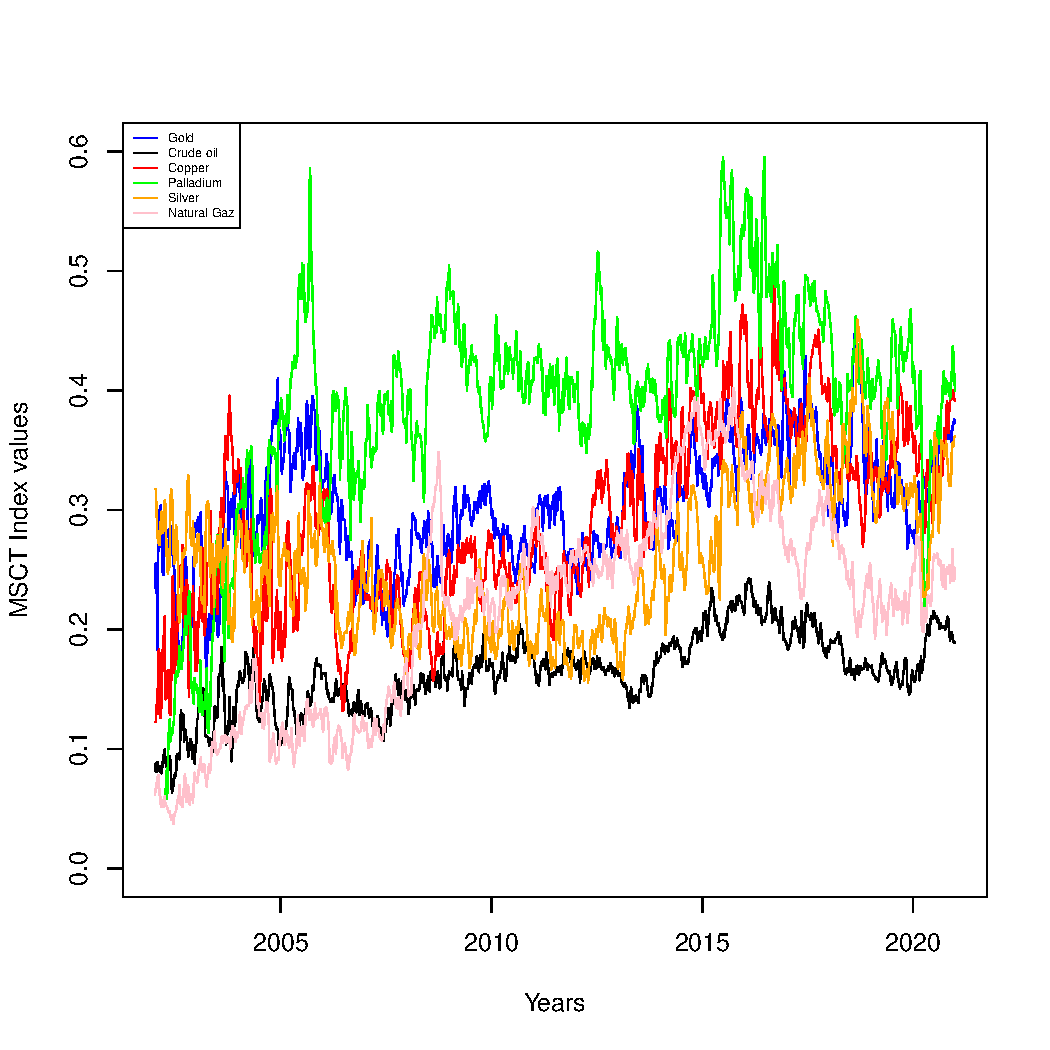
\includegraphics[scale=0.8]{FIG_MSCT}}
		\caption{Time series showing the evolution of the Market Share of Non-Commercials (MSCT) index for all commodities in our sample, 4/2007--12/2020. }
		\label{fig:MSCT}
	\end{figure}


	\begin{figure}[h]
	\centering
		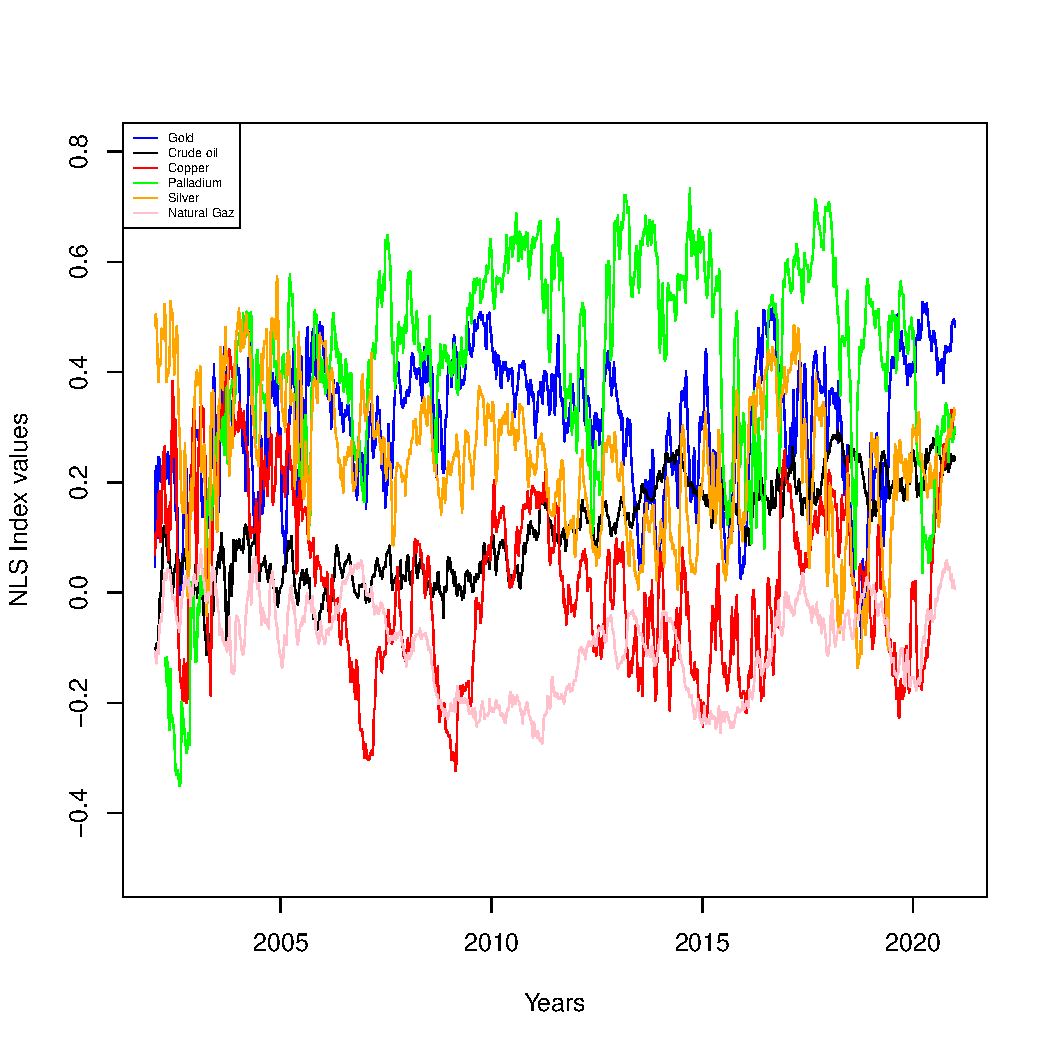
\includegraphics[scale=0.8]{FIG_NLS}}
		\caption{Time series showing the evolution of the Net Long Short (NLS) index for all commodities in our sample, 4/2007--12/2020.}
		\label{fig:NLS}
	\end{figure}

	\begin{figure}[h]
	\centering
		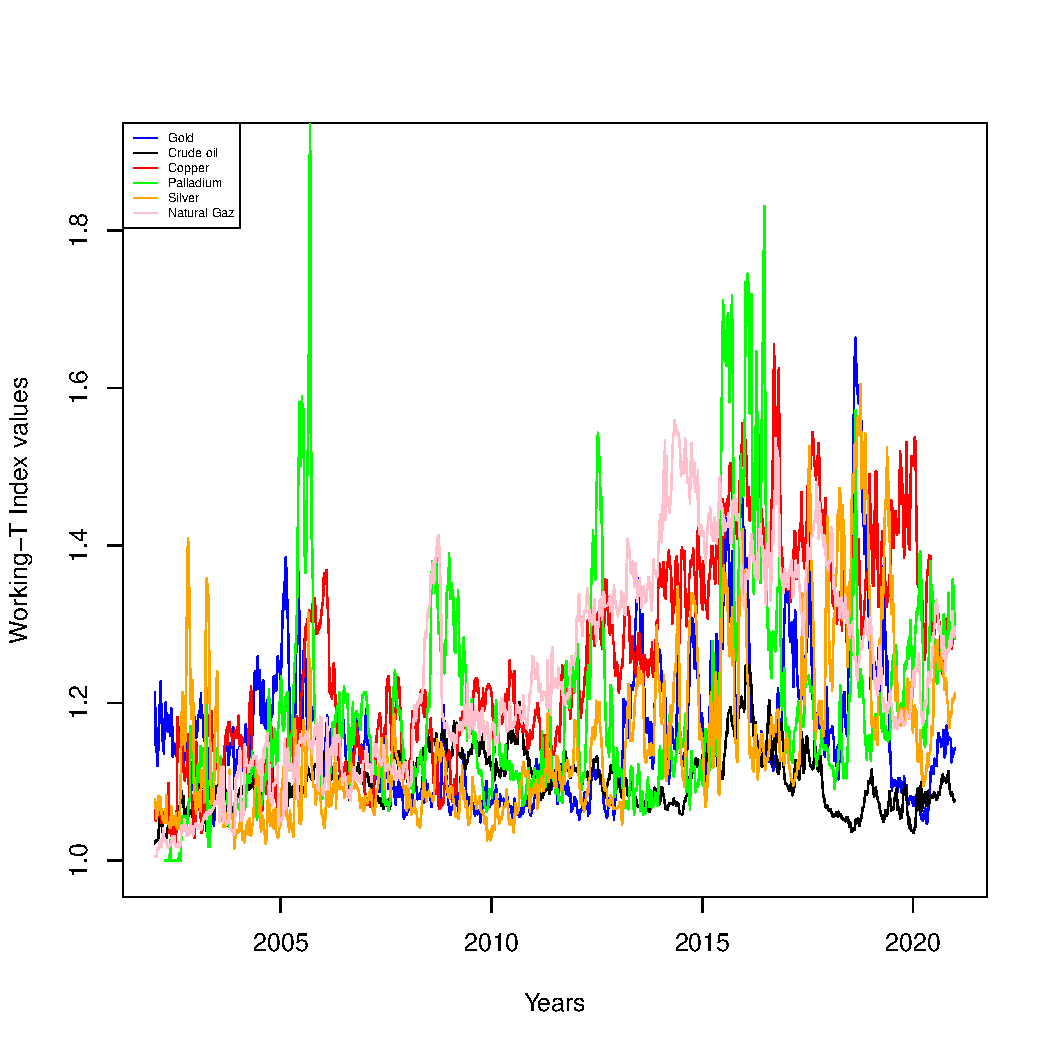
\includegraphics[scale=0.8]{FIG_WT}}
		\caption{Time series showing the evolution of the Working's T index for all commodities in our sample, 4/2007--12/2020.}
		\label{fig:WT}
	\end{figure}
	
%\documentclass[12pt]{article}
%
%\usepackage{amssymb,amsmath,amsfonts,eurosym,geometry,ulem,graphicx,caption,color,setspace,sectsty,comment,footmisc,caption,natbib,pdflscape,subfigure,array,hyperref}
%\usepackage{hyperref}
%\hypersetup{colorlinks,
%citecolor=blue,
%linkcolor=magenta
%}
%\usepackage{multirow}
%\usepackage{booktabs}
%\usepackage{graphicx}
%\usepackage{lscape}
%\usepackage{setspace}
%\usepackage{tabularx} 
%\usepackage{rotating}
%\usepackage{tablefootnote}
%\usepackage{amssymb}
%\usepackage{array}
%\usepackage{ragged2e}
%\usepackage{nicematrix}
%\usepackage{enumitem}
%\usepackage{array} 
%\usepackage{graphicx}
%\usepackage{booktabs}
%\usepackage{enumitem}
%\usepackage{wasysym}
%\usepackage{framed}
%\usepackage{pgfgantt}
%\usepackage{subfloat}
%\usepackage{multirow}
%\usepackage{blindtext}
%\usepackage{graphicx}
%\usepackage{lscape}
%\usepackage{colortbl}
%\usepackage{caption}
%\usepackage{threeparttable}
%\normalem
%
%\doublespacing
%\newtheorem{theorem}{Theorem}
%\newtheorem{corollary}[theorem]{Corollary}
%\newtheorem{proposition}{Proposition}
%\newenvironment{proof}[1][Proof]{\noindent\textbf{#1.} }{\ \rule{0.5em}{0.5em}}
%
%\newtheorem{hyp}{Hypothesis}
%\newtheorem{subhyp}{Hypothesis}[hyp]
%\renewcommand{\thesubhyp}{\thehyp\alph{subhyp}}
%\renewcommand{\familydefault}{\sfdefault} 
%
%
%\geometry{left=1.0in,right=1.0in,top=1.0in,bottom=1.0in}
%\bibliographystyle{aaai-named}
%
%\singlespacing
%\title{\textbf{Has financialization changed the impact\\ of macro announcements ?\\ Appendix A}\thanks{The authors thank participants at meetings of the Commodity \& Energy Markets Association (2021),  World Finance \& Banking Association (2021), Société canadienne de science  économique (2022), 4th Ethical Finance and Sustainability (EFS) conference (2022) as well as Alessandro Melone and Jocelyn Grira (discussants). For financial support, the authors thank the Social Sciences and Humanities Research Council and Chaire Industrielle-Alliance Groupe financier. Any remaining errors are ours alone.}}
%%J'arrive pas le centrer dans le titre
%\author{Simon-Pierre Boucher\footnote{Corresponding author, PhD student in finance, Université Laval, Quebec City QC Canada G1V 0A6, email:   \texttt{simon-pierre.boucher.1@ulaval.ca}}\and Marie-H{\'e}l{\`e}ne Gagnon\footnote{Professor of Finance and Research Fellow, CRREP, Université Laval, email: \texttt{marie-helene.gagnon@fsa.ulaval.ca}}\and Gabriel J. Power\footnote{Professor of Finance and Research Fellow, CRREP and CRIB, Université Laval, email:   \texttt{gabriel.power@fsa.ulaval.ca}}. 
%}
%%\author{ANONYMOUS VERSION}
%\date{ \today \\ First version: June 2021}
%\begin{document}
%\begin{titlepage}
%\maketitle
%
%
%
%
%
%\begin{abstract}
%\noindent 
%\singlespacing
%%Turmoil in commodity markets can threaten a sustainable energy future.
%%The transition to a sustainable energy future requires considerable investments, which can be discouraged by heightened volatility in commodity markets.
 %We investigate, using high-frequency data, how financialization has affected the impact of macroeconomic announcements on commodity futures returns and volatility. We find that financialization lessens the impact of macro news on commodity markets, as measured by price drift and volatility changes. This result is consistent with prior literature suggesting that financial participants improve liquidity and price discovery, while reducing volatility. Assuming that traditional market participants prefer stability, our results suggest a beneficial impact of financialization. We further show that the effects of greater participation by swap dealers and money managers differ.%, especially for pro-cyclical commodities such as crude oil and natural gas.
%
%\vspace{0.2in}
%\noindent\textbf{Keywords:} commodities, energy, futures,  spillover, financialization, high-frequency, sustainable, commercial, institutional, volatility, macro, announcements, surprise, events\\
%
%
%\bigskip
%\end{abstract}
%\setcounter{page}{0}
%\thispagestyle{empty}
%\end{titlepage}
%\pagebreak \newpage
%
%
%
%
%\doublespacing

\appendix{Appendix}
\section{Appendix: Full tables of results}
\begin{landscape}
\begin{table}[]
\caption{Announcement and financialization effects on futures returns}
\label{tab:appendix1}
\resizebox{\columnwidth}{!}{%
\begin{tabular}{lllllllllllll}
\hline
\textbf{Commodities} &
  \multicolumn{2}{c}{\textbf{Crude Oil}} &
  \multicolumn{2}{c}{\textbf{Gold}} &
  \multicolumn{2}{c}{\textbf{Copper}} &
  \multicolumn{2}{c}{\textbf{Silver}} &
  \multicolumn{2}{c}{\textbf{Palladium}} &
  \multicolumn{2}{c}{\textbf{Natural Gas}} \\ \hline
Announcements &
  $\gamma_m$ &
  $\theta_m$ &
  $\gamma_m$ &
  $\theta_m$ &
  $\gamma_m$ &
  $\theta_m$ &
  $\gamma_m$ &
  $\theta_m$ &
  $\gamma_m$ &
  $\theta_m$ &
  $\gamma_m$ &
  $\theta_m$ \\ \hline
Initial jobless claims   & -0.006    & 0.033     & -0.015*   & 0.051*    & -0.002   & 0.002     & -0.002    & 0.013     & 0.059***  & -0.141*** & -0.011   & 0.041   \\
ADP Employment           & 0.020***  & -0.092*** & -0.006*   & 0.016*    & 0.009*** & -0.029*** & 0.010***  & -0.038*** & 0.016***  & -0.043*** & -0.0005  & 0.001   \\
CB Consumer              & 0.0002    & 0.001     & 0.0004    & -0.002**  & 0.001*   & -0.001    & 0.0004    & -0.003*** & 0.0004    & -0.001    & 0.0003   & 0.00002 \\
Advance retail sales     & 0.005***  & -0.021*** & -0.002**  & 0.004     & 0.003*** & -0.010*** & 0.0002    & -0.002    & 0.001     & -0.002    & 0.002    & -0.010  \\
Building permit          & -0.002*** & 0.009***  & 0.001***  & -0.005*** & 0.001**  & -0.002**  & 0.001**   & -0.004*** & 0.001*    & -0.002**  & 0.001*   & -0.004* \\
Construction spending    & 0.002**   & -0.014**  & -0.001*   & 0.002     & 0.001    & -0.002    & 0.001     & -0.003*   & -0.001    & 0.002     & -0.00002 & -0.001  \\
Consumer\_credit         & -0.001    & 0.006     & 0.0001    & -0.0001   & 0.001**  & -0.002**  & 0.001***  & -0.002*** & 0.001**   & -0.002*   & -0.001*  & 0.004*  \\
Consumer price index     & -0.001    & 0.005     & 0.003***  & -0.011*** & 0.0002   & -0.0004   & 0.002***  & -0.009*** & -0.003*** & 0.005***  & -0.001   & 0.004   \\
Durable goods orders     & 0.002***  & -0.013*** & 0.004***  & -0.012*** & 0.003*** & -0.010*** & 0.003***  & -0.011*** & 0.001     & -0.001    & -0.001   & 0.002   \\
Existing home sales      & -0.001    & 0.006     & 0.0005    & -0.002    & 0.001*** & -0.002**  & 0.001*    & -0.002*   & 0.00002   & -0.0004   & 0.001    & -0.005  \\
Factory orders           & -0.003**  & 0.019**   & -0.001    & 0.002     & -0.001** & 0.004**   & -0.0001   & -0.001    & -0.001    & 0.001     & -0.002*  & 0.010** \\
GDP                      & 0.0003    & -0.0004   & -0.0002   & -0.002    & 0.002*** & -0.006*** & -0.002*** & 0.003*    & -0.001    & 0.001     & 0.0002   & -0.001  \\
Housing starts           & 0.001     & -0.004    & -0.0003   & -0.0002   & 0.001*** & -0.004*** & -0.002*** & 0.005***  & -0.003*** & 0.006***  & 0.001    & -0.003  \\
Industrial production    & 0.001     & -0.005    & -0.001    & 0.001     & 0.001    & -0.002    & -0.001**  & 0.003*    & 0.0003    & -0.001    & -0.0003  & 0.001   \\
Michigan Sentiment Index & 0.0002    & -0.0003   & -0.0003   & 0.0003    & 0.0001   & -0.0001   & -0.0003   & -0.0003   & -0.00002  & -0.0001   & -0.001   & 0.002   \\
New home sales           & 0.002     & -0.008    & 0.001     & -0.004**  & 0.002*** & -0.004*** & -0.001    & 0.001     & -0.0001   & 0.0005    & -0.001   & 0.004   \\
Non-farm employment      & 0.080***  & -0.384*** & -0.040*** & 0.117***  & 0.020*** & -0.064*** & 0.022***  & -0.081*** & 0.010***  & -0.027*** & -0.005   & 0.024   \\
Pending home sales       & 0.004***  & -0.021*** & -0.0003   & 0.001     & 0.0001   & 0.0003    & -0.0001   & 0.0002    & 0.001     & -0.002    & 0.0003   & 0.001   \\
Personal consumption     & 0.00003   & 0.00002   & 0.002***  & -0.007*** & 0.0005   & -0.001    & 0.0001    & 0.00005   & 0.002***  & -0.005*** & 0.001    & -0.003  \\
Personal income          & 0.010***  & -0.051*** & 0.001     & -0.002    & 0.003*** & -0.009*** & 0.002     & -0.010*   & 0.004***  & -0.011*** & 0.001    & -0.003  \\
Producer price index     & 0.002***  & -0.013*** & 0.002***  & -0.007*** & 0.001*** & -0.003*** & 0.002***  & -0.008*** & 0.001     & -0.003*   & 0.0002   & -0.001  \\
Trade balance            & 0.001     & -0.004    & -0.001    & 0.002     & 0.0001   & -0.0001   & -0.0005   & 0.002     & -0.0004   & 0.001     & -0.001   & 0.003   \\ \hline
$R^2$ &
  \multicolumn{2}{c}{0,001} &
  \multicolumn{2}{c}{0,001} &
  \multicolumn{2}{c}{0,0004} &
  \multicolumn{2}{c}{0,001} &
  \multicolumn{2}{c}{0,0004} &
  \multicolumn{2}{c}{0,0003} \\
Observations &
  \multicolumn{2}{c}{971,990} &
  \multicolumn{2}{c}{968,656} &
  \multicolumn{2}{c}{917,529} &
  \multicolumn{2}{c}{960,063} &
  \multicolumn{2}{c}{609,496} &
  \multicolumn{2}{c}{880,021} \\ \hline
\end{tabular}%
}
\singlespacing
        \footnotesize
 Presents the estimates of mean equation, using the method proposed by \citep{kurov2019price} and financialization variable $X_{t,1}=MSCT_t$. The $\gamma_m$ coefficients capture the instantaneous change in return when an announcement has just occurred and especially if that announcement was unanticipated. The coefficients $\theta_m$ capture the instantaneous change in return when an announcement has just occurred in conjunction with the level of financialization.
\end{table}
\end{landscape}

\begin{landscape}
\begin{table}[]
\caption{Announcement and financialization effects on futures returns}
\label{tab:appendix2}
\resizebox{\columnwidth}{!}{%
\begin{tabular}{lllllllllllll}
\hline
\textbf{Commodities} &
  \multicolumn{2}{c}{\textbf{Crude Oil}} &
  \multicolumn{2}{c}{\textbf{Gold}} &
  \multicolumn{2}{c}{\textbf{Copper}} &
  \multicolumn{2}{c}{\textbf{Silver}} &
  \multicolumn{2}{c}{\textbf{Palladium}} &
  \multicolumn{2}{c}{\textbf{Natural Gas}} \\ \hline
Announcements &
  $\gamma_m$ &
  $\theta_m$ &
  $\gamma_m$ &
  $\theta_m$ &
  $\gamma_m$ &
  $\theta_m$ &
  $\gamma_m$ &
  $\theta_m$ &
  $\gamma_m$ &
  $\theta_m$ &
  $\gamma_m$ &
  $\theta_m$ \\ \hline
Initial jobless claims   & 0.0004    & -0.009    & -0.004     & 0.012    & -0.001    & -0.002    & 0.001      & 0.008    & -0.014*   & 0.021     & -0.007*   & -0.036    \\
ADP Employment           & 0.007***  & -0.022*** & -0.015***  & 0.031*** & 0.0003*** & 0.0004    & -0.006***  & 0.026*** & 0.0002    & -0.003**  & -0.001*** & -0.025**  \\
CB Consumer              & 0.001***  & -0.005*** & -0.0004*** & 0.001**  & 0.0001*** & 0.001*    & -0.001***  & 0.001*   & -0.001*** & 0.001***  & 0.0004*   & 0.001     \\
Advance retail sales     & 0.002***  & -0.007*** & -0.004***  & 0.008*** & 0.0001**  & -0.002    & -0.001***  & 0.004**  & -0.0001   & 0.0003    & 0.00001   & -0.001    \\
Building permit          & -0.00004  & 0.0004    & -0.0004*** & 0.001*** & 0.00003   & -0.0003   & -0.0002    & 0.00001  & -0.0002   & -0.0001   & 0.001***  & 0.004**   \\
Construction spending    & 0.001**   & -0.005**  & -0.001***  & 0.002*** & 0.00004   & -0.002*** & -0.001***  & 0.003*** & 0.001*    & -0.001*   & -0.0002   & -0.00002  \\
Consumer\_credit         & -0.0001   & 0.001     & -0.0001    & 0.0003   & 0.00002   & 0.0003    & -0.0001    & 0.0005   & 0.001***  & -0.001*   & -0.0001   & -0.001    \\
Consumer price index     & -0.001*** & 0.003***  & -0.001***  & 0.003*** & -0.0001   & -0.002*** & -0.001***  & 0.003*** & 0.0002    & -0.001**  & 0.0002    & 0.002     \\
Durable goods orders     & 0.002***  & -0.008*** & -0.001***  & 0.001**  & 0.0001    & -0.00000  & -0.0002    & 0.0001   & 0.0003    & -0.00004  & -0.001**  & -0.005**  \\
Existing home sales      & 0.001***  & -0.006*** & -0.00001   & -0.00001 & 0.0002*** & -0.0005   & 0.00002    & 0.0002   & -0.0003   & 0.0003    & 0.0002    & 0.001     \\
Factory orders           & -0.001**  & 0.005***  & -0.001*    & 0.001    & 0.0001    & -0.001    & -0.001***  & 0.004*** & -0.001    & 0.001     & 0.001***  & 0.004     \\
GDP                      & 0.001**   & -0.003*   & -0.001***  & 0.001    & 0.0003*** & 0.0003    & -0.002***  & 0.003*** & -0.002*** & 0.002**   & -0.0002   & -0.003    \\
Housing starts           & 0.001*    & -0.003*   & -0.001***  & 0.001*** & 0.0001    & 0.001     & -0.001***  & 0.002**  & -0.001**  & 0.001**   & -0.0004*  & -0.001    \\
Industrial production    & 0.0003    & -0.001    & 0.0002     & -0.001*  & -0.00001  & 0.0002    & 0.00002    & -0.001   & -0.0004   & 0.001     & -0.0001   & -0.001    \\
Michigan Sentiment Index & 0.0004    & -0.001    & -0.0001    & -0.0003  & 0.00005   & 0.001     & -0.0004*** & 0.0004   & -0.001**  & 0.001*    & -0.0003   & -0.002    \\
New home sales           & 0.001**   & -0.003    & -0.001***  & 0.001**  & 0.0002*** & -0.001    & -0.0005*** & 0.0001   & -0.0003   & 0.001     & 0.0003    & 0.0002    \\
Non-farm employment      & 0.036***  & -0.136*** & -0.046***  & 0.100*** & -0.0001   & -0.006    & -0.009***  & 0.041*** & 0.0004    & -0.004    & -0.002*** & -0.071*** \\
Pending home sales       & 0.001***  & -0.005*** & -0.0002    & 0.0001   & 0.0002**  & -0.001    & 0.00001    & -0.0003  & -0.00002  & 0.0003    & -0.0002   & -0.006*   \\
Personal consumption     & 0.0003    & -0.001    & -0.0003*   & 0.001    & 0.0001    & 0.001     & 0.0002     & -0.001   & 0.001***  & -0.001*** & 0.0001    & 0.002     \\
Personal income          & 0.006***  & -0.025*** & -0.008***  & 0.016*** & -0.0002*  & -0.001    & -0.002***  & 0.009*** & 0.0005*   & -0.002*** & -0.0004   & -0.009**  \\
Producer price index     & 0.001***  & -0.003*** & -0.001***  & 0.002*** & 0.00005   & -0.00000  & -0.0003    & 0.001    & -0.001*** & 0.002***  & -0.0004   & -0.002    \\
Trade balance            & -0.0004   & 0.002     & -0.001***  & 0.002*** & 0.00003   & -0.001**  & -0.001**   & 0.003*** & 0.001**   & -0.002**  & 0.0001    & 0.001     \\ \hline
$R^2$ &
  \multicolumn{2}{c}{0,001} &
  \multicolumn{2}{c}{0,002} &
  \multicolumn{2}{c}{0,0003} &
  \multicolumn{2}{c}{0,001} &
  \multicolumn{2}{c}{0,0003} &
  \multicolumn{2}{c}{0,0003} \\
Observations &
  \multicolumn{2}{c}{971,990} &
  \multicolumn{2}{c}{968,656} &
  \multicolumn{2}{c}{917,529} &
  \multicolumn{2}{c}{960,063} &
  \multicolumn{2}{c}{609,496} &
  \multicolumn{2}{c}{880,021} \\ \hline
\end{tabular}%
}
\singlespacing
        \footnotesize
 Presents the estimates of mean equation, using the method proposed by \citep{kurov2019price} and financialization variable $X_{t,2}=NLS_t$. The $\gamma_m$ coefficients capture the instantaneous change in return when an announcement has just occurred and especially if that announcement was unanticipated. The coefficients $\theta_m$ capture the instantaneous change in return when an announcement has just occurred in conjunction with the level of financialization.
\end{table}
\end{landscape}


\begin{landscape}
\begin{table}[]
\caption{Announcement and financialization effects on futures returns}
\label{tab:appendix3}
\resizebox{\columnwidth}{!}{%
\begin{tabular}{lllllllllllll}
\hline
\textbf{Commodities} &
  \multicolumn{2}{c}{\textbf{Crude Oil}} &
  \multicolumn{2}{c}{\textbf{Gold}} &
  \multicolumn{2}{c}{\textbf{Copper}} &
  \multicolumn{2}{c}{\textbf{Silver}} &
  \multicolumn{2}{c}{\textbf{Palladium}} &
  \multicolumn{2}{c}{\textbf{Natural Gas}} \\ \hline
Announcements &
  $\gamma_m$ &
  $\theta_m$ &
  $\gamma_m$ &
  $\theta_m$ &
  $\gamma_m$ &
  $\theta_m$ &
  $\gamma_m$ &
  $\theta_m$ &
  $\gamma_m$ &
  $\theta_m$ &
  $\gamma_m$ &
  $\theta_m$ \\ \hline
Initial jobless claims &
  -0.072 &
  0.065 &
  0.012 &
  -0.010 &
  -0.004 &
  0.002 &
  -0.004 &
  0.005 &
  0.060*** &
  -0.050*** &
  -0.026 &
  0.020 \\
ADP Employment &
  -0.002 &
  0.002 &
  0.022*** &
  -0.020*** &
  0.018*** &
  -0.013*** &
  0.035*** &
  -0.031*** &
  -0.005 &
  0.003 &
  0.005 &
  -0.004 \\
CB Consumer &
  -0.006** &
  0.005** &
  0.001* &
  -0.001*** &
  0.002*** &
  -0.002*** &
  0.002*** &
  -0.002*** &
  0.002** &
  -0.001** &
  -0.0005 &
  0.001 \\
Advance retail sales &
  -0.015** &
  0.014** &
  0.006*** &
  -0.006*** &
  0.009*** &
  -0.007*** &
  0.007*** &
  -0.007*** &
  0.001 &
  -0.001 &
  -0.001 &
  0.001 \\
Building permit &
  -0.004** &
  0.004** &
  0.001*** &
  -0.001*** &
  0.001 &
  -0.001 &
  0.001 &
  -0.001 &
  0.001* &
  -0.001** &
  0.002 &
  -0.002 \\
Construction spending &
  -0.002 &
  0.002 &
  0.001 &
  -0.001 &
  0.002 &
  -0.001 &
  0.003*** &
  -0.002*** &
  -0.002* &
  0.002* &
  -0.001 &
  0.0004 \\
Consumer\_credit &
  0.001 &
  -0.001 &
  0.0002 &
  -0.0002 &
  0.001* &
  -0.001* &
  0.001*** &
  -0.001*** &
  0.00003 &
  0.0002 &
  -0.002 &
  0.001 \\
Consumer price index &
  0.006** &
  -0.006** &
  0.005*** &
  -0.005*** &
  0.001 &
  -0.001 &
  0.010*** &
  -0.009*** &
  -0.003*** &
  0.002*** &
  -0.004* &
  0.003* \\
Durable goods orders &
  -0.004 &
  0.004 &
  0.005*** &
  -0.004*** &
  0.007*** &
  -0.005*** &
  0.005*** &
  -0.004*** &
  0.001 &
  -0.0003 &
  0.001 &
  -0.0004 \\
Existing home sales &
  -0.009*** &
  0.008*** &
  -0.00001 &
  -0.00001 &
  0.002*** &
  -0.001** &
  0.001 &
  -0.001 &
  0.0002 &
  -0.0002 &
  0.002 &
  -0.002 \\
Factory orders &
  0.005 &
  -0.004 &
  0.0001 &
  -0.0002 &
  -0.003*** &
  0.003*** &
  0.003** &
  -0.003** &
  0.001 &
  -0.001 &
  -0.007*** &
  0.006*** \\
GDP &
  -0.004 &
  0.004 &
  -0.0003 &
  -0.0005 &
  0.003** &
  -0.002* &
  0.0002 &
  -0.001 &
  0.001 &
  -0.001 &
  0.001 &
  -0.0004 \\
Housing starts &
  0.0003 &
  -0.0002 &
  0.001 &
  -0.001* &
  0.003*** &
  -0.002*** &
  -0.002* &
  0.001 &
  -0.001 &
  0.0005 &
  0.002 &
  -0.002 \\
Industrial production &
  -0.0003 &
  0.0004 &
  -0.002** &
  0.001** &
  0.001 &
  -0.001 &
  -0.004*** &
  0.003*** &
  0.001 &
  -0.001 &
  0.001 &
  -0.0005 \\
Michigan Sentiment Index &
  -0.001 &
  0.001 &
  -0.001 &
  0.0004 &
  0.0005 &
  -0.0003 &
  -0.0001 &
  -0.0002 &
  0.001 &
  -0.001 &
  -0.001 &
  0.001 \\
New home sales &
  0.002 &
  -0.002 &
  0.001 &
  -0.001** &
  0.005*** &
  -0.003*** &
  -0.001 &
  0.001 &
  0.001 &
  -0.001 &
  -0.001 &
  0.001 \\
Non-farm employment &
  -0.231*** &
  0.214*** &
  0.073*** &
  -0.066*** &
  0.095*** &
  -0.069*** &
  0.094*** &
  -0.082*** &
  0.005 &
  -0.004 &
  0.017 &
  -0.013 \\
Pending home sales &
  -0.007 &
  0.007 &
  -0.0001 &
  -0.00005 &
  0.001 &
  -0.001 &
  -0.0001 &
  -0.00000 &
  0.001 &
  -0.001 &
  0.001 &
  -0.0003 \\
Personal consumption &
  -0.0004 &
  0.0004 &
  0.003*** &
  -0.002*** &
  0.002 &
  -0.001 &
  -0.0002 &
  0.0003 &
  -0.003** &
  0.002*** &
  0.0001 &
  -0.0002 \\
Personal income &
  -0.040*** &
  0.037*** &
  0.017*** &
  -0.016*** &
  0.021*** &
  -0.016*** &
  0.019*** &
  -0.017*** &
  0.004** &
  -0.003** &
  0.008* &
  -0.006* \\
Producer price index &
  -0.003 &
  0.003 &
  0.003*** &
  -0.003*** &
  0.002** &
  -0.002** &
  0.004*** &
  -0.004*** &
  0.003*** &
  -0.003*** &
  0.002 &
  -0.002 \\
Trade balance &
  0.005* &
  -0.005* &
  0.001 &
  -0.001 &
  -0.001 &
  0.001 &
  0.0004 &
  -0.0003 &
  -0.002* &
  0.002* &
  -0.003 &
  0.002 \\ \hline
$R^2$ &
  \multicolumn{2}{c}{0,001} &
  \multicolumn{2}{c}{0,002} &
  \multicolumn{2}{c}{0,001} &
  \multicolumn{2}{c}{0,001} &
  \multicolumn{2}{c}{0,0004} &
  \multicolumn{2}{c}{0,0003} \\
Observations &
  \multicolumn{2}{c}{971,990} &
  \multicolumn{2}{c}{968,656} &
  \multicolumn{2}{c}{917,529} &
  \multicolumn{2}{c}{960,063} &
  \multicolumn{2}{c}{609,496} &
  \multicolumn{2}{c}{880,021} \\ \hline
\end{tabular}%
}
\singlespacing
        \footnotesize
 Presents the estimates of mean equation, using the method proposed by \citep{kurov2019price} and financialization variable $X_{t,3}=WORKINGTS_t$. The $\gamma_m$ coefficients capture the instantaneous change in return when an announcement has just occurred and especially if that announcement was unanticipated. The coefficients $\theta_m$ capture the instantaneous change in return when an announcement has just occurred in conjunction with the level of financialization.
\end{table}
\end{landscape}

\begin{landscape}
\begin{table}[]
\caption{Announcement and financialization effects on futures returns}
\label{tab:appendix4}
\resizebox{\columnwidth}{!}{%
\begin{tabular}{lllllllllllll}
\hline
\textbf{Commodities} &
  \multicolumn{2}{c}{\textbf{Crude Oil}} &
  \multicolumn{2}{c}{\textbf{Gold}} &
  \multicolumn{2}{c}{\textbf{Copper}} &
  \multicolumn{2}{c}{\textbf{Silver}} &
  \multicolumn{2}{c}{\textbf{Palladium}} &
  \multicolumn{2}{c}{\textbf{Natural Gas}} \\ \hline
Announcements &
  $\gamma_m$ &
  $\theta_m$ &
  $\gamma_m$ &
  $\theta_m$ &
  $\gamma_m$ &
  $\theta_m$ &
  $\gamma_m$ &
  $\theta_m$ &
  $\gamma_m$ &
  $\theta_m$ &
  $\gamma_m$ &
  $\theta_m$ \\ \hline
Initial jobless claims   & -0.034   & 0.183     & -0.018    & 0.062     & -0.001    & 0.0004    & -0.006   & 0.027     & 0.064**  & -0.149**  & -0.015   & 0.064   \\
ADP Employment           & 0.028**  & -0.131**  & -0.007    & 0.019     & 0.004     & -0.013    & 0.008**  & -0.033*** & 0.017**  & -0.046**  & -0.005   & 0.023   \\
CB Consumer              & 0.002    & -0.010    & 0.0004    & -0.002*   & 0.001***  & -0.002*   & 0.001    & -0.003**  & 0.001    & -0.003    & -0.0003  & 0.003   \\
Advance retail sales     & 0.009*** & -0.041*** & -0.003**  & 0.006     & 0.006***  & -0.019*** & 0.0004   & -0.002    & 0.002    & -0.005    & 0.002    & -0.009  \\
Building permit          & -0.001   & 0.007     & 0.002***  & -0.007*** & 0.001**   & -0.004**  & 0.001    & -0.004    & 0.001**  & -0.003*** & 0.001    & -0.003  \\
Construction spending    & 0.002    & -0.014*   & 0.00003   & -0.001    & 0.001**   & -0.004*   & 0.0005   & -0.003    & 0.0005   & -0.001    & 0.001    & -0.005  \\
Consumer\_credit         & 0.001    & -0.005    & 0.0005*   & -0.001    & 0.001**   & -0.002*   & 0.001*** & -0.004*** & 0.0001   & -0.0001   & -0.001*  & 0.004*  \\
Consumer price index     & -0.002   & 0.007     & 0.003***  & -0.010*** & -0.00004  & 0.0004    & 0.001    & -0.006*   & -0.001   & 0.001     & -0.001   & 0.005   \\
Durable goods orders     & 0.003*   & -0.019*   & 0.005***  & -0.016*** & 0.004***  & -0.010*** & 0.003*** & -0.013*** & 0.00005  & 0.001     & -0.001   & 0.001   \\
Existing home sales      & 0.0005   & 0.0002    & 0.001***  & -0.004*** & 0.001***  & -0.003*** & 0.001*** & -0.003*** & 0.001    & -0.004    & 0.001    & -0.003  \\
Factory orders           & -0.001*  & 0.006**   & -0.001*** & 0.003**   & -0.002*** & 0.008***  & -0.001   & 0.002     & 0.001    & -0.002    & -0.003** & 0.013** \\
GDP                      & 0.001    & -0.005    & 0.003***  & -0.011*** & 0.002**   & -0.005*   & -0.001   & 0.001     & -0.002   & 0.004     & -0.0002  & 0.001   \\
Housing starts           & 0.001    & -0.005    & -0.001    & 0.001     & 0.002*    & -0.004*   & -0.002** & 0.005*    & -0.002** & 0.005*    & 0.001    & -0.003  \\
Industrial production    & 0.001    & -0.003    & -0.001    & 0.001     & 0.00003   & -0.0003   & -0.001   & 0.002     & -0.002*  & 0.004*    & 0.001    & -0.003  \\
Michigan Sentiment Index & 0.001    & -0.006    & 0.0002    & -0.001    & 0.001     & -0.001    & 0.0002   & -0.002    & 0.001    & -0.002    & -0.001   & 0.003   \\
New home sales           & 0.002    & -0.007    & 0.001     & -0.004    & 0.003***  & -0.007*** & 0.0001   & -0.003    & 0.0004   & -0.001    & -0.001   & 0.004   \\
Non-farm employment      & 0.093*** & -0.443*** & -0.014*** & 0.040***  & 0.027***  & -0.088*** & 0.014**  & -0.051**  & 0.002    & -0.005    & -0.014   & 0.062   \\
Pending home sales       & 0.003*   & -0.015*   & -0.001    & 0.003     & 0.001     & -0.003    & -0.0002  & 0.001     & 0.001    & -0.004    & 0.002    & -0.007  \\
Personal consumption     & 0.001    & -0.004    & 0.002     & -0.007*   & 0.001     & -0.002    & -0.0002  & 0.0004    & -0.00000 & 0.001     & -0.001   & 0.004   \\
Personal income          & 0.019*** & -0.092*** & 0.0001    & 0.0001    & 0.004**   & -0.012**  & -0.001   & 0.011     & 0.003*** & -0.008*** & -0.0001  & 0.001   \\
Producer price index     & 0.002    & -0.014    & 0.002**   & -0.007*** & 0.001**   & -0.003*   & 0.002*** & -0.011*** & 0.001    & -0.003    & 0.0002   & -0.0004 \\
Trade balance            & 0.002    & -0.010    & 0.001     & -0.003*   & 0.0003    & -0.001    & -0.0003  & -0.0003   & -0.007** & 0.015**   & -0.002   & 0.007   \\ \hline
$R^2$ &
  \multicolumn{2}{c}{0,021} &
  \multicolumn{2}{c}{0,001} &
  \multicolumn{2}{c}{0,0003} &
  \multicolumn{2}{c}{0,001} &
  \multicolumn{2}{c}{0,0004} &
  \multicolumn{2}{c}{0,0004} \\
Observations &
  \multicolumn{2}{c}{971,990} &
  \multicolumn{2}{c}{968,656} &
  \multicolumn{2}{c}{917,529} &
  \multicolumn{2}{c}{960,063} &
  \multicolumn{2}{c}{609,496} &
  \multicolumn{2}{c}{880,021} \\ \hline
\end{tabular}%
}
\singlespacing
        \footnotesize
 Presents the estimates of mean equation, using the method proposed by \citep{andersen2007real} and financialization variable $X_{t,1}=MSCT_t$. The $\gamma_m$ coefficients capture the instantaneous change in return when an announcement has just occurred and especially if that announcement was unanticipated. The coefficients $\theta_m$ capture the instantaneous change in return when an announcement has just occurred in conjunction with the level of financialization.
\end{table}
\end{landscape}

\begin{landscape}
\begin{table}[]
\caption{Announcement and financialization effects on futures returns}
\label{tab:appendix5}
\resizebox{\columnwidth}{!}{%
\begin{tabular}{lllllllllllll}
\hline
\textbf{Commodities} &
  \multicolumn{2}{c}{\textbf{Crude Oil}} &
  \multicolumn{2}{c}{\textbf{Gold}} &
  \multicolumn{2}{c}{\textbf{Copper}} &
  \multicolumn{2}{c}{\textbf{Silver}} &
  \multicolumn{2}{c}{\textbf{Palladium}} &
  \multicolumn{2}{c}{\textbf{Natural Gas}} \\ \hline
Announcements &
  $\gamma_m$ &
  $\theta_m$ &
  $\gamma_m$ &
  $\theta_m$ &
  $\gamma_m$ &
  $\theta_m$ &
  $\gamma_m$ &
  $\theta_m$ &
  $\gamma_m$ &
  $\theta_m$ &
  $\gamma_m$ &
  $\theta_m$ \\ \hline
Initial jobless claims &
  -0.004 &
  0.014 &
  -0.003 &
  0.010 &
  -0.0003 &
  -0.003 &
  0.0003 &
  0.008 &
  -0.005 &
  0.014 &
  -0.005 &
  -0.028 \\
ADP Employment &
  0.010*** &
  -0.034** &
  -0.015*** &
  0.033*** &
  0.0003*** &
  -0.001 &
  -0.009*** &
  0.036*** &
  0.0002 &
  -0.004 &
  -0.001 &
  -0.018 \\
CB Consumer &
  0.001*** &
  -0.007*** &
  -0.001*** &
  0.001*** &
  0.0003*** &
  0.0001 &
  -0.001*** &
  0.002** &
  -0.001* &
  0.002** &
  0.0004 &
  0.001 \\
Advance retail sales &
  0.003*** &
  -0.008*** &
  -0.004*** &
  0.007*** &
  0.0003*** &
  -0.005*** &
  -0.001 &
  0.003 &
  0.0001 &
  -0.001 &
  0.00000 &
  -0.001 \\
Building permit &
  0.001 &
  -0.002 &
  -0.00004 &
  0.0003 &
  -0.00004 &
  -0.0002 &
  0.00003 &
  -0.001 &
  0.001* &
  -0.002** &
  0.001* &
  0.006* \\
Construction spending &
  0.0004 &
  -0.004* &
  -0.0001 &
  -0.0003 &
  0.0001 &
  -0.003*** &
  -0.001 &
  0.002 &
  0.001 &
  -0.001 &
  -0.0002 &
  -0.002 \\
Consumer\_credit &
  0.0004*** &
  -0.002*** &
  0.0002 &
  -0.0002 &
  0.0001 &
  -0.0003 &
  -0.00003 &
  0.0004 &
  0.0005 &
  -0.001 &
  0.0003 &
  0.001 \\
Consumer price index &
  -0.001** &
  0.003 &
  -0.002*** &
  0.004*** &
  -0.0001 &
  -0.002** &
  -0.001*** &
  0.002*** &
  0.001 &
  -0.002 &
  0.0002 &
  0.003 \\
Durable goods orders &
  0.001** &
  -0.007** &
  -0.001** &
  0.002** &
  0.0002 &
  -0.001 &
  -0.001** &
  0.004** &
  0.0004 &
  -0.0001 &
  -0.001* &
  -0.005* \\
Existing home sales &
  0.001*** &
  -0.002 &
  0.0001 &
  0.0003 &
  0.0004*** &
  -0.002* &
  0.001*** &
  -0.0004 &
  -0.00002 &
  -0.001 &
  -0.0002 &
  -0.001 \\
Factory orders &
  -0.0004 &
  0.004* &
  -0.001*** &
  0.003*** &
  -0.0001 &
  -0.0002 &
  -0.001** &
  0.004** &
  -0.0002 &
  0.0002 &
  0.002*** &
  0.011*** \\
GDP &
  0.001** &
  -0.005* &
  -0.001*** &
  0.002*** &
  0.0004*** &
  -0.0001 &
  -0.002*** &
  0.006*** &
  -0.001 &
  0.002 &
  -0.001 &
  -0.005 \\
Housing starts &
  0.001 &
  -0.005 &
  -0.001*** &
  0.001 &
  0.0001 &
  0.001 &
  -0.001** &
  0.001 &
  -0.002*** &
  0.004*** &
  -0.0004 &
  -0.002 \\
Industrial production &
  0.0001 &
  -0.001 &
  -0.0001 &
  -0.001 &
  -0.00002 &
  0.001 &
  0.00001 &
  -0.002 &
  -0.001* &
  0.001* &
  0.00004 &
  0.0002 \\
Michigan Sentiment Index &
  0.0005 &
  -0.002 &
  -0.0002 &
  0.0001 &
  0.0001 &
  0.001 &
  -0.001* &
  0.001 &
  -0.001** &
  0.002** &
  -0.0004 &
  -0.003 \\
New home sales &
  0.002*** &
  -0.008*** &
  -0.001** &
  0.001 &
  0.0003*** &
  -0.001 &
  -0.001** &
  0.001 &
  -0.001 &
  0.001 &
  0.0002 &
  0.001 \\
Non-farm employment &
  0.036*** &
  -0.135*** &
  -0.040*** &
  0.086*** &
  -0.0001*** &
  -0.006 &
  -0.002 &
  0.009 &
  -0.00005 &
  0.004 &
  -0.004*** &
  -0.129*** \\
Pending home sales &
  0.001** &
  -0.004* &
  -0.001 &
  0.001 &
  -0.00001 &
  -0.003*** &
  0.0001 &
  -0.0003 &
  0.0001 &
  -0.001 &
  -0.0005 &
  -0.005** \\
Personal consumption &
  0.0002 &
  -0.002 &
  -0.0004 &
  0.001 &
  0.0001 &
  0.002 &
  0.0001 &
  -0.001 &
  0.00005 &
  0.001 &
  -0.0003 &
  -0.003 \\
Personal income &
  0.009*** &
  -0.036*** &
  -0.007*** &
  0.016*** &
  -0.0004* &
  -0.003* &
  -0.0001 &
  0.002 &
  0.001*** &
  -0.003** &
  -0.0002 &
  -0.009 \\
Producer price index &
  0.0004 &
  -0.003 &
  -0.001*** &
  0.002*** &
  0.0003** &
  0.0005 &
  0.0001 &
  -0.001 &
  -0.004*** &
  0.007*** &
  0.00005 &
  -0.0001 \\
Trade balance &
  -0.001 &
  0.004 &
  -0.001*** &
  0.003*** &
  0.00001 &
  -0.002* &
  -0.001** &
  0.006*** &
  0.002* &
  -0.003* &
  0.001 &
  0.006 \\ \hline
$R^2$ &
  \multicolumn{2}{c}{0,021} &
  \multicolumn{2}{c}{0,014} &
  \multicolumn{2}{c}{0,0003} &
  \multicolumn{2}{c}{0,001} &
  \multicolumn{2}{c}{0,183} &
  \multicolumn{2}{c}{0,017} \\
Observations &
  \multicolumn{2}{c}{971,990} &
  \multicolumn{2}{c}{968,656} &
  \multicolumn{2}{c}{917,529} &
  \multicolumn{2}{c}{960,063} &
  \multicolumn{2}{c}{609,496} &
  \multicolumn{2}{c}{880,021} \\ \hline
\end{tabular}%
}
\singlespacing
        \footnotesize
 Presents the estimates of mean equation, using the method proposed by \citep{andersen2007real} and financialization variable $X_{t,2}=NLS_t$. The $\gamma_m$ coefficients capture the instantaneous change in return when an announcement has just occurred and especially if that announcement was unanticipated. The coefficients $\theta_m$ capture the instantaneous change in return when an announcement has just occurred in conjunction with the level of financialization.
\end{table}
\end{landscape}

\begin{landscape}
\begin{table}[]
\caption{Announcement and financialization effects on futures returns}
\label{tab:appendix6}
\resizebox{\columnwidth}{!}{%
\begin{tabular}{lllllllllllll}
\hline
\textbf{Commodities} &
  \multicolumn{2}{c}{\textbf{Crude Oil}} &
  \multicolumn{2}{c}{\textbf{Gold}} &
  \multicolumn{2}{c}{\textbf{Copper}} &
  \multicolumn{2}{c}{\textbf{Silver}} &
  \multicolumn{2}{c}{\textbf{Palladium}} &
  \multicolumn{2}{c}{\textbf{Natural Gas}} \\ \hline
Announcements &
  $\gamma_m$ &
  $\theta_m$ &
  $\gamma_m$ &
  $\theta_m$ &
  $\gamma_m$ &
  $\theta_m$ &
  $\gamma_m$ &
  $\theta_m$ &
  $\gamma_m$ &
  $\theta_m$ &
  $\gamma_m$ &
  $\theta_m$ \\ \hline
Initial jobless claims   & 0.011     & -0.011   & 0.005    & -0.004    & -0.003    & 0.001     & -0.008    & 0.008     & 0.077**  & -0.063**  & -0.034    & 0.028    \\
ADP Employment           & -0.066    & 0.062    & 0.022*** & -0.020*** & 0.017**   & -0.012**  & 0.034***  & -0.030*** & -0.004   & 0.003     & -0.016    & 0.013    \\
CB Consumer              & -0.004    & 0.004    & 0.001**  & -0.001*** & 0.003***  & -0.002*** & 0.003***  & -0.003*** & 0.003**  & -0.002**  & -0.001    & 0.001    \\
Advance retail sales     & -0.014    & 0.013    & 0.004*   & -0.004**  & 0.016***  & -0.012*** & 0.011***  & -0.010*** & -0.001   & 0.0003    & 0.002     & -0.001   \\
Building permit          & -0.007    & 0.006    & 0.002**  & -0.001**  & 0.001     & -0.001    & 0.001     & -0.001    & 0.001    & -0.001    & -0.00004  & 0.0002   \\
Construction spending    & -0.003    & 0.002    & 0.001*   & -0.001**  & 0.003**   & -0.002*   & 0.002     & -0.001    & -0.001   & 0.001     & 0.004     & -0.003   \\
Consumer\_credit         & -0.007*** & 0.007*** & 0.00003  & 0.00002   & 0.001     & -0.001    & 0.002**   & -0.002**  & -0.001   & 0.001     & -0.003**  & 0.003**  \\
Consumer price index     & 0.006     & -0.006   & 0.006*** & -0.005*** & 0.001     & -0.001    & 0.007***  & -0.007*** & -0.003   & 0.002     & -0.005    & 0.003    \\
Durable goods orders     & -0.003    & 0.003    & 0.009*** & -0.008*** & 0.008***  & -0.006*** & 0.009***  & -0.008*** & 0.0002   & 0.0001    & 0.001     & -0.001   \\
Existing home sales      & -0.003    & 0.003    & 0.001    & -0.001    & 0.002**   & -0.001**  & 0.002**   & -0.001*   & 0.0002   & -0.0004   & 0.002     & -0.002   \\
Factory orders           & 0.001     & -0.0004  & 0.001    & -0.001    & -0.005*** & 0.004***  & 0.002     & -0.002    & 0.0002   & -0.0002   & -0.013*** & 0.010*** \\
GDP                      & -0.004    & 0.004    & 0.003*** & -0.003*** & 0.002     & -0.002    & 0.006**   & -0.006**  & 0.001    & -0.001    & 0.0003    & -0.0001  \\
Housing starts           & -0.003    & 0.003    & 0.0004   & -0.001    & 0.003**   & -0.002*   & -0.003    & 0.002     & 0.0004   & -0.001    & 0.003     & -0.002   \\
Industrial production    & 0.004     & -0.003   & -0.002   & 0.001     & 0.0001    & -0.0001   & -0.004    & 0.003     & 0.001    & -0.001    & 0.004     & -0.003   \\
Michigan Sentiment Index & 0.002     & -0.002   & 0.00002  & -0.0002   & 0.001     & -0.001    & 0.001     & -0.002    & 0.003*   & -0.003**  & -0.001    & 0.001    \\
New home sales           & -0.013*   & 0.012**  & 0.001    & -0.001    & 0.007***  & -0.005*** & 0.001     & -0.001    & 0.002    & -0.002    & -0.002    & 0.001    \\
Non-farm employment      & -0.293*** & 0.271*** & 0.069*** & -0.063*** & 0.086***  & -0.062*** & 0.098***  & -0.086*** & 0.006    & -0.004    & 0.031     & -0.025   \\
Pending home sales       & -0.011    & 0.010    & 0.0004   & -0.0004   & 0.001     & -0.001    & -0.001    & 0.001     & 0.0003   & -0.0004   & 0.004     & -0.003   \\
Personal consumption     & 0.001     & -0.001   & 0.003    & -0.002    & 0.002     & -0.001    & -0.001    & 0.0005    & 0.001    & -0.0002   & -0.003    & 0.002    \\
Personal income          & -0.049*** & 0.045*** & 0.017*** & -0.014*** & 0.020***  & -0.015*** & -0.013*** & 0.012***  & 0.006*   & -0.004    & 0.005     & -0.004   \\
Producer price index     & -0.0003   & 0.0003   & 0.004*** & -0.004*** & 0.002     & -0.001    & 0.005**   & -0.005**  & 0.006*** & -0.006*** & 0.002     & -0.001   \\
Trade balance            & 0.008     & -0.007   & 0.002*** & -0.002*** & 0.0002    & -0.0001   & -0.0002   & -0.00002  & -0.006** & 0.005**   & -0.007**  & 0.005**  \\ \hline
$R^2$ &
  \multicolumn{2}{c}{0,005} &
  \multicolumn{2}{c}{0,001} &
  \multicolumn{2}{c}{0,0003} &
  \multicolumn{2}{c}{0,001} &
  \multicolumn{2}{c}{0,0002} &
  \multicolumn{2}{c}{0,0005} \\
Observations &
  \multicolumn{2}{c}{971,990} &
  \multicolumn{2}{c}{968,656} &
  \multicolumn{2}{c}{917,529} &
  \multicolumn{2}{c}{960,063} &
  \multicolumn{2}{c}{609,496} &
  \multicolumn{2}{c}{880,021} \\ \hline
\end{tabular}%
}
\singlespacing
        \footnotesize
 Presents the estimates of mean equation, using the method proposed by \citep{andersen2007real} and financialization variable $X_{t,3}=WORKINGT_t$. The $\gamma_m$ coefficients capture the instantaneous change in return when an announcement has just occurred and especially if that announcement was unanticipated. The coefficients $\theta_m$ capture the instantaneous change in return when an announcement has just occurred in conjunction with the level of financialization.
\end{table}
\end{landscape}

\begin{landscape}
\begin{table}[]
\caption{Announcement and financialization effects on futures conditional variance}
\label{tab:appendix7}
\resizebox{\columnwidth}{!}{%
\begin{tabular}{lllllllllllll}
\hline
\textbf{\textbackslash{}textbf\{Commodities\}} &
  \multicolumn{2}{c}{\textbf{Crude Oil}} &
  \multicolumn{2}{c}{\textbf{Gold}} &
  \multicolumn{2}{c}{\textbf{Copper}} &
  \multicolumn{2}{c}{\textbf{Silver}} &
  \multicolumn{2}{c}{\textbf{Palladium}} &
  \multicolumn{2}{c}{\textbf{Natural Gas}} \\ \hline
Announcements            & $\Phi_m$ & $\phi_m$  & $\Phi_m$  & $\phi_m$  & $\Phi_m$ & $\phi_m$  & $\Phi_m$  & $\phi_m$  & $\Phi_m$  & $\phi_m$  & $\Phi_m$ & $\phi_m$  \\ \hline
Initial jobless claims   & 0.004    & -0.024    & 0.001     & -0.005*   & -0.001   & 0.001     & 0.001     & -0.005*   & -0.002    & 0.005     & 0.001    & -0.004    \\
ADP Employment           & -0.001   & 0.006     & -0.001    & 0.003***  & 0.001*** & -0.002**  & 0.0001    & 0.002     & -0.002**  & 0.006**   & 0.001**  & -0.004**  \\
CB Consumer              & 0.002**  & -0.007    & 0.001**   & -0.001    & 0.001*** & -0.003*** & 0.001***  & -0.003*** & 0.0003    & -0.0003   & 0.001    & -0.002    \\
Advance retail sales     & -0.001   & 0.006     & -0.001*** & 0.007***  & 0.001**  & -0.001    & -0.0005   & 0.005***  & 0.001     & -0.001    & 0.0001   & -0.001    \\
Building permit          & -0.006   & 0.029     & 0.003**   & -0.009*   & 0.001    & -0.006**  & 0.001     & -0.002    & -0.032*** & 0.081***  & -0.0003  & 0.001     \\
Construction spending    & 0.004*** & -0.018*** & 0.001***  & -0.002*   & 0.002*** & -0.004*** & 0.001***  & -0.003**  & 0.0004    & 0.0005    & 0.001    & -0.001    \\
Consumer\_credit         & 0.001    & -0.003    & -0.0002   & 0.001     & 0.0002   & -0.0005   & -0.0001   & 0.001     & -0.00001  & 0.00004   & -0.00005 & 0.0003    \\
Consumer price index     & 0.001    & -0.004    & -0.001*** & 0.007***  & -0.0001  & 0.0004    & -0.001**  & 0.007***  & 0.001     & -0.003    & 0.002*   & -0.006*   \\
Durable goods orders     & 0.001    & -0.002    & -0.001*   & 0.003**   & 0.001**  & -0.003**  & 0.001**   & -0.001    & 0.0001    & 0.001     & -0.0005  & 0.002     \\
Existing home sales      & 0.003**  & -0.012*   & 0.001***  & -0.003*** & 0.001**  & -0.002**  & 0.001***  & -0.003*** & 0.011***  & -0.025*** & 0.002*** & -0.005**  \\
Factory orders           & -0.003** & 0.020***  & 0.001     & -0.001    & 0.002*** & -0.005*** & 0.001*    & -0.002    & -0.002    & 0.005*    & 0.0005   & 0.001     \\
GDP                      & -0.0002  & 0.001     & 0.0003    & 0.001     & 0.001**  & -0.002    & 0.002***  & -0.003**  & -0.0001   & 0.001     & -0.001*  & 0.004     \\
Housing starts           & 0.007    & -0.035    & -0.001    & 0.003     & -0.0003  & 0.003     & 0.0003    & -0.002    & 0.032***  & -0.080*** & -0.00003 & 0.0001    \\
Industrial production    & 0.003**  & -0.014*** & 0.0003    & -0.0001   & 0.001*** & -0.002**  & 0.0001    & 0.0005    & -0.00005  & 0.001     & 0.001    & -0.003    \\
Michigan Sentiment Index & -0.001   & 0.004     & -0.0001   & 0.001     & 0.0003   & -0.001    & 0.001***  & -0.002*   & -0.001**  & 0.004**   & 0.0001   & -0.001    \\
New home sales           & 0.001    & -0.004    & 0.002***  & -0.004*** & 0.001*** & -0.003*** & 0.002***  & -0.006*** & -0.001    & 0.004*    & 0.00004  & -0.00000  \\
Non-farm employment      & 0.007*** & -0.035*** & 0.003***  & -0.002    & 0.003*** & -0.006*** & 0.009***  & -0.019*** & -0.001    & 0.005*    & 0.005*** & -0.017*** \\
Pending home sales       & 0.0001   & 0.001     & 0.001***  & -0.004*** & 0.002*** & -0.004*** & 0.0002    & -0.001    & 0.001     & -0.003    & 0.004*** & -0.012*** \\
Personal consumption     & -0.001   & 0.006     & 0.001**   & -0.003*   & 0.001*** & -0.004*** & 0.001**   & -0.003**  & 0.0003    & 0.0004    & -0.0004  & 0.003     \\
Personal income          & -0.0001  & 0.008     & -0.0004   & 0.002     & 0.003*** & -0.007*** & -0.004*** & 0.016***  & 0.004***  & -0.009*** & -0.002   & 0.007     \\
Producer price index     & 0.001    & -0.003    & -0.001    & 0.002**   & 0.0003   & -0.001    & -0.0002   & 0.002     & -0.002**  & 0.006***  & 0.001    & -0.002    \\
Trade balance            & -0.001   & 0.009     & -0.001*   & 0.002**   & -0.001** & 0.002     & -0.0003   & 0.002     & -0.002**  & 0.006***  & 0.00000  & 0.001     \\ \hline
Observations &
  \multicolumn{2}{c}{971,990} &
  \multicolumn{2}{c}{968,656} &
  \multicolumn{2}{c}{917,529} &
  \multicolumn{2}{c}{960,063} &
  \multicolumn{2}{c}{609,496} &
  \multicolumn{2}{c}{880,021} \\ \hline
\end{tabular}%
}
 \singlespacing
        \footnotesize
    Presents the estimate of variance equation using financialization variable $X_{1,t}=MSCT_t$. The $\Phi_m$ coefficients capture the instantaneous change in the conditional variance when an announcement has just occurred. The $\phi_m$ coefficients capture the conditional variance when an announcement has just occurred in conjunction with the level of financialization.
\end{table}
\end{landscape}

\begin{landscape}
\begin{table}[]
\caption{Announcement and financialization effects on futures conditional variance}
\label{tab:appendix8}
\resizebox{\columnwidth}{!}{%
\begin{tabular}{lllllllllllll}
\hline
\textbf{\textbackslash{}textbf\{Commodities\}} &
  \multicolumn{2}{c}{\textbf{Crude Oil}} &
  \multicolumn{2}{c}{\textbf{Gold}} &
  \multicolumn{2}{c}{\textbf{Copper}} &
  \multicolumn{2}{c}{\textbf{Silver}} &
  \multicolumn{2}{c}{\textbf{Palladium}} &
  \multicolumn{2}{c}{\textbf{Natural Gas}} \\ \hline
Announcements            & $\Phi_m$ & $\phi_m$  & $\Phi_m$  & $\phi_m$  & $\Phi_m$   & $\phi_m$  & $\Phi_m$  & $\phi_m$  & $\Phi_m$  & $\phi_m$  & $\Phi_m$  & $\phi_m$  \\ \hline
Initial jobless claims   & -0.001   & 0.006     & -0.0002   & -0.00005  & -0.0002    & 0.0003    & 0.00002   & -0.001    & 0.0003    & -0.001    & -0.0004   & 0.001     \\
ADP Employment           & 0.0002   & -0.001    & 0.001***  & -0.001*** & 0.0003***  & -0.0001   & 0.001***  & -0.001    & -0.001    & 0.001     & 0.0003    & 0.001     \\
CB Consumer              & 0.001*** & -0.004*** & 0.0003*** & -0.0001   & 0.0003***  & -0.001*** & 0.0004*** & 0.0001    & 0.0001    & 0.00000   & 0.0002*   & 0.001     \\
Advance retail sales     & 0.002*** & -0.008*** & 0.001***  & -0.002*** & 0.0003***  & -0.001*** & 0.001***  & -0.001    & -0.0004   & 0.002**   & 0.0003    & 0.003*    \\
Building permit          & 0.0002   & -0.007    & 0.001***  & -0.001    & -0.0001    & 0.001     & -0.0003   & 0.004     & 0.019***  & -0.033*** & 0.0005    & 0.003     \\
Construction spending    & 0.001*** & -0.005*** & 0.001***  & -0.00001  & 0.0004***  & -0.001*** & 0.001***  & -0.001    & 0.001**   & -0.0003   & 0.00002   & -0.003**  \\
Consumer\_credit         & 0.0004   & -0.002    & 0.00004   & 0.00004   & 0.0001     & 0.001     & 0.0002    & 0.00002   & -0.001    & 0.001     & 0.0001    & 0.0002    \\
Consumer price index     & 0.0002   & -0.0001   & 0.001***  & -0.001*** & 0.00002    & -0.00002  & 0.001***  & -0.002**  & 0.0005    & -0.001    & -0.0001   & -0.001    \\
Durable goods orders     & 0.001*** & -0.003*   & 0.001***  & -0.001**  & 0.00005    & -0.0003   & 0.0004**  & -0.0002   & 0.0004    & -0.0001   & -0.0001   & -0.001    \\
Existing home sales      & 0.0001   & 0.002     & 0.0001    & 0.0004    & 0.0001     & -0.002*** & 0.0004**  & -0.001    & 0.003***  & -0.005*** & 0.0001    & -0.002    \\
Factory orders           & 0.001**  & -0.002    & 0.0001    & 0.001     & 0.0003***  & -0.001**  & -0.0003   & 0.002***  & 0.0003    & -0.0002   & 0.0001    & -0.004*** \\
GDP                      & 0.001*** & -0.008*** & 0.0004*** & 0.0003    & 0.0003***  & 0.001     & 0.001***  & -0.001    & 0.0001    & 0.001     & -0.001*** & -0.002    \\
Housing starts           & 0.001    & 0.001     & -0.0004   & 0.001     & 0.0001     & -0.001    & 0.001     & -0.005    & -0.019*** & 0.033***  & -0.001    & -0.004    \\
Industrial production    & 0.001*** & -0.006*** & 0.0002**  & 0.0001    & 0.0001     & -0.001*   & 0.0003    & 0.00002   & 0.001***  & -0.003*** & -0.0003*  & -0.002    \\
Michigan Sentiment Index & 0.0004*  & -0.003**  & -0.0002** & 0.001***  & 0.00001    & 0.0002    & 0.00002   & 0.001**   & 0.0001    & 0.0001    & 0.0001    & 0.002**   \\
New home sales           & 0.001*** & -0.004**  & 0.0005*** & -0.0002   & 0.0002***  & 0.001     & 0.0004*** & -0.0001   & 0.002***  & -0.003*** & -0.0004** & -0.004*** \\
Non-farm employment      & 0.004*** & -0.021*** & 0.004***  & -0.004*** & 0.001***   & -0.005*** & 0.003***  & 0.001     & 0.002***  & -0.001    & -0.001**  & -0.016*** \\
Pending home sales       & 0.001**  & -0.003*   & 0.0002    & -0.0005   & 0.0002***  & -0.001    & -0.0002   & 0.001     & 0.0003    & -0.001    & 0.0002    & -0.003*   \\
Personal consumption     & 0.0001   & 0.0001    & -0.00003  & 0.0003    & -0.00001   & 0.0001    & 0.0002    & -0.0003   & 0.001     & -0.0002   & -0.0003   & -0.006*** \\
Personal income          & 0.0003   & 0.005     & -0.001*** & 0.004***  & 0.0004***  & 0.005***  & 0.001***  & -0.005*** & -0.001*   & 0.002**   & 0.001***  & 0.015***  \\
Producer price index     & 0.0002   & -0.001    & -0.00005  & 0.001     & 0.0001     & 0.001     & 0.0002    & 0.001     & 0.001***  & -0.001    & 0.0001    & -0.001    \\
Trade balance            & 0.0004   & 0.0002    & -0.001*** & 0.004***  & -0.0003*** & 0.001     & -0.001*** & 0.004***  & 0.0004    & 0.0001    & 0.0004*   & 0.001     \\ \hline
Observations &
  \multicolumn{2}{c}{971,990} &
  \multicolumn{2}{c}{968,656} &
  \multicolumn{2}{c}{917,529} &
  \multicolumn{2}{c}{960,063} &
  \multicolumn{2}{c}{609,496} &
  \multicolumn{2}{c}{880,021} \\ \hline
\end{tabular}%
}
 \singlespacing
        \footnotesize
    Presents the estimate of variance equation using financialization variable $X_{2,t}=NLS_t$. The $\Phi_m$ coefficients capture the instantaneous change in the conditional variance when an announcement has just occurred. The $\phi_m$ coefficients capture the conditional variance when an announcement has just occurred in conjunction with the level of financialization.
\end{table}
\end{landscape}

\begin{landscape}
\begin{table}[]
\caption{Announcement and financialization effects on futures conditional variance}
\label{tab:appendix9}
\resizebox{\columnwidth}{!}{%
\begin{tabular}{lllllllllllll}
\hline
\textbf{\textbackslash{}textbf\{Commodities\}} &
  \multicolumn{2}{c}{\textbf{Crude Oil}} &
  \multicolumn{2}{c}{\textbf{Gold}} &
  \multicolumn{2}{c}{\textbf{Copper}} &
  \multicolumn{2}{c}{\textbf{Silver}} &
  \multicolumn{2}{c}{\textbf{Palladium}} &
  \multicolumn{2}{c}{\textbf{Natural Gas}} \\ \hline
Announcements            & $\Phi_m$  & $\phi_m$  & $\Phi_m$  & $\phi_m$  & $\Phi_m$ & $\phi_m$  & $\Phi_m$  & $\phi_m$  & $\Phi_m$  & $\phi_m$  & $\Phi_m$  & $\phi_m$  \\ \hline
Initial jobless claims   & 0.014     & -0.012    & 0.0001    & -0.0003   & -0.002   & 0.002     & 0.001     & -0.001    & -0.004    & 0.003     & 0.002     & -0.002    \\
ADP Employment           & -0.002    & 0.002     & -0.001*** & 0.001***  & 0.002*** & -0.002*** & -0.001    & 0.001     & -0.0004   & 0.0003    & 0.002     & -0.001    \\
CB Consumer              & -0.002    & 0.002     & 0.0003    & -0.0001   & 0.003*** & -0.002*** & 0.002***  & -0.002*** & -0.0002   & 0.0003    & 0.0004    & -0.0002   \\
Advance retail sales     & -0.014*** & 0.013***  & -0.002*** & 0.003***  & 0.002**  & -0.001**  & -0.002**  & 0.003***  & 0.002**   & -0.002**  & -0.0003   & 0.0002    \\
Building permit          & -0.028*   & 0.025*    & 0.0004    & 0.00001   & 0.005*   & -0.004*   & 0.003     & -0.002    & -0.038*** & 0.034***  & -0.001    & 0.001     \\
Construction spending    & 0.001     & -0.001    & 0.001***  & -0.001    & 0.003*** & -0.002*** & 0.002**   & -0.001    & 0.0004    & 0.0002    & 0.002     & -0.001    \\
Consumer\_credit         & -0.002    & 0.002     & -0.0002   & 0.0002    & 0.001    & -0.0003   & -0.0005   & 0.001     & 0.001     & -0.001    & -0.0003   & 0.0003    \\
Consumer price index     & 0.002     & -0.002    & -0.003*** & 0.003***  & -0.0005  & 0.0004    & -0.006*** & 0.006***  & -0.0004   & 0.0004    & 0.003     & -0.002*   \\
Durable goods orders     & -0.002    & 0.002     & -0.001    & 0.001*    & 0.002**  & -0.001**  & 0.001     & -0.0002   & 0.001     & -0.0001   & -0.002    & 0.002     \\
Existing home sales      & 0.012***  & -0.010*** & 0.002***  & -0.001*** & 0.002**  & -0.001**  & 0.001*    & -0.001    & 0.002**   & -0.001*   & 0.004***  & -0.003**  \\
Factory orders           & -0.014*** & 0.013***  & 0.001**   & -0.001*   & 0.003*** & -0.002*** & 0.003***  & -0.003*** & -0.002    & 0.002     & 0.002*    & -0.001    \\
GDP                      & -0.012**  & 0.011**   & 0.001**   & -0.001    & 0.002**  & -0.001*   & 0.003**   & -0.002*   & 0.001     & -0.001    & -0.002    & 0.001     \\
Housing starts           & 0.024     & -0.020    & 0.001     & -0.001    & -0.003   & 0.003     & -0.001    & 0.001     & 0.038***  & -0.034*** & 0.001     & -0.001    \\
Industrial production    & -0.003    & 0.002     & 0.0004    & -0.0001   & 0.001*   & -0.001*   & -0.0003   & 0.0005    & -0.003*** & 0.002***  & 0.003**   & -0.002**  \\
Michigan Sentiment Index & -0.005*   & 0.004*    & 0.001***  & -0.001*** & -0.0001  & 0.0001    & 0.002***  & -0.001**  & -0.001    & 0.001     & -0.001    & 0.0004    \\
New home sales           & -0.003    & 0.002     & 0.001**   & -0.001*   & 0.003*** & -0.002*** & 0.004***  & -0.003*** & -0.005*** & 0.004***  & 0.001     & -0.001    \\
Non-farm employment      & -0.047*** & 0.043***  & 0.0002    & 0.002***  & 0.008*** & -0.005*** & 0.012***  & -0.007*** & -0.003*   & 0.004***  & 0.016***  & -0.011*** \\
Pending home sales       & -0.010**  & 0.009**   & 0.0003    & -0.0003   & 0.004*** & -0.003*** & 0.001     & -0.001    & 0.001     & -0.0003   & 0.008***  & -0.006*** \\
Personal consumption     & -0.003    & 0.003     & 0.001     & -0.001    & 0.003*** & -0.002*** & 0.002     & -0.001    & 0.0003    & 0.0002    & 0.001     & -0.0001   \\
Personal income          & 0.038***  & -0.033*** & 0.005***  & -0.004*** & 0.002    & -0.001    & -0.009*** & 0.007***  & 0.008***  & -0.007*** & -0.008*** & 0.006***  \\
Producer price index     & -0.005    & 0.005     & -0.0001   & 0.0002    & 0.001    & -0.001    & -0.0004   & 0.001     & -0.002    & 0.002**   & 0.001     & -0.001    \\
Trade balance            & 0.004     & -0.003    & 0.003***  & -0.003*** & -0.001   & 0.001     & 0.001     & -0.001    & -0.001    & 0.001     & 0.001     & -0.001    \\ \hline
Observations &
  \multicolumn{2}{c}{971,990} &
  \multicolumn{2}{c}{968,656} &
  \multicolumn{2}{c}{917,529} &
  \multicolumn{2}{c}{960,063} &
  \multicolumn{2}{c}{609,496} &
  \multicolumn{2}{c}{880,021} \\ \hline
\end{tabular}%
}
 \singlespacing
        \footnotesize
    Presents the estimate of variance equation using financialization variable $X_{3,t}=WORKINGT_t$. The $\Phi_m$ coefficients capture the instantaneous change in the conditional variance when an announcement has just occurred. The $\phi_m$ coefficients capture the conditional variance when an announcement has just occurred in conjunction with the level of financialization.
\end{table}
\end{landscape}

\begin{landscape}
\begin{table}[]
\caption{Announcement and financialization effects on futures returns, with an alternative financialization variable built with the position of the money managers}
\label{tab:appendix10}
\resizebox{\columnwidth}{!}{%
\begin{tabular}{lllllllllllll}
\hline
\textbf{\textbackslash{}textbf\{Commodities\}} &
  \multicolumn{2}{c}{\textbf{Crude Oil}} &
  \multicolumn{2}{c}{\textbf{Gold}} &
  \multicolumn{2}{c}{\textbf{Copper}} &
  \multicolumn{2}{c}{\textbf{Silver}} &
  \multicolumn{2}{c}{\textbf{Palladium}} &
  \multicolumn{2}{c}{\textbf{Natural Gas}} \\ \hline
Announcements &
  $\gamma_m$ &
  $\theta_m$ &
  $\gamma_m$ &
  $\theta_m$ &
  $\gamma_m$ &
  $\theta_m$ &
  $\gamma_m$ &
  $\theta_m$ &
  $\gamma_m$ &
  $\theta_m$ &
  $\gamma_m$ &
  $\theta_m$ \\ \hline
Initial jobless claims   & -0.002    & 0.018     & 0.0005     & 0.001    & -0.001    & -0.002    & 0.003      & -0.003   & -0.021**  & 0.040**   & -0.004    & -0.024   \\
ADP Employment           & 0.006***  & -0.029*** & -0.0003    & -0.0002  & 0.0003*** & 0.001     & 0.00001    & -0.004   & 0.0003    & -0.003*   & -0.0003*  & -0.005   \\
CB Consumer              & 0.001***  & -0.006*** & -0.0002*** & -0.0001  & 0.0001**  & 0.001**   & -0.0005*** & 0.001*   & -0.001*** & 0.001**   & 0.0004*** & 0.002*   \\
Advance retail sales     & 0.002***  & -0.010*** & -0.0002    & -0.002** & 0.0002**  & -0.002*   & -0.001***  & 0.003    & -0.0001   & 0.0004    & 0.0004*   & 0.007**  \\
Building permit          & -0.0002   & 0.002     & -0.0003*** & 0.001*** & 0.00004   & -0.0002   & -0.0002*   & -0.00004 & -0.0002   & -0.0002   & 0.0003*   & 0.002    \\
Construction spending    & 0.001**   & -0.009*** & -0.001***  & 0.002*** & 0.0001    & -0.002*** & -0.0004**  & 0.003*** & 0.001*    & -0.001*   & -0.0002   & 0.0001   \\
Consumer\_credit         & -0.00004  & 0.001     & -0.0001    & 0.0003*  & 0.00001   & 0.0002    & -0.0001    & 0.0005   & 0.001***  & -0.001**  & 0.00001   & 0.00002  \\
Consumer price index     & -0.001*** & 0.005***  & -0.001***  & 0.001**  & 0.00005   & -0.002*** & -0.001***  & 0.003*** & 0.0002    & -0.001*** & 0.0001    & 0.002    \\
Durable goods orders     & 0.001**   & -0.006**  & -0.0005*** & 0.001*** & 0.0001*   & -0.001    & -0.0002    & 0.0002   & 0.0003    & 0.00000   & -0.0001   & -0.001   \\
Existing home sales      & 0.001***  & -0.009*** & -0.00003   & 0.0001   & 0.0002*** & 0.0001    & 0.0001     & -0.0001  & -0.0001   & -0.00004  & 0.0001    & 0.0001   \\
Factory orders           & -0.002*** & 0.017***  & -0.0004*   & 0.001    & 0.0001    & -0.001    & -0.001***  & 0.004*** & -0.001    & 0.001     & 0.001***  & 0.002    \\
GDP                      & 0.001**   & -0.004*   & -0.001***  & -0.0005  & 0.0002**  & 0.001     & -0.001***  & 0.001    & -0.002*** & 0.003***  & 0.0001    & -0.001   \\
Housing starts           & -0.0003   & 0.002     & -0.0004*** & 0.0003   & 0.00004   & 0.001     & -0.001***  & 0.001    & -0.001*** & 0.001**   & -0.0003*  & -0.0003  \\
Industrial production    & -0.0001   & 0.002     & -0.0001    & -0.001   & 0.00002   & -0.0004   & -0.0001    & -0.001   & -0.001*   & 0.001     & 0.00003   & 0.0005   \\
Michigan Sentiment Index & 0.0002    & -0.0001   & -0.0002*** & -0.0001  & 0.00003   & 0.0004    & -0.0004*** & 0.0003   & -0.001**  & 0.001**   & -0.0001   & -0.001   \\
New home sales           & 0.0001    & 0.001     & -0.001***  & 0.001*** & 0.0002*** & 0.00000   & -0.0004*** & -0.0003  & -0.0003   & 0.001     & 0.0003*   & 0.0004   \\
Non-farm employment      & 0.021***  & -0.112*** & 0.0004     & -0.004   & -0.00003  & -0.005    & -0.004***  & 0.024**  & 0.001**   & -0.008**  & -0.0002   & -0.024   \\
Pending home sales       & 0.002***  & -0.010*** & -0.0001    & -0.0004  & 0.0002*   & -0.0002   & -0.00002   & -0.0002  & -0.0001   & 0.0004    & 0.0003    & -0.005*  \\
Personal consumption     & -0.0005   & 0.004     & -0.0001    & 0.00001  & 0.00003   & 0.001     & 0.0001*    & -0.001   & 0.001***  & -0.002*** & -0.00005  & 0.003    \\
Personal income          & 0.003***  & -0.022*** & -0.002***  & 0.008*** & -0.0002*  & -0.001    & -0.0005*   & 0.002    & 0.001**   & -0.003*** & 0.0002    & -0.009** \\
Producer price index     & 0.001***  & -0.005*** & -0.001***  & 0.002*** & 0.0001    & -0.0001   & -0.0001    & -0.001   & -0.001*** & 0.002***  & -0.0003   & -0.002   \\
Trade balance            & -0.0003   & 0.002     & -0.0003**  & 0.001**  & 0.0001    & -0.001*   & -0.0002    & 0.002*   & 0.001     & -0.001    & 0.00003   & 0.002    \\ \hline
Observations &
  \multicolumn{2}{c}{971,990} &
  \multicolumn{2}{c}{968,656} &
  \multicolumn{2}{c}{917,529} &
  \multicolumn{2}{c}{960,063} &
  \multicolumn{2}{c}{609,496} &
  \multicolumn{2}{c}{880,021} \\ \hline
\end{tabular}%
}
    \singlespacing
        \footnotesize
      Presents the estimates of mean equation, using the method proposed by \citep{kurov2019price} and financialization variable $X_{t,2}=NLS_t$. Only the positions of the money managers are included in the NLS index. The $\gamma_m$ coefficients capture the instantaneous change in return when an announcement has just occurred and especially if that announcement was unanticipated. The coefficients $\theta_m$ capture the instantaneous change in return when an announcement has just occurred in conjunction with the level of financialization.
\end{table}
\end{landscape}

\begin{landscape}
\begin{table}[]
\caption{Announcement and financialization effects on futures returns, with an alternative financialization variable built with the position of the swap dealers}
\label{tab:appendix11}
\resizebox{\columnwidth}{!}{%
\begin{tabular}{lllllllllllll}
\hline
\textbf{\textbackslash{}textbf\{Commodities\}} &
  \multicolumn{2}{c}{\textbf{Crude Oil}} &
  \multicolumn{2}{c}{\textbf{Gold}} &
  \multicolumn{2}{c}{\textbf{Copper}} &
  \multicolumn{2}{c}{\textbf{Silver}} &
  \multicolumn{2}{c}{\textbf{Palladium}} &
  \multicolumn{2}{c}{\textbf{Natural Gas}} \\ \hline
Announcements &
  $\gamma_m$ &
  $\theta_m$ &
  $\gamma_m$ &
  $\theta_m$ &
  $\gamma_m$ &
  $\theta_m$ &
  $\gamma_m$ &
  $\theta_m$ &
  $\gamma_m$ &
  $\theta_m$ &
  $\gamma_m$ &
  $\theta_m$ \\ \hline
Initial jobless claims   & -0.0004   & 0.008     & -0.002     & -0.012    & -0.003     & 0.010    & 0.002      & 0.007     & -0.003     & 0.002     & -0.006   & 0.041     \\
ADP Employment           & 0.005***  & 0.019***  & -0.008***  & -0.020*** & -0.001     & 0.004    & -0.002***  & -0.036*** & -0.001**   & 0.006**   & -0.001** & 0.019     \\
CB Consumer              & 0.001***  & 0.004***  & -0.0003*** & -0.0002   & -0.0005*** & 0.002*** & -0.0003*** & 0.00002   & -0.0002**  & -0.001    & 0.0004** & -0.001    \\
Advance retail sales     & 0.002***  & 0.007***  & -0.002***  & -0.006*** & -0.001**   & 0.004**  & -0.0004*** & 0.003     & 0.0001     & -0.001    & -0.00003 & 0.003     \\
Building permit          & 0.0002*   & 0.002*    & -0.0002*** & -0.001**  & 0.00003    & 0.0001   & -0.00001   & 0.003**   & -0.0002**  & 0.001     & 0.001*** & -0.006*** \\
Construction spending    & 0.0003*   & 0.003***  & -0.0004*** & -0.002*** & -0.001***  & 0.003*** & -0.0001    & -0.004*** & 0.0004**   & 0.002**   & 0.0001   & -0.003    \\
Consumer\_credit         & 0.0001    & 0.0001    & 0.00001    & -0.00001  & -0.0001    & 0.0004   & 0.00000    & 0.00002   & 0.0002***  & 0.001**   & -0.0002  & 0.002     \\
Consumer price index     & -0.001*** & -0.003*** & -0.001***  & -0.002**  & -0.001*    & 0.002**  & -0.001***  & -0.002    & -0.0003*** & 0.001     & 0.0001   & -0.002    \\
Durable goods orders     & 0.001***  & 0.004***  & -0.0003*** & -0.001    & 0.00002    & 0.0002   & 0.00000    & 0.004***  & 0.001***   & 0.002***  & -0.001   & 0.003     \\
Existing home sales      & 0.0002*   & 0.003***  & 0.0001     & 0.001*    & -0.001***  & 0.004*** & 0.0001     & 0.002*    & -0.0002    & -0.001    & 0.0004   & -0.002    \\
Factory orders           & -0.0001   & -0.002    & -0.0004*** & -0.002*   & -0.00004   & 0.001    & -0.0003*** & -0.004*** & -0.0003    & -0.002    & 0.001*   & -0.001    \\
GDP                      & 0.0004*** & 0.002**   & -0.001***  & 0.002***  & -0.0001    & 0.001    & -0.001***  & -0.002    & -0.001***  & -0.001    & -0.0002  & 0.002     \\
Housing starts           & 0.0002*   & 0.001     & -0.001***  & -0.001*** & -0.0001    & 0.001*   & -0.001***  & -0.003*** & -0.0002*** & -0.002*** & -0.0004  & 0.001     \\
Industrial production    & 0.0003*   & 0.002*    & 0.0001     & 0.002***  & -0.0002    & 0.001    & -0.0002**  & 0.001     & -0.0001    & -0.001    & 0.0001   & -0.001    \\
Michigan Sentiment Index & 0.0002*   & 0.001     & -0.0001*   & 0.001*    & 0.0002     & -0.001   & -0.0004*** & 0.0004    & -0.0001    & -0.001    & -0.0003  & 0.002     \\
New home sales           & 0.001***  & 0.003***  & -0.0002*** & 0.001*    & -0.0004*   & 0.003*** & -0.0005*** & 0.0004    & -0.00004   & -0.001    & 0.0004   & -0.002    \\
Non-farm employment      & 0.024***  & 0.117***  & -0.034***  & -0.093*** & -0.017***  & 0.088*** & -0.001*    & -0.021    & -0.003***  & 0.012***  & -0.001** & 0.056***  \\
Pending home sales       & 0.0005*** & 0.003***  & -0.0001    & -0.00002  & -0.0004    & 0.002**  & -0.00003   & 0.001     & 0.0001     & 0.0003    & 0.0001   & 0.004     \\
Personal consumption     & 0.00005   & 0.00004   & -0.0002*   & -0.001*   & -0.0003    & 0.002    & 0.0002*    & 0.005***  & 0.0002     & 0.002***  & -0.00003 & -0.001    \\
Personal income          & 0.003***  & 0.019***  & -0.005***  & -0.015*** & -0.003***  & 0.012*** & -0.0003*   & -0.022*** & -0.0005**  & 0.004***  & -0.0001  & 0.005     \\
Producer price index     & 0.0001    & 0.001     & 0.00004    & 0.001     & -0.001**   & 0.002**  & -0.0002**  & 0.003**   & -0.0004*** & -0.001    & -0.00001 & -0.0004   \\
Trade balance            & -0.0002   & -0.001**  & -0.001***  & -0.005*** & -0.0002    & 0.001    & 0.0001     & -0.005*** & 0.0002     & 0.001     & -0.0001  & 0.001     \\ \hline
Observations &
  \multicolumn{2}{c}{971,990} &
  \multicolumn{2}{c}{968,656} &
  \multicolumn{2}{c}{917,529} &
  \multicolumn{2}{c}{960,063} &
  \multicolumn{2}{c}{609,496} &
  \multicolumn{2}{c}{880,021} \\ \hline
\end{tabular}%
}
  \singlespacing
        \footnotesize
      Presents the estimates of mean equation, using the method proposed by \citep{kurov2019price} and financialization variable $X_{t,2}=NLS_t$. Only the positions of the swap dealers are included in the NLS index. The $\gamma_m$ coefficients capture the instantaneous change in return when an announcement has just occurred and especially if that announcement was unanticipated. The coefficients $\theta_m$ capture the instantaneous change in return when an announcement has just occurred in conjunction with the level of financialization.
\end{table}
\end{landscape}

\begin{landscape}
\begin{table}[]
\caption{Announcement and financialization effects on futures returns, with an alternative financialization variable built with the position of the money managers}
\label{tab:appendix12}
\resizebox{\columnwidth}{!}{%
\begin{tabular}{lllllllllllll}
\hline
\textbf{\textbackslash{}textbf\{Commodities\}} &
  \multicolumn{2}{c}{\textbf{Crude Oil}} &
  \multicolumn{2}{c}{\textbf{Gold}} &
  \multicolumn{2}{c}{\textbf{Copper}} &
  \multicolumn{2}{c}{\textbf{Silver}} &
  \multicolumn{2}{c}{\textbf{Palladium}} &
  \multicolumn{2}{c}{\textbf{Natural Gas}} \\ \hline
Announcements &
  $\gamma_m$ &
  $\theta_m$ &
  $\gamma_m$ &
  $\theta_m$ &
  $\gamma_m$ &
  $\theta_m$ &
  $\gamma_m$ &
  $\theta_m$ &
  $\gamma_m$ &
  $\theta_m$ &
  $\gamma_m$ &
  $\theta_m$ \\ \hline
Initial jobless claims   & -0.007    & 0.071     & 0.0002     & 0.001    & -0.0001   & -0.003    & 0.002     & 0.001    & -0.021    & 0.050     & -0.002     & -0.014    \\
ADP Employment           & 0.011***  & -0.058*** & 0.001      & -0.006   & 0.0003*** & 0.0003    & 0.001     & -0.010   & 0.0003    & -0.004    & -0.0003*** & -0.005    \\
CB Consumer              & 0.001***  & -0.006    & -0.0002    & -0.0001  & 0.0003*** & 0.001     & -0.001*** & 0.003*** & -0.001    & 0.002*    & 0.001***   & 0.003**   \\
Advance retail sales     & 0.003***  & -0.011**  & 0.0001     & -0.003*  & 0.0003*** & -0.004*** & -0.0001   & 0.0004   & 0.0004    & -0.003*** & 0.0003     & 0.004     \\
Building permit          & 0.0001    & 0.001     & 0.0002     & 0.0003   & -0.00003  & -0.0002   & 0.00002   & -0.001   & 0.002***  & -0.005*** & 0.0004     & 0.003     \\
Construction spending    & 0.001     & -0.009**  & -0.0004*** & 0.001**  & 0.0003**  & -0.002*** & -0.001**  & 0.003*   & 0.0005    & -0.001    & -0.0001    & -0.002    \\
Consumer\_credit         & 0.001***  & -0.004*** & 0.00000    & 0.0002   & 0.0001    & -0.0002   & 0.00001   & 0.0004   & 0.0003    & -0.0003   & 0.0002     & 0.001     \\
Consumer price index     & -0.001*** & 0.007     & -0.001***  & 0.003*** & 0.0001    & -0.002**  & -0.001*** & 0.002*** & 0.001     & -0.002    & 0.0001     & 0.003     \\
Durable goods orders     & 0.001     & -0.005    & -0.001***  & 0.004*** & 0.0003**  & -0.002*   & -0.0005** & 0.004*   & 0.0004    & -0.0001   & -0.0001    & -0.003    \\
Existing home sales      & 0.001***  & -0.007*   & 0.00005    & 0.0004   & 0.0004*** & -0.001    & 0.0004**  & 0.0001   & 0.0005    & -0.002    & -0.0002    & -0.002    \\
Factory orders           & -0.001*** & 0.012***  & -0.001**   & 0.001    & -0.00003  & -0.001    & -0.001*** & 0.006*** & -0.0005   & 0.001     & 0.001***   & 0.010***  \\
GDP                      & 0.001*    & -0.006    & -0.0003*** & 0.002*** & 0.0005*** & 0.001     & -0.001*** & 0.003*   & -0.001    & 0.002     & 0.0001     & -0.001    \\
Housing starts           & -0.0001   & 0.001     & -0.0004*   & -0.0002  & 0.0001    & 0.001     & -0.001*   & -0.0005  & -0.003*** & 0.006***  & -0.0002    & -0.002    \\
Industrial production    & -0.001*   & 0.010**   & -0.0003    & -0.0004  & -0.0001   & 0.0004    & -0.0004   & -0.001   & -0.0005   & 0.001     & 0.0001     & 0.001     \\
Michigan Sentiment Index & 0.0001    & 0.001     & -0.0003**  & 0.0003   & 0.00005   & 0.0005    & -0.0004*  & 0.001    & -0.001**  & 0.002**   & -0.0001    & -0.001    \\
New home sales           & 0.002***  & -0.012**  & -0.001***  & 0.001    & 0.0004*** & -0.0004   & -0.001**  & 0.0002   & -0.001    & 0.002     & 0.0001     & 0.001     \\
Non-farm employment      & 0.020***  & -0.110*** & 0.003*     & -0.013** & -0.0001   & -0.003    & 0.001     & -0.011   & 0.0003    & -0.002    & -0.0005**  & -0.058*** \\
Pending home sales       & 0.002***  & -0.009**  & -0.0004    & 0.001    & 0.00000   & -0.003*** & 0.0001    & -0.0005  & 0.0001    & -0.001    & -0.0002    & -0.004**  \\
Personal consumption     & -0.0002   & -0.0001   & -0.0001    & -0.001   & 0.00001   & 0.001     & 0.00005   & -0.001   & -0.00004  & 0.001     & 0.00001    & 0.001     \\
Personal income          & 0.007***  & -0.043*** & -0.003***  & 0.014*** & -0.0003*  & -0.002*   & 0.001     & 0.005    & 0.001***  & -0.004**  & 0.0004     & -0.007    \\
Producer price index     & 0.0002    & -0.002    & -0.001***  & 0.003*** & 0.0003*** & -0.0001   & 0.00005   & -0.001   & -0.004*** & 0.009***  & 0.00003    & -0.001    \\
Trade balance            & -0.001    & 0.006     & -0.001***  & 0.002*** & 0.0001    & -0.001*   & -0.0004*  & 0.003    & 0.001     & -0.001    & 0.0004     & 0.006*    \\ \hline
Observations &
  \multicolumn{2}{c}{971,990} &
  \multicolumn{2}{c}{968,656} &
  \multicolumn{2}{c}{917,529} &
  \multicolumn{2}{c}{960,063} &
  \multicolumn{2}{c}{609,496} &
  \multicolumn{2}{c}{880,021} \\ \hline
\end{tabular}%
}
\singlespacing
        \footnotesize
      Presents the estimates of mean equation, using the method proposed by \citep{andersen2007real} and financialization variable $X_{t,2}=NLS_t$. Only the positions of the money managers are included in the NLS index. The $\gamma_m$ coefficients capture the instantaneous change in return when an announcement has just occurred and especially if that announcement was unanticipated. The coefficients $\theta_m$ capture the instantaneous change in return when an announcement has just occurred in conjunction with the level of financialization.
\end{table}
\end{landscape}

\begin{landscape}
\begin{table}[]
\caption{Announcement and financialization effects on futures returns, with an alternative financialization variable built with the position of the swap dealers}
\label{tab:appendix13}
\resizebox{\columnwidth}{!}{%
\begin{tabular}{lllllllllllll}
\hline
\textbf{\textbackslash{}textbf\{Commodities\}} &
  \multicolumn{2}{c}{\textbf{Crude Oil}} &
  \multicolumn{2}{c}{\textbf{Gold}} &
  \multicolumn{2}{c}{\textbf{Copper}} &
  \multicolumn{2}{c}{\textbf{Silver}} &
  \multicolumn{2}{c}{\textbf{Palladium}} &
  \multicolumn{2}{c}{\textbf{Natural Gas}} \\ \hline
Announcements &
  $\gamma_m$ &
  $\theta_m$ &
  $\gamma_m$ &
  $\theta_m$ &
  $\gamma_m$ &
  $\theta_m$ &
  $\gamma_m$ &
  $\theta_m$ &
  $\gamma_m$ &
  $\theta_m$ &
  $\gamma_m$ &
  $\theta_m$ \\ \hline
Initial jobless claims   & -0.002    & -0.003   & -0.001     & -0.009    & -0.002    & 0.007     & 0.003      & 0.012     & 0.001     & -0.011    & -0.002    & 0.016     \\
ADP Employment           & 0.005**   & 0.021**  & -0.007***  & -0.020*** & -0.001    & 0.007     & -0.003***  & -0.062*** & -0.001    & 0.006     & -0.001    & 0.012     \\
CB Consumer              & 0.001***  & 0.006*** & -0.0004*** & -0.001*** & -0.001**  & 0.003***  & -0.0003**  & 0.001     & -0.0001   & -0.002**  & 0.0002    & 0.001     \\
Advance retail sales     & 0.002***  & 0.007*** & -0.002***  & -0.006*** & -0.002*** & 0.011***  & -0.0001    & 0.003     & -0.0001   & 0.0001    & 0.00003   & 0.001     \\
Building permit          & 0.001**   & 0.003*   & -0.00002   & -0.001    & -0.00005  & 0.0002    & 0.0001     & 0.004*    & -0.00005  & 0.002     & 0.001**   & -0.008**  \\
Construction spending    & -0.00001  & 0.003    & -0.0001*   & 0.0004*   & -0.001*** & 0.005***  & -0.0001    & 0.0003    & 0.0002    & 0.002     & 0.0002    & -0.002    \\
Consumer\_credit         & 0.0002**  & 0.002*** & 0.0001     & 0.0001    & -0.0001   & 0.001     & 0.0001     & 0.00003   & 0.0001    & 0.001     & 0.0001    & 0.0004    \\
Consumer price index     & -0.001**  & -0.003   & 0.0002*    & -0.00004  & -0.001    & 0.002     & -0.0003*** & -0.003*** & -0.0001   & 0.002     & 0.0001    & -0.002    \\
Durable goods orders     & 0.001**   & 0.004**  & -0.0003    & -0.001    & -0.0003   & 0.002     & 0.00003    & 0.004**   & 0.001*    & 0.002     & -0.001    & 0.005     \\
Existing home sales      & 0.0005*** & 0.001    & 0.0002*    & 0.0003    & -0.001    & 0.004**   & 0.0005***  & 0.004***  & -0.0003   & 0.001     & 0.00003   & -0.00003  \\
Factory orders           & 0.0001    & -0.003** & -0.001***  & -0.003*** & 0.001**   & -0.003*** & -0.0002**  & -0.006*** & -0.0002   & -0.0002   & 0.002***  & -0.010*** \\
GDP                      & 0.001**   & 0.003*   & 0.001***   & 0.007***  & -0.0002   & 0.002     & -0.001***  & -0.004*   & -0.0004   & -0.001    & -0.0003   & 0.004     \\
Housing starts           & 0.0005    & 0.003    & -0.001***  & -0.001*   & -0.0001   & 0.001     & -0.001***  & -0.002    & -0.001**  & -0.004*** & -0.0003   & 0.001     \\
Industrial production    & 0.0003    & 0.003    & -0.00003   & 0.002***  & -0.0002   & 0.001     & -0.0005*** & 0.003     & -0.0001*  & -0.002**  & 0.0002    & -0.002    \\
Michigan Sentiment Index & 0.0003    & 0.001    & -0.0001    & 0.001     & -0.00001  & 0.0003    & -0.0003**  & 0.0004    & -0.0002   & -0.002    & -0.0004   & 0.003     \\
New home sales           & 0.001*    & 0.004**  & -0.00003   & 0.002**   & -0.001**  & 0.005***  & -0.001***  & -0.0002   & -0.0003   & -0.002    & 0.0002    & -0.002    \\
Non-farm employment      & 0.025***  & 0.121*** & -0.029***  & -0.079*** & -0.020*** & 0.104***  & 0.001      & 0.018     & -0.001    & 0.007     & -0.002*** & 0.099***  \\
Pending home sales       & 0.001***  & 0.003*   & 0.0001     & 0.001     & 0.0003    & -0.002    & 0.00000    & 0.0004    & -0.0001   & 0.001     & 0.00001   & 0.003     \\
Personal consumption     & -0.00002  & 0.001    & -0.0005*   & -0.001    & 0.00001   & 0.0003    & -0.0001    & 0.003     & 0.0003    & -0.001    & -0.0003   & 0.003     \\
Personal income          & 0.004***  & 0.023*** & -0.004***  & -0.013*** & -0.002*** & 0.011***  & -0.0003    & -0.032*** & -0.0002   & 0.005***  & 0.00003   & 0.006     \\
Producer price index     & 0.0002    & 0.0001   & 0.0001     & 0.001     & 0.0002    & 0.00002   & -0.0003*   & 0.005**   & -0.001*** & -0.002    & 0.0002    & -0.002    \\
Trade balance            & -0.0003   & -0.001   & -0.001***  & -0.007*** & -0.0003   & 0.001     & -0.0002    & -0.002    & 0.0001    & -0.0003   & 0.001     & -0.003    \\ \hline
Observations &
  \multicolumn{2}{c}{971,990} &
  \multicolumn{2}{c}{968,656} &
  \multicolumn{2}{c}{917,529} &
  \multicolumn{2}{c}{960,063} &
  \multicolumn{2}{c}{609,496} &
  \multicolumn{2}{c}{880,021} \\ \hline
\end{tabular}%
}
 \singlespacing
        \footnotesize
      Presents the estimates of mean equation, using the method proposed by \citep{andersen2007real} and financialization variable $X_{t,2}=NLS_t$. Only the positions of the swap dealers are included in the NLS index. The $\gamma_m$ coefficients capture the instantaneous change in return when an announcement has just occurred and especially if that announcement was unanticipated. The coefficients $\theta_m$ capture the instantaneous change in return when an announcement has just occurred in conjunction with the level of financialization.
\end{table}
\end{landscape}

\begin{landscape}
\begin{table}[]
\caption{Announcement and financialization effects on conditional variance, with an alternative financialization variable built with the position of the money managers}
\label{tab:appendix14}
\resizebox{\columnwidth}{!}{%
\begin{tabular}{lllllllllllll}
\hline
\textbf{\textbackslash{}textbf\{Commodities\}} &
  \multicolumn{2}{c}{\textbf{Crude Oil}} &
  \multicolumn{2}{c}{\textbf{Gold}} &
  \multicolumn{2}{c}{\textbf{Copper}} &
  \multicolumn{2}{c}{\textbf{Silver}} &
  \multicolumn{2}{c}{\textbf{Palladium}} &
  \multicolumn{2}{c}{\textbf{Natural Gas}} \\ \hline
Announcements            & $\Phi_m$ & $\phi_m$  & $\Phi_m$   & $\phi_m$  & $\Phi_m$   & $\phi_m$  & $\Phi_m$  & $\phi_m$ & $\Phi_m$  & $\phi_m$  & $\Phi_m$  & $\phi_m$  \\ \hline
Initial jobless claims   & 0.001    & -0.006    & -0.0003    & 0.0003    & -0.0002    & -0.0005   & -0.0001   & -0.001   & 0.001     & -0.002    & -0.0005*  & -0.0002   \\
ADP Employment           & -0.0001  & 0.001     & 0.0005***  & -0.001*   & 0.0002***  & 0.0004    & 0.001***  & -0.0004  & -0.0005   & 0.001     & 0.0002    & 0.001     \\
CB Consumer              & 0.001*** & -0.007*** & 0.0002***  & 0.0001    & 0.0003***  & -0.0005   & 0.0004*** & 0.00001  & 0.0001    & 0.0001    & 0.0002**  & 0.0003    \\
Advance retail sales     & 0.001*** & -0.010*** & 0.001***   & -0.002*** & 0.0003***  & -0.001**  & 0.001***  & -0.001   & -0.0003   & 0.002**   & 0.00002   & 0.002     \\
Building permit          & 0.001    & -0.016    & 0.001***   & -0.002    & -0.0002    & 0.0002    & 0.001     & -0.002   & 0.017***  & -0.034*** & 0.0005    & 0.005     \\
Construction spending    & 0.001*** & -0.007**  & 0.001***   & -0.0001   & 0.0004***  & -0.001*** & 0.001***  & -0.0001  & 0.001***  & -0.002**  & 0.0002**  & -0.004*** \\
Consumer\_credit         & 0.0003   & -0.002    & 0.00005    & 0.00005   & 0.0001     & 0.001     & 0.0001    & 0.001    & -0.0004   & 0.001     & 0.00004   & 0.0001    \\
Consumer price index     & 0.0003   & -0.001    & 0.001***   & -0.001*   & 0.00002    & 0.0002    & 0.001***  & -0.002** & 0.0002    & -0.0003   & -0.0001   & -0.001    \\
Durable goods orders     & 0.0002   & 0.001     & 0.0004***  & -0.0004   & 0.0001     & -0.001    & 0.0005*** & -0.001   & 0.001     & -0.0003   & 0.0001    & 0.0003    \\
Existing home sales      & 0.001*** & -0.007**  & 0.0002**   & 0.0001    & 0.0002**   & -0.002*** & 0.0003**  & -0.001   & 0.002***  & -0.005*** & 0.0003**  & -0.002**  \\
Factory orders           & 0.001*** & -0.007**  & 0.00004    & 0.001**   & 0.0003***  & -0.001*** & -0.00004  & 0.002**  & 0.0001    & 0.0002    & 0.0004*** & -0.004*** \\
GDP                      & 0.001**  & -0.010**  & 0.0004***  & 0.0004    & 0.0003***  & 0.001     & 0.001***  & -0.0003  & 0.001     & -0.0002   & -0.001*** & -0.001    \\
Housing starts           & -0.00002 & 0.010     & -0.001**   & 0.002     & 0.0002     & -0.0004   & -0.0003   & 0.001    & -0.017*** & 0.032***  & -0.001    & -0.005    \\
Industrial production    & 0.001*** & -0.012*** & 0.0002***  & 0.0002    & 0.0001**   & -0.001**  & 0.0004*** & -0.001   & 0.002***  & -0.003*** & -0.0002   & -0.002**  \\
Michigan Sentiment Index & 0.0003   & -0.003    & -0.00003   & 0.001***  & 0.00000    & 0.0001    & 0.0001    & 0.001*   & -0.00001  & 0.0004    & -0.0001   & 0.001*    \\
New home sales           & 0.001    & -0.004    & 0.0004***  & -0.0003   & 0.0002***  & 0.00004   & 0.0005*** & -0.0004  & 0.002***  & -0.003*** & -0.0001   & -0.003*** \\
Non-farm employment      & 0.003*** & -0.020*** & 0.002***   & 0.0003    & 0.001***   & -0.003*** & 0.004***  & 0.0004   & 0.002***  & -0.002    & 0.001***  & -0.012*** \\
Pending home sales       & 0.001*** & -0.006**  & 0.0001     & -0.0003   & 0.0003***  & -0.0003   & -0.00001  & 0.0003   & 0.0003    & -0.0005   & 0.0004*** & -0.004*** \\
Personal consumption     & 0.0004   & -0.003    & 0.0002     & -0.0003   & 0.00001    & -0.0002   & 0.0001    & 0.00004  & 0.001**   & -0.001    & 0.0003**  & -0.003**  \\
Personal income          & 0.001    & 0.005     & -0.0001    & 0.001**   & 0.0003**   & 0.003***  & -0.0002   & 0.001    & -0.001*   & 0.002*    & -0.0003   & 0.010***  \\
Producer price index     & 0.001    & -0.003    & 0.0002**   & -0.0003   & 0.00005    & 0.0005    & 0.0003**  & -0.0001  & 0.001***  & -0.002**  & 0.0002*   & -0.001    \\
Trade balance            & 0.001    & -0.002    & -0.0005*** & 0.003***  & -0.0004*** & 0.0005    & -0.0003** & 0.003*** & -0.00000  & 0.001     & 0.0003**  & 0.002     \\ \hline
Observations &
  \multicolumn{2}{c}{971,990} &
  \multicolumn{2}{c}{968,656} &
  \multicolumn{2}{c}{917,529} &
  \multicolumn{2}{c}{960,063} &
  \multicolumn{2}{c}{609,496} &
  \multicolumn{2}{c}{880,021} \\ \hline
\end{tabular}%
}
 \singlespacing
        \footnotesize
 Presents the estimate of variance equation using financialization variable NLS (for Money Manager positions). The $\Phi_m$ coefficients capture the instantaneous change in the conditional variance when an announcement has just occurred. The $\phi_m$ coefficients capture the conditional variance when an announcement has just occurred in conjunction with the level of financialization.
\end{table}
\end{landscape}

\begin{landscape}
\begin{table}[]
\caption{Announcement and financialization effects on conditional variance, with an alternative financialization variable built with the position of the swap dealers}
\label{tab:appendix15}
\resizebox{\columnwidth}{!}{%
\begin{tabular}{lllllllllllll}
\hline
\textbf{\textbackslash{}textbf\{Commodities\}} &
  \multicolumn{2}{c}{\textbf{Crude Oil}} &
  \multicolumn{2}{c}{\textbf{Gold}} &
  \multicolumn{2}{c}{\textbf{Copper}} &
  \multicolumn{2}{c}{\textbf{Silver}} &
  \multicolumn{2}{c}{\textbf{Palladium}} &
  \multicolumn{2}{c}{\textbf{Natural Gas}} \\ \hline
Announcements            & $\Phi_m$ & $\phi_m$ & $\Phi_m$   & $\phi_m$  & $\Phi_m$  & $\phi_m$ & $\Phi_m$  & $\phi_m$  & $\Phi_m$  & $\phi_m$  & $\Phi_m$  & $\phi_m$  \\ \hline
Initial jobless claims   & -0.001   & -0.007** & -0.00000   & 0.002*    & 0.0004    & -0.002   & -0.0002   & 0.002     & -0.0004   & -0.0005   & -0.0002   & -0.003    \\
ADP Employment           & 0.0001   & 0.001    & 0.0004***  & 0.0003    & -0.0002   & 0.002**  & 0.001***  & -0.0003   & -0.0001   & -0.001    & 0.0004**  & -0.003*   \\
CB Consumer              & 0.001*** & 0.002*** & 0.0003***  & 0.0003    & -0.001*** & 0.004*** & 0.0004*** & 0.001**   & 0.0001    & -0.0003   & 0.0003**  & -0.001    \\
Advance retail sales     & 0.001*** & 0.006*** & 0.001***   & 0.001**   & -0.001*** & 0.004*** & 0.001***  & -0.001    & 0.0002*   & -0.001*   & 0.0003    & -0.003**  \\
Building permit          & -0.0003  & 0.005    & 0.0004     & -0.001    & 0.001     & -0.004   & 0.001**   & -0.012*   & 0.006***  & 0.109***  & -0.0001   & 0.001     \\
Construction spending    & 0.001*** & 0.001    & 0.0005***  & -0.001*** & -0.001*** & 0.004*** & 0.001***  & 0.003***  & 0.001***  & 0.002**   & 0.0003*   & 0.001     \\
Consumer\_credit         & 0.0002   & 0.002    & 0.00003    & -0.0002   & 0.0002    & -0.001   & 0.0002**  & -0.001    & -0.0002   & -0.002*   & -0.00003  & 0.001     \\
Consumer price index     & 0.0002   & 0.001    & 0.001***   & 0.001*    & -0.0001   & 0.0005   & 0.001***  & 0.0001    & 0.0002    & 0.001     & -0.00005  & 0.0002    \\
Durable goods orders     & 0.001*** & 0.003*** & 0.0003***  & -0.0003   & -0.0003   & 0.002*   & 0.0004*** & 0.003***  & 0.0005*** & 0.001     & -0.0001   & 0.002     \\
Existing home sales      & 0.0002   & -0.003** & 0.0002**   & -0.001    & -0.0003*  & 0.002*** & 0.0003*** & 0.003**   & 0.001***  & 0.007***  & 0.001***  & -0.002    \\
Factory orders           & 0.001*** & 0.001    & 0.0003***  & -0.0002   & -0.0001   & 0.001    & 0.0002*   & -0.002**  & 0.0001    & -0.001    & 0.0005**  & 0.002     \\
GDP                      & 0.0004** & 0.005*** & 0.0002*    & -0.003*** & 0.0003    & 0.0002   & 0.001***  & 0.002     & 0.001***  & 0.001     & -0.001*   & 0.0004    \\
Housing starts           & 0.001    & -0.002   & -0.0001    & 0.001     & -0.001    & 0.006    & -0.001*   & 0.013*    & -0.005*** & -0.108*** & -0.00000  & 0.0002    \\
Industrial production    & 0.0003*  & 0.003*** & 0.0004***  & 0.001     & -0.0001   & 0.001    & 0.0003*** & 0.0001    & 0.0003**  & 0.003***  & -0.0002   & 0.001     \\
Michigan Sentiment Index & 0.0001   & 0.002**  & 0.00002    & -0.001*** & 0.0001    & -0.0002  & 0.0002*** & -0.0004   & 0.0001    & -0.001*   & 0.0001    & -0.002**  \\
New home sales           & 0.0004** & 0.003**  & 0.0004***  & 0.0003    & -0.0002   & 0.001*   & 0.0005*** & 0.002***  & 0.0005*** & 0.003***  & -0.0004** & 0.004**   \\
Non-farm employment      & 0.002*** & 0.014*** & 0.003***   & 0.002***  & -0.002*** & 0.011*** & 0.004***  & 0.007***  & 0.002***  & 0.004***  & 0.001*    & 0.004     \\
Pending home sales       & 0.0004** & 0.002*   & 0.0002*    & 0.001**   & -0.0005** & 0.003*** & 0.00003   & -0.001    & 0.0001    & 0.001     & 0.001***  & -0.006*** \\
Personal consumption     & 0.0001   & -0.0001  & 0.0002**   & 0.001*    & -0.0001   & 0.0003   & 0.0001    & 0.001     & 0.001***  & 0.002     & -0.0002   & 0.006***  \\
Personal income          & 0.001    & -0.006** & -0.0005*** & -0.004*** & 0.001***  & -0.003** & 0.0001    & 0.004**   & 0.0001    & -0.002    & 0.00004   & -0.005*   \\
Producer price index     & 0.0001   & 0.001    & -0.00002   & -0.001**  & 0.0001    & -0.0002  & 0.0003*** & -0.002**  & 0.001***  & 0.002**   & 0.0002    & 0.00002   \\
Trade balance            & 0.0004** & 0.0002   & -0.001***  & -0.005*** & -0.00005  & -0.001   & 0.00003   & -0.008*** & 0.0004*** & -0.001    & 0.0001    & 0.001     \\ \hline
Observations &
  \multicolumn{2}{c}{971,990} &
  \multicolumn{2}{c}{968,656} &
  \multicolumn{2}{c}{917,529} &
  \multicolumn{2}{c}{960,063} &
  \multicolumn{2}{c}{609,496} &
  \multicolumn{2}{c}{880,021} \\ \hline
\end{tabular}%
}
 \singlespacing
        \footnotesize
 Presents the estimate of variance equation using financialization variable NLS (for swap dealers positions). The $\Phi_m$ coefficients capture the instantaneous change in the conditional variance when an announcement has just occurred. The $\phi_m$ coefficients capture the conditional variance when an announcement has just occurred in conjunction with the level of financialization.
\end{table}
\end{landscape}
%\newpage
%\bibliography{master}

\end{document}
\end{document}


